%for a more compact document, add the option openany to avoid
%starting all chapters on odd numbered pages
\documentclass[12pt]{cmuthesis}

% This is a template for a CMU thesis.  It is 18 pages without any content :-)
% The source for this is pulled from a variety of sources and people.
% Here's a partial list of people who may or may have not contributed:
%
%        bnoble   = Brian Noble
%        caruana  = Rich Caruana
%        colohan  = Chris Colohan
%        jab      = Justin Boyan
%        josullvn = Joseph O'Sullivan
%        jrs      = Jonathan Shewchuk
%        kosak    = Corey Kosak
%        mjz      = Matt Zekauskas (mattz@cs)
%        pdinda   = Peter Dinda
%        pfr      = Patrick Riley
%        dkoes = David Koes (me)

% My main contribution is putting everything into a single class files and small
% template since I prefer this to some complicated sprawling directory tree with
% makefiles.

% some useful packages
\usepackage{times}
\usepackage{fullpage}
\usepackage{graphicx}
\usepackage{amsmath}
\usepackage[charter]{mathdesign}
\usepackage[numbers,sort]{natbib}
\usepackage[backref,pageanchor=true,plainpages=false, pdfpagelabels, bookmarks,bookmarksnumbered,
%pdfborder=0 0 0,  %removes outlines around hyper links in online display
]{hyperref}
\usepackage{subfigure}

% Approximately 1" margins, more space on binding side
%\usepackage[letterpaper,twoside,vscale=.8,hscale=.75,nomarginpar]{geometry}
%for general printing (not binding)
\usepackage[letterpaper,twoside,vscale=.8,hscale=.75,nomarginpar,hmarginratio=1:1]{geometry}

% Provides a draft mark at the top of the document. 
\draftstamp{\today}{DRAFT}

\begin {document} 
\frontmatter

%initialize page style, so contents come out right (see bot) -mjz
\pagestyle{empty}

\title{ %% {\it \huge Thesis Proposal}\\
{\bf Practical Concurrency Testing}}
\author{Ben Blum}
\date{Janucember 2016}
\Year{2016}
\trnumber{}

\committee{
Garth Gibson, Chair \\
David A. Eckhardt \\
Yet another person \\
Someone from a strange and faraway land
}

\support{}
\disclaimer{}

% copyright notice generated automatically from Year and author.
% permission added if \permission{} given.

\keywords{landslide terminal, baggage claim, public transportation, ticketing}

\maketitle

%\begin{dedication}
%	For my dog, Louie.
%\end{dedication}

\pagestyle{plain} % for toc, was empty

%% Obviously, it's probably a good idea to break the various sections of your thesis
%% into different files and input them into this file...

\begin{abstract}
Concurrent programming presents a challenge to students and experts alike because of the complexity of multithreaded interactions and the difficulty to reproduce and reason about bugs.
Stateless model checking is a concurrency testing approach which forces a program to interleave its threads in many different ways, checking for bugs each time.
This technique is powerful, in principle capable of finding any nondeterministic bug in finite time,
but suffers from exponential explosion as program size increases.
Checking an exponential number of thread interleavings is not a practical or predictable approach for programmers to find concurrency bugs before their project deadlines.

In this thesis, I propose to make stateless model checking more practical for human use by way of several new techniques.
I have built Landslide, a stateless model checker specializing in student projects for undergraduate operating systems classes.
Landslide includes a novel algorithm for automatically managing
%the exploration of
multiple state spaces according to their estimated completion times,
which I will show quickly finds bugs should they exist and also quickly verifies correctness otherwise.
I will evaluate Landslide's suitability for inexpert use by presenting the results of many semesters providing it to students in 15-410, CMU's Operating System Design and Implementation class.
%Finally, I will present several new techniques that allow stateless model checking to be practically employed on real-world programs.
Finally, I will explore broader impact by extending Landslide to test real-world programs and to be used by students at other universities.
\end{abstract}

%\begin{acknowledgments}
%My advisor is cool.
%
%But I am cooler.
%\end{acknowledgments}



\tableofcontents
%\listoffigures
%\listoftables

\mainmatter

%% Double space document for easy review:
%\renewcommand{\baselinestretch}{1.66}\normalsize

% The other requirements Catherine has:
%
%  - avoid large margins.  She wants the thesis to use fewer pages, 
%    especially if it requires colour printing.
%
%  - The thesis should be formatted for double-sided printing.  This
%    means that all chapters, acknowledgements, table of contents, etc.
%    should start on odd numbered (right facing) pages.
%
%  - You need to use the department standard tech report title page.  I
%    have tried to ensure that the title page here conforms to this
%    standard.
%
%  - Use a nice serif font, such as Times Roman.  Sans serif looks bad.
%
% Other than that, just make it look good...


\chapter{Introduction}

Modern computer architectures have turned to increasing CPU core count, rather than clock speed, to improve processing power \cite{mooreslaw}.
%To take advantage of multiple cores, programs must be written {\em concurrently}
To take advantage of multiple cores for performance, programmers must write software to execute {\em concurrently} --
using multiple {\em threads} which execute multiple parts of a program's logic simultaneously.
However, when threads access the same shared data, they may interleave in unexpected ways which change the outcome of their execution.
When an unexpected interleaving produces undesirable program behaviour,
for example, by corrupting shared data structures,
we call it a {\em concurrency bug}.
Concurrency bugs are notoriously hard for programmers to find and debug
because the specific thread interleaving required to trigger them arises at random during normal execution,
and often with very low probability.
%Concurrency bugs are notoriously hard to find and reproduce because they only appear in specific thread interleavings, which arise at random during normal program execution.
% TODO(LAYMAN): give example of trying to open car door at same time as friend turns key to unlock it.

Most commonly, a programmer searches for concurrency bugs in her code by running it many times (in parallel, in serial, or both),
hoping that eventually, it will run according to the particular interleaving required to expose a hypothetical bug.
This technique, known as {\em stress testing}, is unreliable,
providing no guarantee of finding the failing interleaving in any finite amount of time.
%, even when a bug does exist.
It also provides no assurance of correctness:
when finished, there is no way of knowing how many distinct thread interleavings were actually tested.
%it may by chance test only a single interleaving over and over again!
Nevertheless, stress testing remains popular because of how easily a programmer can use it:
she simply wraps her program in a loop, sets it to run overnight, and kills it if her patience runs out before it finds a bug.

{\em Stateless model checking} \cite{verisoft} is an alternative way to test for concurrency bugs,
or to verify their absence,
which provides more reliable coverage, progress, and verification than stress testing.
A stateless model checker tests a program by forcing it to execute a new unique thread interleaving on each iteration of the test,
capturing and controlling the randomness in a finite state space of all possible interleavings.

Unfortunately, the size of these state spaces is exponentially proportional to the size of the tested program.
% TODO(LAYMAN): explain exponential explosion by relating the parable of grains of rice on a chessboard.
For even moderately-sized programs, there may be more possible ways to interleave every thread's every instruction
than particles in the universe.
Accordingly, a programmer who wants her test to make reasonable progress through the state space must choose a subset of ways that her threads could interleave,
focusing on fully testing that subset, while ignoring other possibilities she doesn't care about.
%However, choosing this subset is a difficult trade-off for humans to make before even knowing whether a bug exists.
However, it is difficult to choose a subset of thread interleavings that will produce a meaningful, yet feasible test.
Until computers can automatically navigate this trade-off in some intelligent way,
programmers will continue to fall back to the random approach of stress testing.

Another problem stateless model checking suffers is that certain types of programs cannot be tested without the programmer putting forth some manual instrumentation effort.
For example, operating system kernels implement their own sources of concurrency and their own synchronization primitives,
so the checker needs to be told how to identify and control the execution of each thread.
Some expert concurrency research wizards may be willing to add manual annotations to their code,
but required manual effort is a serious downside for anyone with a looming deadline,
and especially so for students who are still learning basic concurrency principles.
%We should not expect programmers to add effortful manual annotations to their code,
%or they will abandon our fancy technique to instead simply run stress tests until their deadline tomorrow evening.

This thesis will solve both problems discussed above.
My thesis statement is as follows:

\vspace{1em}

\begin{center}
	{\em my research is cool. please let me graduate.}
\end{center}

\vspace{1em}

I have built Landslide \cite{landslide}, a stateless model checker for thread libraries and kernels,
and I have developed some techniques for automatically choosing the best thread interleavings to test
and for automatically instrumenting operating system kernels in an educational setting.
This thesis will comprise three major contributions:

\begin{itemize}
	\item {\bf Meaningful state spaces (Chapter \ref{chap:quicksand}).}
		I will present {\em Iterative Deepening}, a new algorithm for navigating the trade-off in how many preemption points to test at once.
		Iterative Deepening incorporates state space estimation \cite{estimation} to decide on-the-fly whether each state space is worth pursuing, and uses data race analysis \cite{tsan} to find new preemption point candidates based on a program's dynamic behaviour.
		This section will include a large evaluation of the technique, comparing its performance to three prior work approaches across 600+ unique tests.
		I will show that Iterative Deepening of preemption points outperforms prior work in terms both of finding bugs quickly and of completely verifying correctness when no bug exists.

		This work is {\bf largely completed} and is currently under submission at OOPSLA 2016.
	\item {\bf Educational use (Chapter \ref{chap:410}).}
		For the past three semesters, I have offered a fully-automated version of Landslide to students in 15-410, CMU's undergraduate Operating System Design and Implementation class \cite{kspec,thrlib}, for use as a debugging aid during the thread library project.
		I will continue these user studies, and use the data to evaluate the suitability of stateless model checking in an educational setting.
		%, investigating the following questions in particular:
		%\begin{itemize}
		%	\item Does Landslide improve project submission quality when used as a debugging aid?
		%	\item Does Landslide teach students lessons in concurrent programming 
		%\end{itemize}

		This is {\bf ongoing work}; I have run the user study for 3 semesters so far and am proposing to continue them and follow them up with an evaluation.
	\item {\bf Broader impact (Chapter \ref{chap:lipservice}).}
		Landslide includes several new techniques for testing kernels and thread libraries with little or no manual instrumentation required.
		So far, a fully-automatic testing mode is available only for 15-410 thread library projects.
		To prove these techniques are relevant beyond CMU's walls, I will extend Landslide to handle both Pintos kernel projects from other universities \cite{pintos} and ``real-world'' Linux programs.
		I will conduct a user study in which students at another university test their Pintoses with Landslide,
		and evaluate Landslide's ability to find known and/or new bugs in real-world programs.

		This will be {\bf mostly new work}, as Landslide presently supports testing Pintoses only with some manual effort,
		and does not yet feature instrumentation to run on Linux programs.
\end{itemize}

% TODO(thesis): Other chapters of this thesis include...

\chapter{Background}
\label{chap:background}

%\inspirationalquote{
%\begin{tabular}{p{0.83\textwidth}}
%Our society, our art, everything\inspirationalhyphen{}it's built on thousands of years of human innovation.
%So as long as you start on that foundation, and take it step by step\dots~you, too, can do amazing things.
%\end{tabular}}
%{Monika, Doki Doki Literature Club}

\inspirationalquote{
\begin{tabular}{p{0.83\textwidth}}
I see now that none of us are yet ready. The cycle exists so that we may improve ourselves. But
the one who reaches the summit is not our superior, for they stand on our shoulders to reach it.
\end{tabular}}
{The Shepherd v82.6.0174, The Talos Principle}

This chapter will introduce the necessary background material on concurrency, stateless model checking, data-race analysis, and the relevant undergraduate operating systems classes.

{\bf Special personal note for the curious reader:} I have taken special care to write this chapter to be approachable by any intermediate programmer familiar with basic C programming concepts.
My committee members obviously do not require such treatment, but I hope the rare reader from outside this relatively narrow field shall also not find the barrier to entry here too high.
Concurrency analysis and verification is often very abstract,
requiring strong intuition for certain concepts to understand the next algorithm that builds upon them, and so on;
and I'd hate for any reader to get left behind off the bat for not knowing what a mutex is.
%Abstract as the field is, it's also quite difficult to make good visual aids, unlike for example in graphics research, but I have done my best.
Should you find any of my explanations insufficiently illuminating, please do get in touch.

\section{Concurrency}

\subsection{The Basics}

Modern software often turns to multithreading to improve performance.
In a multithreaded program, multiple execution units (or {\em threads}) execute the same or different sections of code simultaneously.
This can provide speedups up to a factor of the number of threads running in parallel,
but may also provide surprising execution results.

\subsubsection{Simultaneity}
This simultaneity of threads is achieved either by executing each one on a separate CPU, or by interleaving them nondeterministically (as controlled by clock interrupts) on the same CPU.
Because clock interrupts can occur at any instruction\footnote{
	With some exceptions in kernel-level programming, which I discuss later.
},
we consider single-CPU multithreading to be simultaneous at the granularity of individual instructions.
%
Likewise, when multiple CPUs access the same memory,
hardware protocols generally ensure that the events of a single instruction are executed atomically from the perspective of all CPUs.
Although there are some exceptions --
unlocked memory-to-memory instructions,
unaligned writes \cite{unaligned-writes},
and weak memory consistency models \cite{memory-consistency-models} --
we model multicore concurrency the same way as above,
deferring these exceptions beyond the scope of this work.
We refer to an execution trace depicting the global sequence of events as a {\em thread interleaving} or {\em schedule}.

\subsubsection{Shared state}
When a programming language offers multithreaded parallelism but forbids access to any shared state between threads \cite{rust-language},
the simultaneity of threads is largely irrelevant to the program's behaviour.
However, ``thread-unsafe'' languages such as C, C++, Java, and so on remain popular,
in which threads may access global or heap-allocated variables and data structures with no enforced access discipline.
The behaviour of such programs is then subject to the manner in which these accesses interleave.

\subsection{Identifying bugs}

Even if a program's behaviour is nondeterministic, that does not necessarily mean it has a bug.
After all, many programs use random number generation to intentionally generate different outputs.
We say a {\em concurrency bug} occurs when one or more of a program's nondeterministic behaviours is both {\em unanticipated} and {\em undesired}.
Most often, a concurrency novice who programs with shared state will consider the possible interleavings where one thread's access sequence occurs entirely before the other's, but neglect to consider intermediate outcomes in which the threads' access sequences are interleaved.

Consider the program in Figure \ref{fig:concurrency-bug}: Any output between 2 and 2000 is possible\footnote{
	Fun exercise for the reader: Show why 2 is a possible output, but 1 is not!
},
but whether this constitutes a bug is a matter of perspective.
Was the program written to count to 2000, or was it written to compute a randomized distribution?
In this thesis, we make no attempt to reason about the ``intent'' of programs,
so we further restrict {\em concurrency bug} to denote a program behaviour which is mechanically identifiable,
according to commonly-accepted notions of what programs behaviours are always bad.
%
Bug conditions include assertion failures,
memory access errors (i.e., segmentation fault or bus error),
heap errors (i.e., use-after-free or overflow),
deadlocks,
and infinite loops (which must be identified heuristically \cite{entscheidungsproblem}).

\begin{figure}[t]
	\begin{tabular}{cc}
		\begin{tabular}{p{0.45\textwidth}p{0.5\textwidth}}
			{\footnotesize
			\begin{tabular}{l}
				\texttt{int x;} \\
				\texttt{void count() \{} \\
				\texttt{~~~~for (int i = 0; i < 1000; i++)} \\
				\texttt{~~~~~~~~x++;} \\
				\texttt{\}} \\
				\texttt{void main() \{} \\
				\texttt{~~~~tid1 = thr\_create(count);} \\
				\texttt{~~~~tid2 = thr\_create(count);} \\
				\texttt{~~~~thr\_join(tid1);} \\
				\texttt{~~~~thr\_join(tid2);} \\
				\texttt{~~~~printf("\%d\textbackslash{}n", x);} \\
				\texttt{\}} \\
			\end{tabular}
			}
			&
			{\footnotesize \begin{tabular}{ll}
				{\bf \normalsize Thread 1} & {\bf \normalsize Thread 2} \\
				\hline
				\texttt{load tmp <- x;} & \\
				& \texttt{load tmp <- x;} \\
				& \texttt{add tmp <- 1;} \\
				& \texttt{store x <- tmp;} \\
				\texttt{add tmp <- 1;} & \\
				\texttt{store x <- tmp;} & \\
			\end{tabular}
			}
			\\
			\\
			(a) Source listing for a multithreaded program which might count to 2000.
			&
			(b) Example interleaving of the compiled assembly for (a),
			in which 2 concurrent iterations of the loop yield 1 net increment of {\tt x}.
		\end{tabular}
	\end{tabular}
	\caption{Example concurrent program in which simultaneous accesses to shared state may interleave to produce unexpected results.}
	\label{fig:concurrency-bug}
\end{figure}

\subsection{Concurrency Primitives}

To prevent unexpected interleavings such as the example in Figure~\ref{fig:concurrency-bug}(b),
most concurrent programs use {\em concurrency primitives} to control which interleavings are possible.
Controlling nondeterminism is not typically provided by any features of programming languages themselves;
rather, it is achieved via special atomicity mechanisms provided by the CPU and/or operating system -- hence the term ``primitive''.
For example, x86 CPUs provide the {\tt xchg} instruction, which performs both a read and subsequent write to some shared memory, with no possibility for other logic to interleave in between.
Using such atomic instructions as building blocks, concurrency libraries provide abstractions for controlling nondeterminism in several commonly-desired ways.
These include {\em locks}, {\em descheduling}, {\em condition variables}, {\em semaphores}, {\em reader-writer locks}, and {\em message-passing}.

\begin{figure}[t]
	\begin{tabular}{p{0.45\textwidth}p{0.5\textwidth}}
		{\footnotesize
		\begin{tabular}{l}
			\texttt{typedef struct mutex \{} \\
			\texttt{~~~~volatile int held;} \\
			\texttt{~~~~int owner;} \\
			\texttt{\} mutex\_t;} \\
			\texttt{void mutex\_lock(mutex\_t *mp) \{}\\
			\texttt{~~~~while (xchg(mp->held, 1))} \\
			\texttt{~~~~~~~~yield(mp->owner);} \\
			\texttt{~~~~mp->owner = gettid();} \\
			\texttt{\}} \\
			\texttt{void mutex\_unlock(mutex\_t *mp) \{}\\
			\texttt{~~~~mp->owner = -1;} \\
			\texttt{~~~~mp->held = 0;} \\
			\texttt{\}} \\
		\end{tabular}
		}
		&
		{\footnotesize
		\begin{tabular}{l}
			\texttt{int x;} \\
			\texttt{mutex\_t m;} \\
			\texttt{void count() \{} \\
			\texttt{~~~~for (int i = 0; i < 1000; i++) \{} \\
			\texttt{~~~~~~~~mutex\_lock(\&m);} \\
			\texttt{~~~~~~~~x++;} \\
			\texttt{~~~~~~~~mutex\_unlock(\&m);} \\
			\texttt{~~~~\}} \\
			\texttt{\}} \\
		\end{tabular}
		}
		\\
		(a) A simple mutual exclusion lock built using the {\tt xchg} instruction. %(accessed using a GCC compiler intrinsic).
		&
		(b) The {\tt count} function from Figure~\ref{fig:concurrency-bug}, adjusted to use a mutex to ensure each increment of {\tt x} is uninterruptible.
	\end{tabular}
	\caption{Using a locking primitive to protect accesses to shared state.}
	\label{fig:mutex}
\end{figure}

Each such abstraction provides certain semantics about what thread interleavings can arise surrounding their use.
When building a tool for testing concurrent programs,
one may include some computational understanding of the behaviour of any, or all, of these abstractions.
Annotating a certain abstraction's semantics treats it as a trusted concurrency primitive in its own right,
and allows the testing tool to reduce the possible space of interleavings (or the set of false positive data-race candidates reported, etc.),
at the cost of increasing the implementation and theoretical complexity of the analysis.
In this thesis, I will consider locks and descheduling to be the only concurrency primitives,
and assume the others listed above are implemented using those as building blocks (an exercise for the reader \cite{thrlib}).

Locks (or {\em mutexes}, short for ``mutual exclusion locks'') are objects, shared by multiple threads, which allow the programmer to mark certain {\em critical sections} of code that must not interleave with each other.
When one thread completes a call to {\tt mutex\_lock(mp)}, all invocations by other threads on the same {\tt mp} will wait (or ``block'') until the corresponding {\tt mutex\_unlock(mp)}.
Figure~\ref{fig:mutex}(a) shows how a yielding mutex (not the best implementation, but the simplest) may be implemented using {\tt xchg},
and (b) shows how a mutex may be used to fix the example from Figure~\ref{fig:concurrency-bug}.


\subsection{Transactional Memory}
\label{sec:overview-tm}

Critical sections of code must be protected from concurrent access, even when it's not known in advance whether the shared memory accesses between threads will actually conflict on the same memory addresses.
The concurrency primitives discussed above take a pessimistic approach, imposing a uniform performance penalty (associated with the primitives' implementation logic) on all critical sections, whether or not a conflict is likely.
Some implementations may be optimized for ``fast paths'' in the absence of contention, but must still access shared memory in which the primitive's state resides.

Transactional memory \cite{transactional-memory} offers a more optimistic approach: critical sections of code are marked as ``transactions'', analogously to locking a mutex, and allowed to speculatively execute with no protection.
If a conflict between transactions is detected, the program state is rolled back to the beginning of the transaction, and a backup code path may optionally be taken.
Consequently, no intermediate state of a transacting thread is ever visible to other threads; all changes to memory within a transaction become globally visible ``all at once'' (or not at all).
This method optimizes for a common no-contention case of little-to-no overhead, pushing extra both code and implementation complexity to handling conflicts.

Transactional memory (TM) may be implemented either in hardware, using special instructions and existing cache coherence algorithms,
or in software, via library calls and a log-based commit approach.
Software transactions (STM) \cite{stm-pldi06} can be used on any commodity processor, but must impose runtime overhead associated with logging.
Hardware transactions (HTM) \cite{htm-experience, htm-performance} achieve better performance by reusing existing cache coherence logic to detect conflicts, but require explicit support from the CPU, which is not yet widespread.
Haswell \cite{htm-haswell} is the first x86 architecture to support HTM,
offering three new instructions: \texttt{xbegin}, \texttt{xend}, and \texttt{xabort}, to begin, commit, and fail a transaction, respectively.
The example program in Figure~\ref{fig:htm-example} demonstrates how these primitives can be used to synchronize a simple shared access without locking overhead in the common case\footnote{
	The solution presented here is actually incomplete; stay tuned until Chapter~\ref{chap:tm} for the surprising twist!
},
using GCC's compiler intrinsics \cite{htm-gcc}.

\begin{figure}[h]
	\begin{center}
		\begin{tabular}{l}
		\texttt{\ctype{void} \call{count}() \{} \\
		\texttt{~~~~\flow{for} (\ctype{int} i = \const{0}; i < \const{1000}; i++) \{} \\
		\texttt{~~~~~~~~\flow{if} ((status = \call{\_xbegin}()) == \const{\_XBEGIN\_STARTED}) \{} \\
		\texttt{~~~~~~~~~~~~x++;} \\
		\texttt{~~~~~~~~~~~~\call{\_xend}();} \\
		\texttt{~~~~~~~~\} \flow{else} \{} \\
		\texttt{~~~~~~~~~~~~\call{mutex\_lock}(\&m);} \\
		\texttt{~~~~~~~~~~~~x++;} \\
		\texttt{~~~~~~~~~~~~\call{mutex\_unlock}(\&m);} \\
		\texttt{~~~~~~~~\}} \\
		\texttt{~~~~\}} \\
		\texttt{\}} \\
		\end{tabular}
	\end{center}
	\caption{The example {\tt count} routine from Figure~\ref{fig:mutex}, rewritten to use HTM.
		If the transaction in the top branch aborts,
		whether from a memory conflict or random system interrupt,
		%from the programmer's intention,
		execution will revert to the return of {\tt \_xbegin},
		{\tt status} will be assigned an error code indicating the abort reason,
		and control will drop into the {\tt else} branch.
		The programmer can then use explicit synchronization, such as a mutex, to resolve the conflict.}
	\label{fig:htm-example}
\end{figure}

Concerning possible execution patterns,
the main difference between STM and HTM is the circumstances under which a transaction may abort.
A software-backed transaction will abort if and only if a memory conflict occurs therein with another thread.
HTM, however, is backed by the CPU's cache, and is therefore subject to other circumstances such as cache capacity or interrupt-triggered cache flushes which may force an abort even when no memory conflict occurs.
I will explore the consequences of this difference further in Chapter~\ref{chap:tm}.

In this thesis, I will focus on HTM as my platform for testing transactional programs,
to highlight the importance of researching advanced testing techniques in anticipation of upcoming hardware features.

%%%%%%%%%%%%%%%%%%%%%%%%%%%%%%%%%%%%%%%%%%%%%%%%%%%%%%%%%%%%%%%%%%%%%%%%%%%%%%%%

\section{Stateless Model Checking}

\subsection{The state space}

Model checking \cite{verisoft} is a testing technique for systematically exploring the possible thread interleavings of a concurrent program.
A model checker executes the program repeatedly, each time according to a new thread interleaving, until the state space (or the CPU budget) is exhausted.
During each execution, it forces threads to execute serially, thereby confining the program's nondeterminism to controlled thread switches.
Using a single iteration of the {\tt x++;} loop from Figure~\ref{fig:concurrency-bug} as an example,
Figure~\ref{fig:tree}(a) shows all possible execution interleavings of the compiled code between 2 threads.

\begin{figure}[p]
	\begin{tabular}{c}
		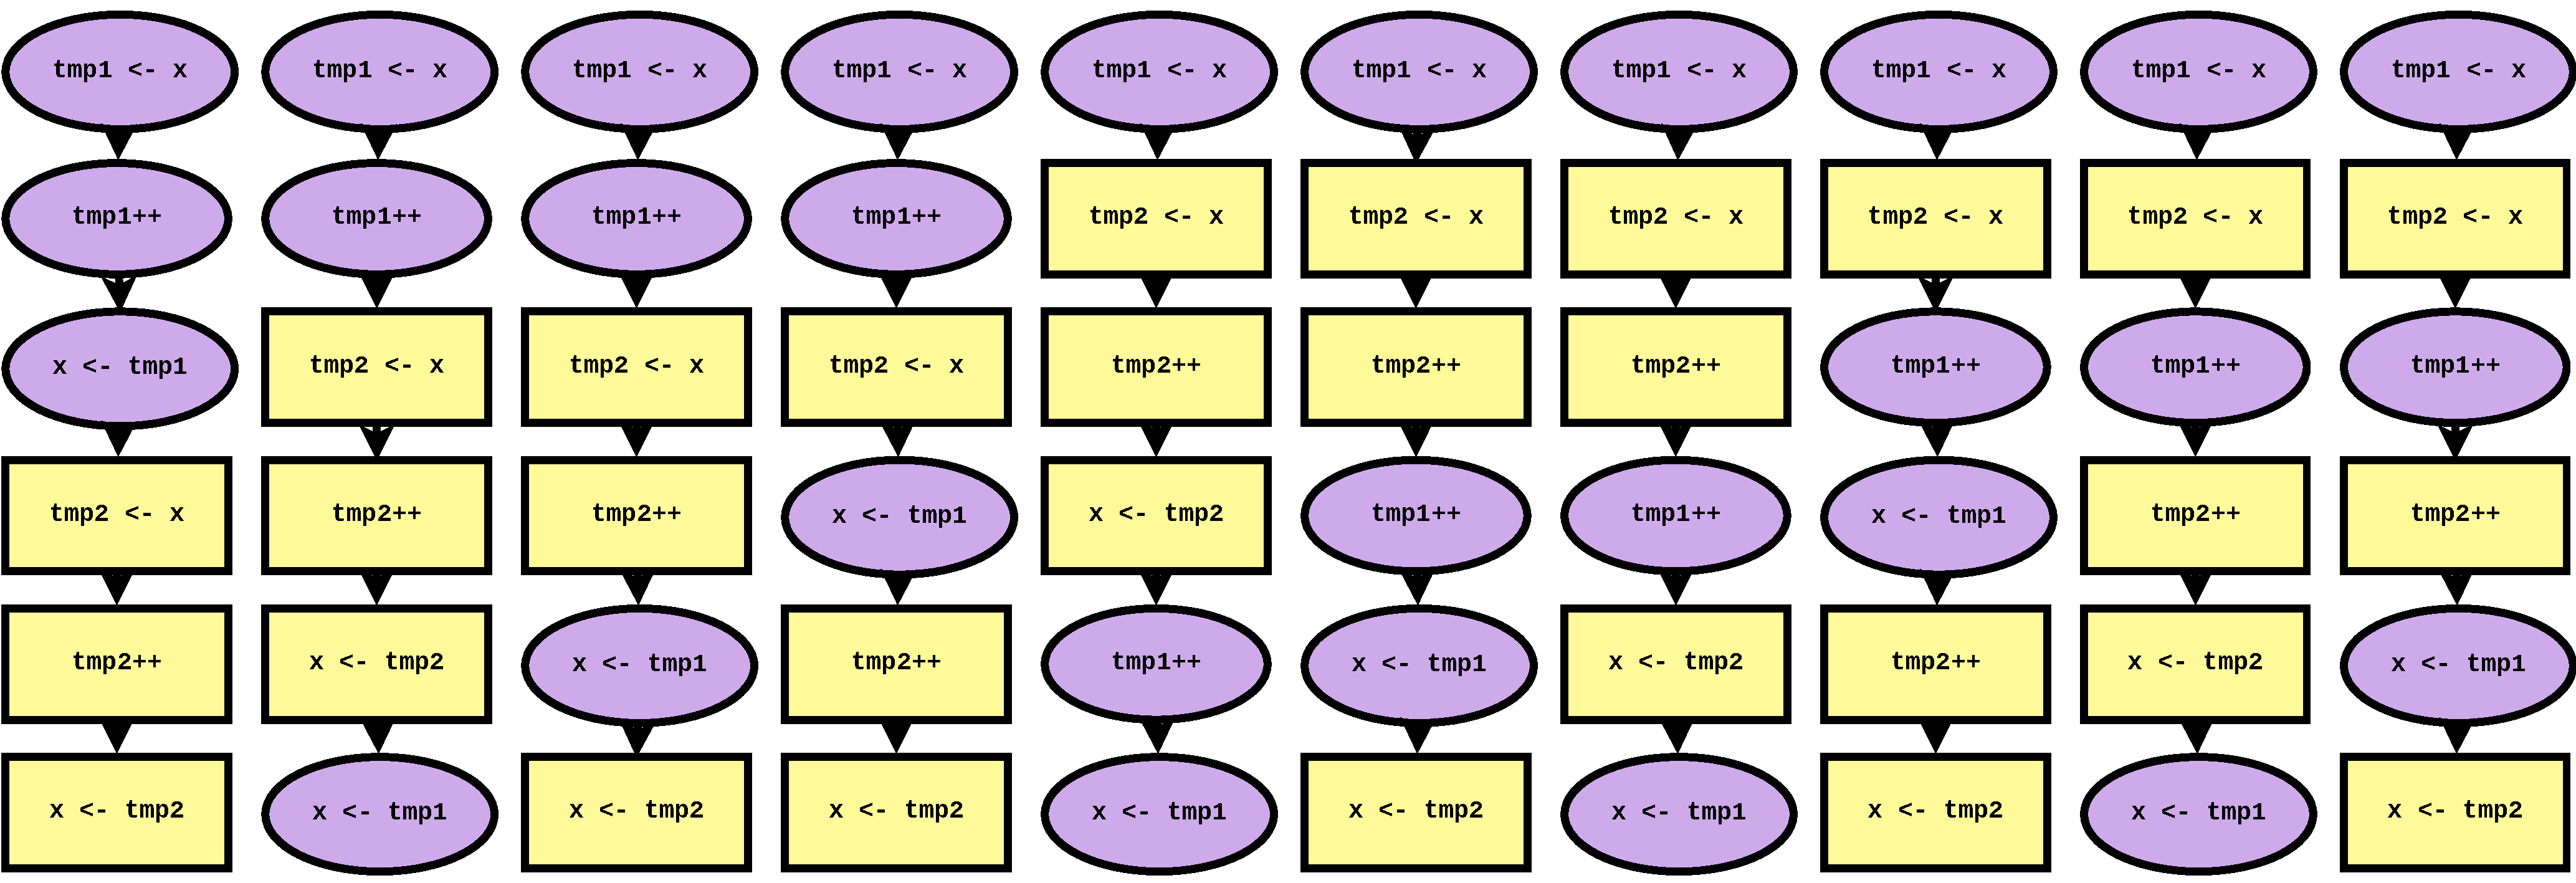
\includegraphics[width=\textwidth]{statespace-list.pdf}
		\\
		(a) Interleavings visualized individually, as a list.
		\\
		\\
		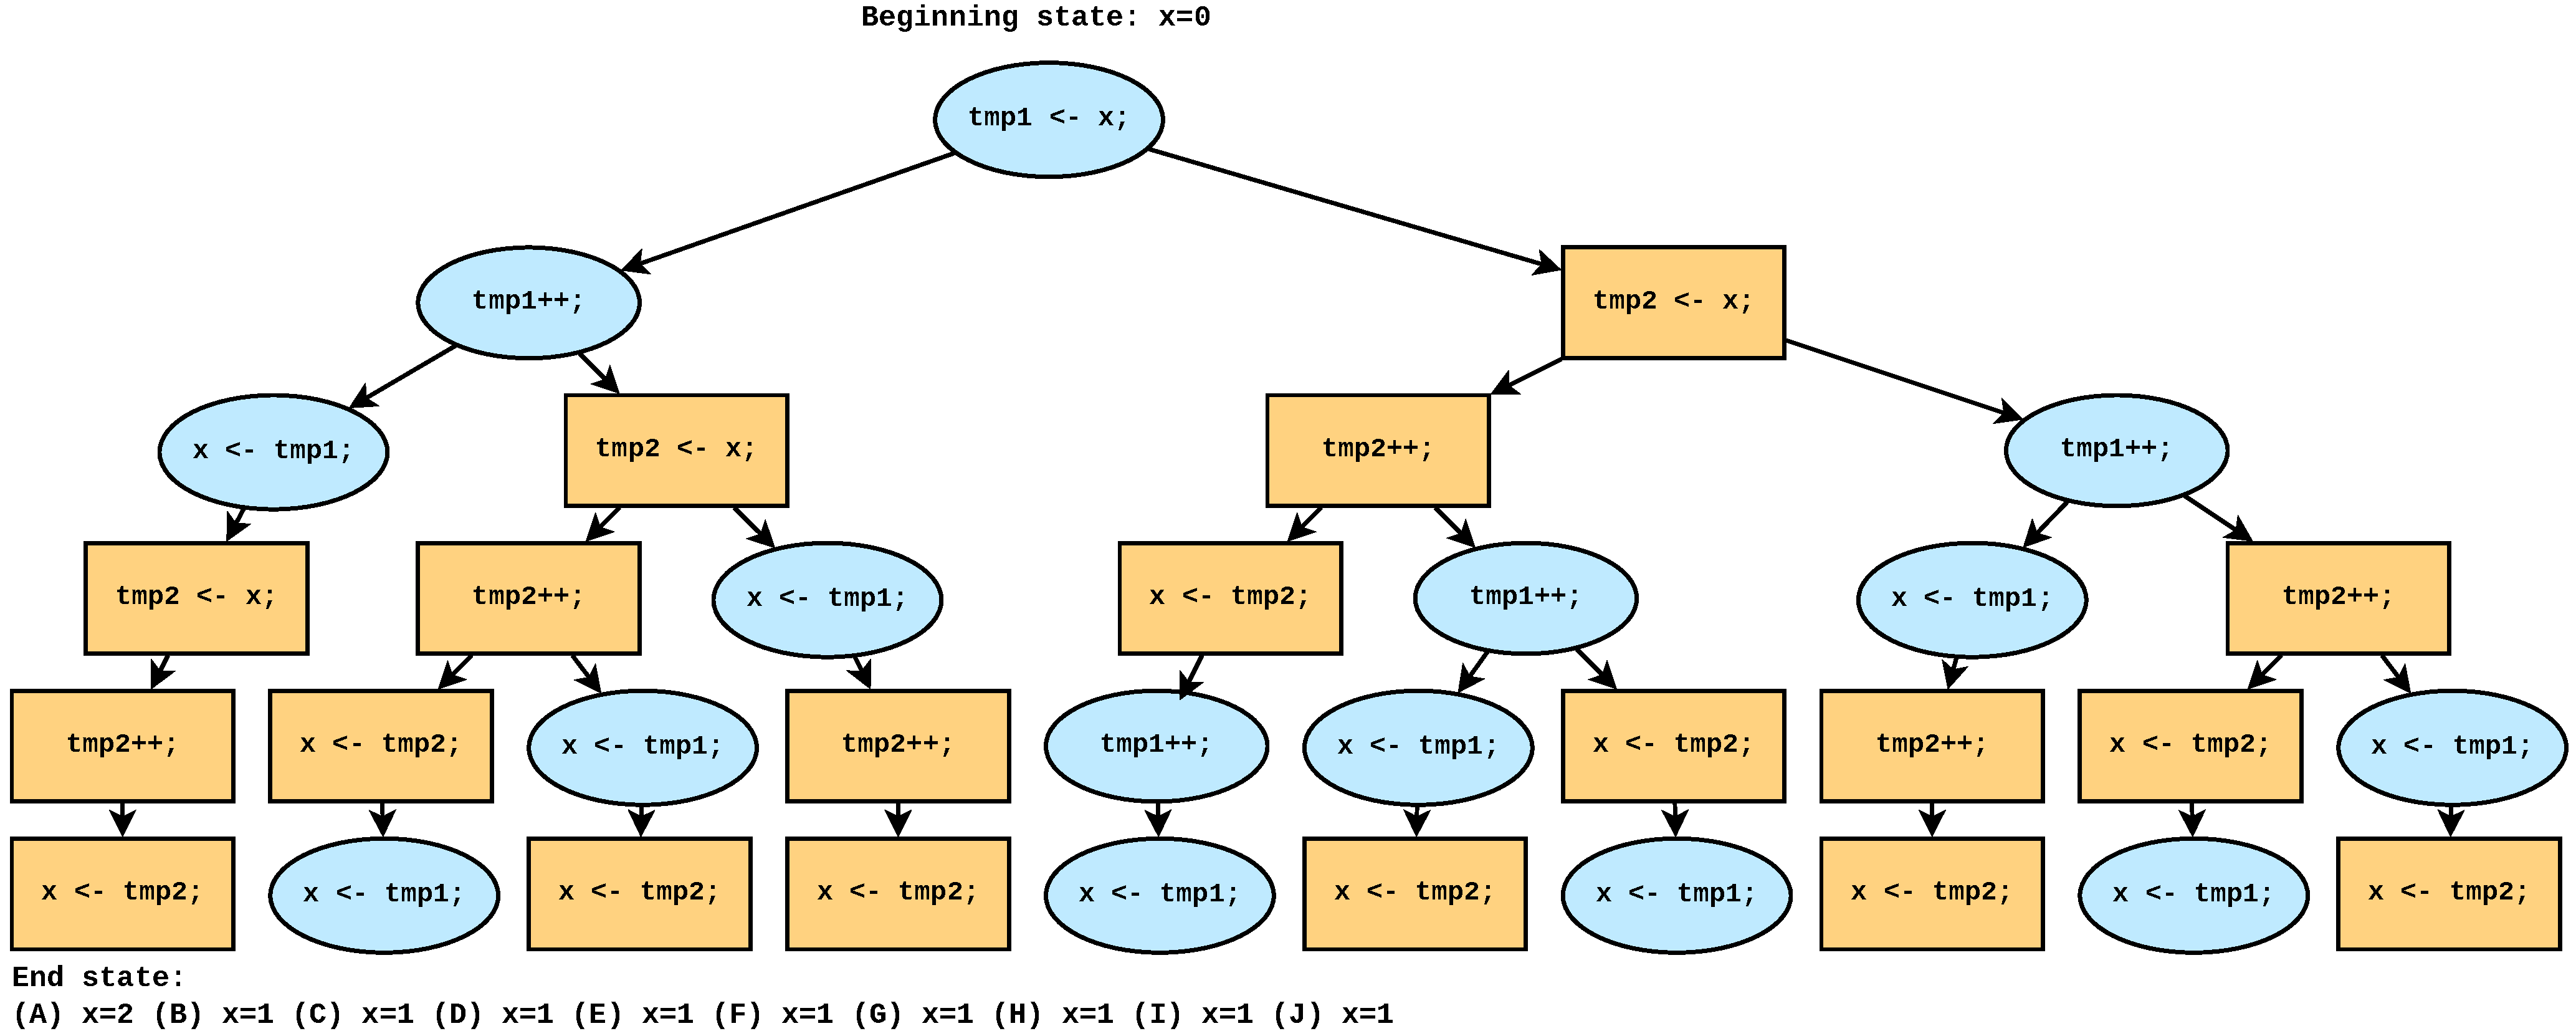
\includegraphics[width=\textwidth]{statespace-tree.pdf}
		\\
		(b) Interleavings (same order as in (a)), with common prefixes \\
		combined as ``preemption points'', forming a tree.
	\end{tabular}
	\caption{Visualization of interleaving state space for the program in Figure~\ref{fig:concurrency-bug}.
	Thread 1 is represented by purple ovals, thread 2 by yellow squares, and time flows from top to bottom.
	As the two threads execute the same code, without loss of generality thread 1 is fixed to run first --
	the full state space is twice the size, and the other half is symmetric to the one shown.}
	\label{fig:tree}
\end{figure}

Some model checkers explicitly store the set of visited program states as a means of identifying equivalent interleavings \cite{spin}.
This approach is called {\em stateful} model checking.
In this thesis, I focus on {\em stateless} model checking,
which instead analyzes the sequence of execution events to avoid a prohibitive memory footprint.
Henceforth I will abbreviate ``stateless model checking'' simply as ``model checking'' for brevity.

\subsubsection{Static versus dynamic analysis}

Model checking is a {\em dynamic} program analysis, meaning that it observes the operations and accesses performed by the program as its code is executed.
In contrast, {\em static} program analyses check certain properties at the source code level.
Static analyses are ideal for ensuring certain standards of code quality, which often correlates with correctness,
but cannot decide for certain whether a given program will fail during execution without actually running the code \cite{incompleteness}.
Static analyses face the challenge of {\em false alarms} (or {\em false positives}):
code patterns which look suspicious but are actually correct.
A debugging tool which reports too many false alarms will dissuade developers from using it \cite{racerx}.
Dynamic analysis, our approach, identifies program behaviours that are definitely wrong,
so each bug report is accompanied by concrete evidence of the violation.
Assertions, segfaults, use-after-free of heap memory, and deadlock are examples of such failures we check for,
although a checker may also include arbitrary program-specific predicates.

\subsubsection{Preemption points}

During execution, a model checker identifies a subset of the program's operations as ``interesting'', i.e.,
where interrupting the current thread to run a different one is likely to produce different behaviour.
These so-called {\em preemption points} may be identified by any combination of human intuition and machine analysis.
Typical preemption points include the boundaries of synchronization APIs (e.g., {\tt mutex\_lock}) or accesses to shared variables.
Considering that at each preemption point multiple threads exist as options to run next,
the set of possible ways to execute the program can be viewed as a tree.
Figure~\ref{fig:tree}(b) shows a visualization of the corresponding tree from our example program.

The number of preemption points in each execution defines the depth of this tree,
and the number of threads available to run defines the branching factor.
Hence, in a program with $n$ preemption points and $k$ threads available to run at each, the state space size is $O(n^k)$.
Nevertheless, to fully test all of a program's possible behaviours, we must check the executions corresponding to every branch of the tree.
Addressing the scaling problem in this exponential relation is the central research problem for all model checkers.

\subsection{On the size of state spaces}

At its essence, stateless model checking research is a perpetual struggle to become more and more efficient in order to test and verify bigger and bigger programs.
But whence this efficiency?
Techniques for coping with the exponential explosion fall into two categories:
(1) removing redundant interleavings from the state space when we can prove they are equivalent to some interleaving already tested,
or {\bf reduction techniques},
and
(2) prioritizing interleavings judged as more likely to contain bugs should bugs exist
in case we are unable to exhaustively test all interleavings after all,
or {\bf search heuristics}.

\subsubsection{Reduction techniques}

Dynamic Partial Order Reduction \cite{dpor} (henceforth, DPOR) is the most popular algorithm for mitigating the exponential explosion that arises as program size increases.

{\bf Abstractly speaking:}
Let {\em independent transitions} denote a pair of executions of two threads, each from one preemption point to the next,
in which there are no read/write or write/write access pairs to the same memory between threads.
DPOR reduces a state space, originally exponentially-sized in the number of thread transitions,
to an equivalent one
(i.e., testing which suffices to check all program behaviours that could arise in the original state space)
exponentially-sized in the number of {\em dependent} thread transitions.
%More intuitively, if two thread transitions between preemption points do not conflict on any shared resource access,
%reordering them produces an equivalent interleaving, i.e., the same program behaviour.
More technically, it identifies equivalent execution sequences according to Mazurkiewicz trace theory \cite{mazurkiewicz},
and tests at least one execution from each equivalence class.

{\bf Concretely speaking:}
Figure~\ref{fig:dpor} highlights part of an execution tree where the execution ordering of threads 1 and 2 are swapped,
and each interleaving has a respective ``subtree'' (i.e., possible interleavings given the fixed execution prefix leading up to it).
The specifics of execution before the thread 1/thread 2 sequence,
other possible threads to run instead of threads 1 or 2,
and what logic the program executes in those subtrees
are all presumably arbitrary.
In these two highlighted branches,
if the transitions of threads 1 and 2 are {\em independent},
%if the operations performed by threads 1 and 2 are independent
%(i.e., no write/read or write/write access pairs to the same memory),
DPOR deduces that the subsequent program states (indicated by the red arrow) are equivalent.
Thence, only one of the two interleavings and its respective subtree needs to be executed
in order to check all possible program states.
I explain how DPOR implements such a deduction in more detail in \sect{\ref{sec:landslide-dpor}}.

Over the years, researchers have developed many enhancements to DPOR, such as Optimal DPOR \cite{optimal-dpor}, parallelizable DPOR \cite{parallel-dpor}, SAT-directed model checking \cite{satcheck}, Maximal Causality Reduction \cite{mcr}, and DPOR for relaxed memory architectures \cite{tsopso}.

\begin{figure}[t]
	\begin{center}
	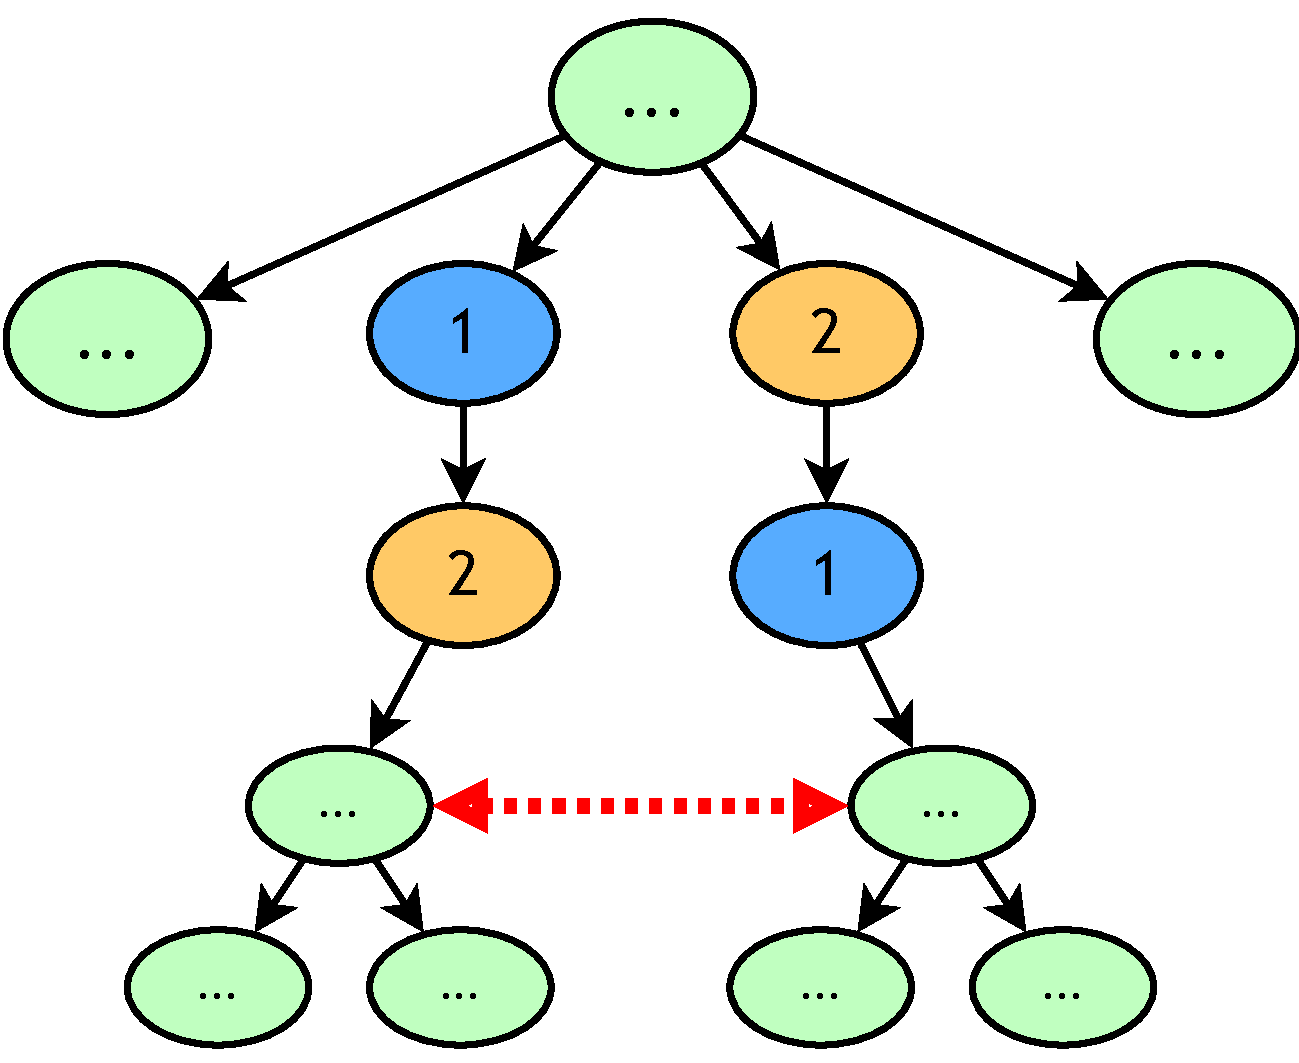
\includegraphics[width=0.4\textwidth]{dpor.pdf}
	\end{center}
	\caption{DPOR identifies independent transitions by different threads which can commute without affecting program behaviour. Here, if the transitions marked 1 and 2 have no shared memory conflicts, the states marked with the red arrow are guaranteed identical. Hence, only one of the subtrees need be explored.}
	\label{fig:dpor}
\end{figure}

\subsubsection{Search heuristics}

However, even though DPOR can prune an exponential number of redundant interleavings, the state space size is still exponential in the number of {\em dependent} (conflicting) interleavings.
Developers will always want to test larger and larger programs, so no matter the quality of our reduction algorithm,
we must accept that some tests will be too large to be fully tested in a reasonable time.
Hence, recent model checking research has turned to heuristic techniques for achieving further reduction,
optimizing the search to try to uncover bugs faster (should they exist)
at the expense of possibly missing other bugs,
or missing the chance to complete a full verification.

Iterative Context Bounding \cite{chess-icb} is a popular such technique which heuristically reorders the search to prioritize interleavings with fewer preemptions first.
This heuristic is based on the insight that most bugs require few preemptions to uncover, so interleavings with a number of preemptions that exceeds a certain bound will be de-prioritized, only tested until after all the fewer-preemption interleavings are completed.
Preemption sealing \cite{sealing} is another heuristic strategy which restricts the scope of the search by limiting the model checker to use only preemption points arising from certain functions in the source code.
This allows developers to vastly reduce state space size by identifying which program modules are already trusted,
although it requires some human intuition to correctly mark those boundaries.
Iterative Deepening, presented in Chapter~\ref{chap:quicksand}, is another such search heuristic.

%%%%%%%%%%%%%%%%%%%%%%%%%%%%%%%%%%%%%%%%%%%%%%%%%%%%%%%%%%%%%%%%%%%%%%%%%%%%%%%%

\section{Data Race Analysis}
\label{sec:background-datarace}

\begin{figure}[t]
        \small
	\begin{center}
\begin{tabular}{c}
\begin{tabular}{rll}
        & \multicolumn{2}{c}{\texttt{int x = 0; bool y = false; mutex\_t mx;}} \\
        \\
        & {\bf Thread 1} & {\bf Thread 2} \\
        1 & \texttt{\hilight{brickred}{x++;}~// A1} & \\
        2 & \texttt{mutex\_lock(\&mx);} & \\
        3 & \texttt{mutex\_unlock(\&mx);} & \\
        4 & & \texttt{mutex\_lock(\&mx);} \\
        5 & & \texttt{mutex\_unlock(\&mx);} \\
        6 & & \texttt{\hilight{brickred}{x++;}~// A2} \\
\end{tabular}
\\
\\
	{\normalsize (a) True potential data race.}
\\
\\
\begin{tabular}{rll}
        %& \multicolumn{2}{c}{\texttt{int x = 0; bool y = false; mutex\_t mx;}} \\
        & {\bf Thread 1} & {\bf Thread 2} \\
        1 & \texttt{\hilight{brickred}{x++;}~// B1} & \\
        2 & \texttt{mutex\_lock(\&mx);} & \\
        3 & \texttt{y = true;} & \\
        4 & \texttt{mutex\_unlock(\&mx);} & \\
        5 & & \texttt{mutex\_lock(\&mx);} \\
        6 & & \texttt{bool tmp = y;} \\
        7 & & \texttt{mutex\_unlock(\&mx);} \\
        8 & & \texttt{if (tmp) \hilight{brickred}{x++;}~// B2} \\
        %8 & & \texttt{if (tmp)} \\
        %9 & & \texttt{~~~~\hilight{brickred}{x++;}~// B2} \\
\end{tabular}
\\
\\
{\normalsize (b) No data race in any interleaving.}
\end{tabular}
	\end{center}
\caption{{Data-race analyses may be prone to either {\em false negatives} or {\em false positives}.
Applying Happens-Before to program (a) will miss the potential race possible between A1/A2 in an alternate interleaving,
while using Limited Happens-Before on (b) will produce a false alarm on B1/B2.}}
\label{fig:hb-example}
\end{figure}

\subsection{Definition}

Data race analysis \cite{eraser} identifies pairs of unsynchronized memory accesses between threads.
Two instructions are said to race if:
\begin{enumerate}
	\item they both access the same memory address,
	\item at least one is a write,
	\item the threads do not hold the same lock,
	\item and no synchronization enforces an order on the thread transitions (the {\em Happens-Before} relation, described below).
\end{enumerate}
%In Figure~\ref{fig:example}, lines 3 and 5 each race with 2 and 6, and line 6 races with 8.
In Figure~\ref{fig:hb-example}, the pairs of lines marked with comments (A1 and A2, B1 and B2) race.

A data race analysis may be either {\em static} (inspecting source code) \cite{racerx} or {\em dynamic} (tracking individual accesses arising at run-time) \cite{tsan}.
This paper focuses exclusively on dynamic analysis,
so although our example refers to numbered source lines for ease of explanation,
in practice we are actually classifying the individual memory access events corresponding to those lines during execution.
Actually, each {\tt x++} statement likely compiles to two separate load or store instructions, so each of those two instructions from each of the two marked source lines pairwise will race (except for the two loads, which are both reads).

\subsection{Happens-Before}
\label{sec:background-hb}

Condition 4 of the above definition expresses the notion that the access pair can be executed concurrently,
regardless of whether the hardware actually carries out the operations in the same physical instant.
Several approaches exist to formally representing this condition.

\begin{itemize}
	\item Most prior work focuses on {\em Happens-Before} \cite{lamport-clocks} as the order relation between accesses.
\cite{predictive-dr} and \cite{hybriddatarace} identify a problem with this approach:
it cannot identify access pairs separated by an unrelated lock operation which could race in an alternate interleaving,
as shown in the example program in Figure~\ref{fig:hb-example}(a).
We call such unreported access pairs {\em false negatives}.

\item
\cite{hybriddatarace} introduces the {\em Limited Happens-Before} relation,
which will report such potential races
by considering only blocking operations like {\tt cond\_wait} to enforce the order.
However, consider the similar program in Figure~\ref{fig:hb-example}(b),
in which the access pair ceases to exist in the alternate interleaving.
Limited Happens-Before will report all potential races, avoiding false negatives \cite{tsan},
but at the cost of necessarily reporting some such {\em false positives}.

\item
In recent work, the {\em Causally-Precedes} relation \cite{predictive-dr} %strikes a middle ground,
extends Happens-Before to additionally report a subset of potential races while soundly avoiding false positives.
It tracks conflicting accesses in intervening
critical sections to determine whether lock events are unrelated to a potential race.
Causally-Precedes will identify the potential race in Figure~\ref{fig:hb-example}(a), as the two critical sections do not conflict,
although it can still miss true potential races in other cases.
\end{itemize}

Landslide implements both Happens-Before (henceforth referred to as {\em Pure Happens-Before} for clarity) and Limited Happens-Before.
Chapter~\ref{chap:quicksand} includes a comparison of the two approaches for the purpose of finding new preemption points for model checking.
%, we use the Limited Happens-Before relation for our analysis.
%The justification for this is that, while stand-alone data-race analyses must avoid inundating the user with false alarms \cite{racerx},
%my work incorporates data-race analysis in an internal feedback loop, and reports only directly observed failures to the user.
%Hence, I accept some overhead from false positives for the sake of more thorough testing.

%%%%%%%%%%%%%%%%%%%%%%%%%%%%%%%%%%%%%%%%%%%%%%%%%%%%%%%%%%%%%%%%%%%%%%%%%%%%%%%%

\section{Education}
\label{sec:overview-edu}

In this thesis I will tackle Pebbles and Pintos, two different system architectures used in educational operating systems courses.
This section describes the projects which students implement and which Landslide tests.

\subsection{Pebbles}
\label{sec:pebbles}

The Pebbles kernel architecture
is used at Carnegie Mellon University (CMU) in 15-410, Operating System Design and Education \cite{kspec,thrlib}.
In the course of a semester, students work on five programming assignments;
the first two are individual, and the remaining three are the products of two-person teams.
I will focus on the third and fourth of these, the thread library and kernel,
called ``P2'' and ``P3'' respectively (the project numbers start at 0).
The other three (a stack-crawling backtrace utility, a bare-metal game with device drivers, and a small extension to the P3 kernel) are not of concern in this thesis.
The course's prerequisite is 15-213, Introduction to Computer Systems \cite{sigcse01:CSaPP}.
Both P2 and P3 are built using the {\em Pebbles} system call specification, outlined in Table~\ref{tab:syscalls}

\begin{table}
        \center
        \begin{tabular}{|l|p{0.75\textwidth}|}
                \hline
                \bf System call name & \bf Summary \\
                \hline
                \multicolumn{2}{c}{\em Lifecycle management} \\
                \hline
                \texttt{fork} & Duplicates the invoking task, including all memory regions. \\
                \texttt{thread\_fork} & Creates a new thread in the current task.\\
                \texttt{exec} & Replaces the program currently running in the invoking task with a new one specified. \\
                \texttt{set\_status} & Records the exit status of the current task. \\
                \texttt{vanish} & Terminates execution of the calling thread. \\
                \texttt{wait} & Blocks execution until another task terminates, and collects its exit status.\\
                \texttt{task\_vanish}* & Causes all threads of a task to \texttt{vanish}. \\
                \hline
                \multicolumn{2}{c}{\em Thread management} \\
                \hline
                \texttt{gettid} & Returns the ID of the invoking thread. \\
                \texttt{yield} & Defers execution to a specified thread. \\
                \texttt{deschedule} & Blocks execution of the invoking thread. \\
                \texttt{make\_runnable} & Wakes up another \texttt{deschedule}d thread. \\
                \texttt{get\_ticks} & Gets the number of timer ticks since bootup. \\
                \texttt{sleep} & Blocks a thread for a given number of ticks. \\
                \texttt{swexn} & Registers a user-space function as a software exception handler.\\
                \hline
                \multicolumn{2}{c}{\em Memory management} \\
                \hline
                \texttt{new\_pages} & Allocates a specified region of memory. \\
                \texttt{remove\_pages} & Deallocates same. \\
                \hline
                \multicolumn{2}{c}{\em Console I/O} \\
                \hline
                \texttt{getchar}* & Reads one character from keyboard input. \\
                \texttt{readline} & Reads the next line from keyboard input. \\
                \texttt{print} & Prints a given memory buffer to the console. \\
                \texttt{set\_term\_color} & Sets the color for future console output. \\
                \texttt{set\_cursor\_pos} & Sets the console cursor location. \\
                \texttt{get\_cursor\_pos} & Retrieves the console cursor location. \\
                \hline
                \multicolumn{2}{c}{\em Miscellaneous} \\
                \hline
                \texttt{ls} & Loads a given buffer with the names of files stored in the RAM disk ``file system.'' \\
                \texttt{halt} & Ceases execution of the operating system. \\
                \texttt{misbehave}* & Selects among several thread-scheduling policies. \\
                \hline
        \end{tabular}
        \caption{The Pebbles specifcation defines 25 system calls. Students are not required to implement ones marked with an asterisk (*), though the reference kernel provides them. }
        \label{tab:syscalls}
\end{table}

\subsubsection{P2}
The thread library project \cite{thrlib} has two main components: implementing concurrency primitives, and implementing thread lifecycle and management routines.
The required concurrency primitives are as follows:
\begin{itemize}
	\item Mutexes, with the interface {\tt mutex\_lock(mp)} and {\tt mutex\_unlock(mp)}, whose functionality is described earlier this chapter. Students may use any x86 atomic instruction(s) they desire, such as {\tt xchg}, {\tt xadd}, or {\tt cmpxchg}, and/or the {\tt deschedule}/ {\tt make\_runnable} system calls offered by the reference kernel.
	\item Condition variables, with the interface {\tt cond\_wait(cvp, mp)}, {\tt cond\_signal} {\tt (cvp)}, and {\tt cond\_broadcast(cvp)}. {\tt cond\_wait} blocks the invoking thread, ``simultaneously'' releasing a mutex which protects some associated state (atomically, with respect to other calls to signal or broadcast under that mutex).
		{\tt cond\_signal} and {\tt cond\_broadcast} wake one or all waiting threads.
		Students must use the {\tt deschedule} and {\tt make\_runnable} system calls to implement blocking (busy-waiting is forbidden), and typically include an internal mutex to protect the condition variable's state as well.
		The primary challenge of this exercise is ensuring the aforementioned atomicity between {\tt cond\_wait}'s unlock and deschedule, with respect to the rest of the interface.
	\item Semaphores, with the interface {\tt sem\_wait(sp)} and {\tt sem\_signal(sp)} (sometimes called {\em proberen} and {\em verhogen} in other literature). The semaphore can be initialized to any integer value; if initialized to 1, it behaves like a mutex.
		Students typically implement semaphores using mutexes and condition variables, not using atomic instructions or system calls directly.
	\item Reader-writer locks (rwlocks), with the interface {\tt rwlock\_lock(rwp, mode)} and {\tt rwlock\_unlock(rwp)}. {\tt mode} may be either {\tt RWLOCK\_READ} or {\tt RWLOCK\_\allowbreak{}WRITE}.
		Behaves as mutexes, but multiple readers may access the critical section simultaneously.
		Students typically implement rwlocks using mutexes and condition variables, not using atomic instructions or system calls directly.
\end{itemize}
The interface to each also includes an associated {\tt \_init()} and {\tt \_destory()} function.

The thread lifecycle/management routines are as follows:
\begin{itemize}
	\item {\tt thr\_init(stack\_size)} initializes the thread library, setting a default stack size to be allocated to new threads.
	\item {\tt thr\_create(child\_func, child\_arg)} spawns a new thread to run the specified function with the specified argument. There is a semantic gap between this function and the {\tt thread\_fork} system call (which takes no parameters, makes no changes to the user's address space, and cannot meaningfully be invoked from C code) which students must bridge.
		Returns an integer thread ID of the newly created thread.
	\item {\tt thr\_exit(status)} aborts execution of the calling thread, recording an exit status value.
		The main challenge of this function is to allow another thread to free the memory used for the exiting thread's stack,
		without risking any corruption as long as the exiting thread continues to run.
	\item {\tt thr\_join(tid, statusp)} blocks the calling thread until the thread with the specified thread ID exits, then returns, collecting its exit status.
\end{itemize}
Other than {\tt thr\_init} (which is necessarily single-threaded), several concurrency errors between any two (or all three) of these functions are very common in student submissions.

Finally, students also implement automatic stack growth using the {\tt swexn} system call, which is not relevant to this thesis.

\subsubsection{P3}
In P3, students implement a kernel which provides the same system calls shown in Table~\ref{tab:syscalls}, previously provided by the reference kernel.
Pebbles adopts the Mach \cite{DBLP:conf/usenix/AccettaBBGRTY86} distinction between {\em tasks}, which are resource containers, and {\em threads}, each of which executes within a single task.
This requires less implementation complexity than the more featureful Plan 9's {\tt rfork} \cite{Pike90plan9} or Linux's {\tt clone} models.

Although the internal interfaces are not mandated like they were in P2, all Pebbles kernels must necessarily contain the same abstract components. These include:
\begin{itemize}
	\item A round-robin scheduler, including context switching, timer handling, and runqueue management;
	\item Some approach to locking, often analogous to P2's concurrency primitives (henceforth referred to as ``kernel mutexes''), 
	 ll       and some approach to blocking threads indefinitely;
	\item A virtual memory implementation, including a program loader;
	\item Lifecycle management code for creation and destruction of kernel threads and processes;
	\item Other miscellany such as a suite of fault handlers to ensure no user program can cause the kernel itself to crash.
\end{itemize}
Because any combination of system calls or fault handlers can be invoked by user programs simultaneously,
concurrency bugs can arise from the interaction of any subset of kernel components with each other.
The most common bugs studence face arise from the interaction of some component with itself (e.g., concurrent invocations of {\tt new\_pages}/{\tt remove\_pages} in the same process),
or from the interaction between an exiting thread and some other thread trying to communicate with it ({\tt vanish} versus, well, anything else, really).
The most difficult concurrency problem in P3 is that of coordinating a parent and a child task that simultaneously exit:
when a task completes, live children and exited zombies must be handed off to the task's parent or to the {\tt init} process,
when the task's parent may itself be exiting;
meanwhile, threads in tasks that receive new children may need to be awakened from {\tt wait}.
Careless solutions to this problem are prone to data races or deadlocks.

% TODO: Talk about the hurdle (both for p2 and p3).

\subsubsection{Secrecy}
\label{sec:410-secrecy}

The 15-410 course staff is notoriously secretive about the nature of many concurrency bugs
students commonly encounter during P2 and P3.
This is driven by a desire to cause students to find, diagnose, and fix these bugs on their own during the projects,
rather than to be surprised by them afterwards during grading
\cite{de0u-2018}.
%
One such example is the {\tt paraguay} unit test distributed with P2 (\sect{\ref{sec:education-pebbles-tests}}),
which targets a subtle condition-variable bug.
The test uses the {\tt misbehave} system call to target a particular thread interleaving likely to expose the bug
which is otherwise very unlikely to arise in normal execution.
The reference kernel specification \cite{kspec} does not define the {\tt misbehave} modes' behaviours,
as doing so would deprive students of the learning experience of discovering the interleaving in question on their own.
%
In this thesis I will occasionally use intentionally vague phrasing to preserve the mystery of these bugs.

\subsubsection{Use at other universities}
\label{sec:overview-psu}

\newcommand\psuos{CMPSC 473\xspace}

In the Spring 2018 semester,
the Operating Systems class at Penn State University (henceforth \psuos and PSU, respectively)
offered the P2 thread library project as part of its curriculum.
Students in this class implement P2
on a 6 week project timeline (compared to 2 weeks at CMU),
work alone rather than in pairs,
skip the {\tt swexn} automatic stack growth portion,
and rather than running their code with a reference Pebbles kernel binary in a simulator,
use the Pebwine emulation layer \cite{pebwine}
to run Pebbles-compatible program binaries in the Linux userspace.
Otherwise, the project is identical to CMU 15-410's P2.

\subsection{Pintos}
\label{sec:overview-pintos}

\newcommand\uchos{CMSC 23000\xspace}

The Pintos kernel architecture \cite{pintos} is used at several universities, including Berkeley, Stanford, and the University of Chicago.
The Pintos basecode implements a rudimentary kernel, consisting of a context switcher, round-robin scheduler, locking primitives, and program loader.
upon which students add more features in several projects.
Most relevant to this thesis, the basecode provides the following functions/libraries, among others:
\begin{itemize}
	\item Semaphores (the basic concurrency primitive, implemented using direct scheduler calls): {\tt sema\_up}, {\tt sema\_down}, {\tt sema\_try\_down};
	\item Locks (which wrap a semaphore initialized to 1), {\tt lock\_acquire}, {\tt lock\_\allowbreak{}release}, {\tt lock\_try\_acquire};
	\item Condition variables (also implemented using scheduler calls): {\tt cond\_wait}, {\tt cond\_\allowbreak{}signal}, {\tt cond\_broadcast}, with the same semantics as Pebbles P2 condvars;
	\item Basic round-robin scheduling facilities: {\tt thread\_block} (a kernel-level analogue to Pebbles's {\tt deschedule}), {\tt thread\_yield}
	\item Kernel thread lifecycle management, {\tt thread\_create} and {\tt thread\_exit}, including stack space memory management;
	\item Interrupt and fault handlers;
	\item A page allocator, {\tt palloc\_get\_page}, {\tt palloc\_get\_multiple}, {\tt palloc\_free\_page}, and {\tt palloc\_free\_multiple}
\end{itemize}
Both Pebbles and Pintos basecodes offer a standard C library including {\tt malloc}, string-formatting, printing, etc.

Although there is some variety in supplemental assignments, all Pintos courses include three core projects building on the Pintos basecode:
\begin{itemize}
	\item {\em Threads}: Students must implement an ``alarm clock'' (analogous to Pebbles's {\tt sleep} system call),
		a priority scheduling algorithm, and a multi-level feedback queue scheduler.
		% TODO: Later. Talk about how concurrency testing can only test certain parts of this crap.
	\item {\em Userprog}: Provided with rudimentary virtual memory and ELF loader implementations, students must implement argument passing and several system calls associated with userspace programs, including {\tt exec}, {\tt exit}, {\tt wait}, and file descriptor management.
	\item {\em Filesys}: Provided with a simple ``flat'' filesystem implementation, students must extend it with a buffer cache, extensible files, and subdirectories.
\end{itemize}

Some schools further offer a virtual memory project, extending the provided VM with a frame table and supplemental page table and fault handler \cite{standford-cs140,uchicago-cs230}, or supplemental HTTP server and {\tt malloc} assignments \cite{berkeley-cs162}.
Being largely architectural/algorithmic projects rather than concurrency-oriented ones, I am not concerned with these assignments in this thesis.
The main concurrency challenges in Pintos projects arise from the {\em threads} and {\em userprog} assignments:
implementing a correct {\tt alarm} routine,
ensuring the priority scheduler remains safe in the presence of concurrent threads of the same priority,
and designing correct interactions between the {\tt wait} and {\tt exit} system calls.

\section{Glossary}
\label{sec:glossary}

This section provides a convenient reference of terminology used throughout the thesis.

% TODO

% concurrency bug
% race condition: "a confusing term which in some circles means concurrency bug and others data race, which we will avoid"
% data race
% atomicity violation (what even is this.)
% thread
% transition
% conflict
% independent: "see conflict"
% state space
% interleaving
% DPOR
% estimation (WBE, RE)
% landslide
% quicksand
% iterative deepening
% MC, stateless MC
% TA: teaching assistant
% P2 (note abotu psu - dosent call it p2, but we call it that for both schools here
% happens before, all 3 versions - DPOR, LHB, and PHB
% userspace, kernelspace

% TODO: scan for abbrs like PP, MC, SSS-MC - well mc is ok but rephrase if necessary anyway
\chapter{Quicksand}
\label{chap:quicksand}

% https://tex.stackexchange.com/questions/186746/define-shearbox-with-rotatebox-and-scalebox
\newcommand\xshearbox[2]{%
  \FPeval{\sheark}{(root(2,(#1)*(#1)+4)+#1)/2}\FPeval{\shearl}{1/\sheark}%
  \FPeval{\sheara}{arctan(-\sheark)*180/pi}\FPeval{\shearb}{90+\sheara}%
  \rotatebox{\shearb}{\scalebox{\sheark}[\shearl]{{\rotatebox{\sheara}{\smash{#2}}}}}%
}

\inspirationalquote{
% original - on second thought, i'm not actually gonna put this in
% the nuance in japanese is more desperate, more disorganized, and less generally heroic-seeming
% i think the english translation actually works better for an inspirational quote
%{\footnotesize 嫌な事も悲しい事もあったけど、守りたい物だってたくさんこの世界にはあったから。} \\
There are awful, sad things in this world.
But there are a lot of things worth protecting, too.
}
%{Kaname Madoka, Mahou Shoujo Madoka{\raisebox{0.1em}{$\scriptstyle \bigstar$}}Magica}
{Kaname Madoka, Puella Magi Madoka{\raisebox{0.1em}{\scalebox{0.65}{\xshearbox{0.25}{$\bigstar$}}}}Magica}
%\inspirationalquote{Always, somewhere, someone is fighting for you.
%As long as you remember her, you are not alone.}
%{Mahou Shoujo Madoka{\raisebox{0.1em}{$\scriptstyle \bigstar$}}Magica}

\vspace{2em}
\qrevision{There is a fundamental disconnect between existing stateless model checkers
and human users
when it comes to testing concurrent code meaningfully within a fixed CPU budget.
Existing tools
%are configured to
test systems according to a fixed preemption strategy,
leading to runtime dependent entirely on the complexity of the test program,
which may range from minutes to tens of thousands of years.
Meanwhile, users approach testing with a finite amount of patience,
%usually in the rough order of magnitude of a day:
usually not varying from one test cycle to another as their code changes and evolves:
students frantically testing last-minute changes facing a project deadline
will likely wait no longer than an hour for test results,
while a company preparing its product for production deployment % its, not their. companies arent people :triumph:
may spend upwards of weeks on rigorous stability testing.
Regardless of the use case,
a stateless model checker committing in advance to test whichever single state space arises from its fixed strategy
is certain to either under- or over-shoot its user's needs.
A model checker which preempts the system too often will fail to complete the test in time,
and one which preempts infrequently enough to complete with time to spare will leave the user wondering if it overlooked any bugs.

This chapter presents Quicksand,
an execution framework for model checking to manage this trade-off at run-time.
Given a fixed CPU budget,
representing the user's patience for testing,
Quicksand dynamically alters its preemption strategy based on data race analysis
(\cite{tsan,fasttrack}, \cref{sec:landslide-datarace})
and optimizes the size of state spaces on the fly,
guided by state space estimation
(\cite{estimation}, \cref{sec:landslide-estimate}),
to best match that budget.
I will discuss the trade-off inherent in number of preemption points used
(\cref{sec:quicksand-motivation}),
introduce {\em Iterative Deepening},
the algorithm that Quicksand uses to automatically navigate that trade-off
(\cref{sec:quicksand-id}),
prove its soundness relative to the more expensive full verification approach
(\cref{sec:quicksand-soundness}),
and present a large evaluation of Quicksand against several
state-of-the-art approaches % implemented under Landslide
in which Quicksand performs best on both bug-finding and verification
(\cref{sec:quicksand-eval}).
% justifying the claim that model checkers should navigate said tradeoff at runtime
}

The contributions of this chapter were published as
{\em Stateless Model Checking with Data-Race Preemption Points}
in OOPSLA 2016 \cite{quicksand}.

%%%%%%%%%%%%%%%%%%%%%%%%%%%%%%%%%%%%%%%%%%%%%%%%%%%%%%%%%%%%%%%%%%%%%%%%%%%%%%%%
%%%%%%%%%%%%%%%%%%%%%%%%%%%%%%%%%%%%%%%%%%%%%%%%%%%%%%%%%%%%%%%%%%%%%%%%%%%%%%%%
%%%%%%%%%%%%%%%%%%%%%%%%%%%%%%%%%%%%%%%%%%%%%%%%%%%%%%%%%%%%%%%%%%%%%%%%%%%%%%%%

\section{Motivation}
\label{sec:quicksand-motivation}

\qrevision{When configuring a model checker's preemption strategy,
or indeed,
choosing a model checker to begin with,
the resulting state space is {\em parameterized} by the set of preemption points.
%
In the first example of \Cref{fig:tree}
I constructed the state space by expanding both threads' {\tt x++} operations into three pseudo-assembly instructions,
then designating every instruction as a possible preemption point,
yielding ${3+3 \choose 3} = 20$ total interleavings.
Later, \cref{sec:landslide-dpor} showed that DPOR prunes 16 of those as equivalent,
although the reduced state space size is still combinatorial
in the number of {\em conflicting} events, rather than the total number.
For larger tests, %with hundreds or thousands of conflicting events in any given execution,
committing in advance to test all possible interleavings quickly becomes impractical.
Accordingly, many existing model checkers opt for preempting on only a subset of execution events,
such as synchronization API boundaries.

\subsection{Preemption points}
\label{sec:quicksand-pps}

Consider the new example program in \Cref{fig:pps-example}(a),
in which one thread protects its accesses to {\tt count} with a mutex,
while the other protects its accesses with atomic increment instructions.
Assuming {\tt count} is only ever incremented, never decremented,
the assertion in Thread 2 expects both of its preceding increments to be visible,
no matter how many other threads come incrementing % incrementしてくる
{\tt count} simultaneously.
However, this assumes any other accesses to {\tt count} use the same protection mechanism,
i.e., {\tt atomic\_xadd()},
but since Thread 1 uses a mutex (which Thread 2 never touches),
the threads can interleave to cause the assert to fail,
as shown in \Cref{fig:pps-example}(b).
%
\Cref{fig:pps-statespace} shows the resulting state space
supposing the model checker preempts only on synchronization APIs.%
\footnote{Most modern C/C++ programs invoke atomic memory instructions by using compiler intrinsics,
which could themselves be instrumented as a known synchronization API.
However, not all programs are guaranteed to use well-understood interfaces;
in fact, in the 15-410 class projects to be tested in the upcoming evaluation (\cref{sec:quicksand-eval-suite}),
students are encouraged to roll their own atomics to get more experience writing x86 assembly.
For the sake of this example, I leave {\tt atomic\_xadd()} uninstrumented.}
However, \Cref{fig:pps-example}(b)'s interleaving involves
preempting Thread 1 between its load and store of {\tt count},
which is not a known synchronization call, but rather a data race.
Hence, none of the interleavings in \Cref{fig:pps-statespace}'s state space
will expose the failure;
a {\em data-race preemption point} is required to find this bug.

\begin{figure}[t]
	\begin{center}
		\begin{tabular}{p{0.8\textwidth}}
			\begin{center}
			\begin{tabular}{ll}
				\multicolumn{2}{c}{Initially {\tt int count = \const{0}; mutex\_t m;}} \\
				\\
				{\bf Thread 1} & {\bf Thread 2} \\
				\hline
				\texttt{\hilight{darkorange}{mutex\_lock}(\&m);} & \texttt{atomic\_xadd(\&count, \const{1});} \\
				\texttt{count++;}                                & \texttt{\hilight{olivegreen}{yield}();} \\
				\texttt{\hilight{darkblue}{mutex\_unlock}(\&m);} & \texttt{atomic\_xadd(\&count, \const{1});} \\
				\texttt{assert(count >= \const{1});}      & \texttt{assert(count >= \const{2});} \\
			\end{tabular}
			\end{center}
			\\
			(a) Example program with synchronization API calls highlighted.
			\\
			\\
			\begin{center}
			\begin{tabular}{llc}
				{\bf Thread 1} & {\bf Thread 2} & {\bf Value of {\tt count}} \\
				\hline
				\texttt{\hilight{darkorange}{mutex\_lock}(\&m);} & & 0 \\
				\texttt{int tmp = count;} & & 0 \\
							& \texttt{atomic\_xadd(\&count, \const{1});} & 1 \\
							& \texttt{\hilight{olivegreen}{yield}();} & 1 \\
							& \texttt{atomic\_xadd(\&count, \const{1});} & 2 \\
				\texttt{count = tmp + 1;} & & 1 \\
							& \texttt{\hilight{assertfail}{assert(count >= 2);}} & 1 \\
				\texttt{\hilight{darkblue}{mutex\_unlock}(\&m);} & & 1 \\
				\texttt{assert(count >= \const{1});} & & 1 \\
			\end{tabular}
			\end{center}
			\\
			(b) Interleaving of (a) in which Thread 2's assertion fails,
			as the single increment of Thread 1 overwrites both those of Thread 2.
		\end{tabular}
	\end{center}
	\caption[Example bug requiring data-race preemption points to expose.]
	{Example bug requiring data-race preemption points to expose.
	Because the two threads use different modes of synchronization to protect their respective accesses to {\tt count},
	preempting on synchronization calls alone is insufficient to expose the bug.
	Rather, Thread 1 must be preempted between its non-atomic load and store of {\tt count}.
	}
	\label{fig:pps-example}
\end{figure}

\begin{figure}[ht!] % TODO: check placement
	\begin{center}
		% FIXME: fix it to be a real tree
		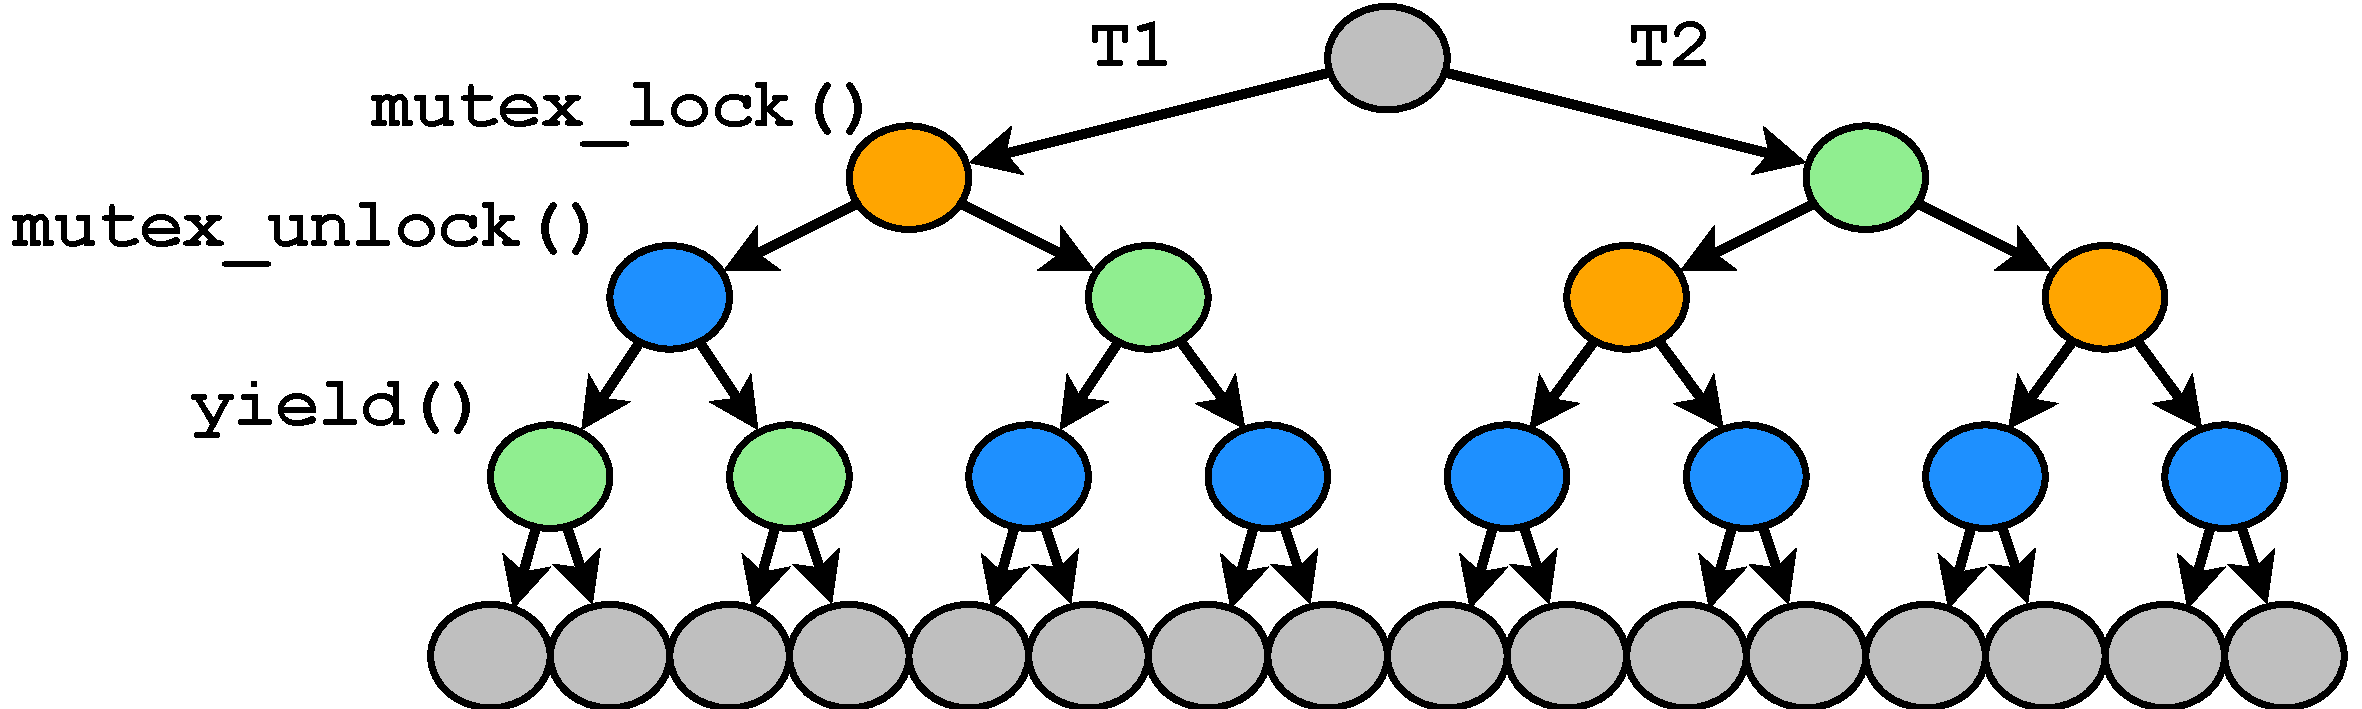
\includegraphics[width=0.9\textwidth]{../oopsla/tree-maximal-only.pdf}
	\end{center}
	\caption[State space of \Cref{fig:pps-example} with synchronization preemption points only.]
	{State space of \Cref{fig:pps-example} with synchronization preemption points only.
	Note that none of these interleavings preempt Thread 1 at the necessary place
	to trigger Thread 2's assertion failure.}
	\label{fig:pps-statespace}
\end{figure}
}

\qrevisionminor{How should a model checker know to instrument this particular data race for preemption
in order to find the assertion failure lurking underneath?}
Committing in advance to
preempt on every instruction is certain to include this data race,
but invites massive state space explosion.
Even as DPOR helps to skip equivalent interleavings of non-conflicting transitions,
DPOR itself is $O(n^2)$ in the number of preemption points in a single execution,
which is not compatible with such an approach.
Accordingly, stateless model checkers must find more efficient ways to be able to uncover bugs such as these.
%
In related work,
Portend~\cite{portend} proposed to combine data race analysis with preemption-driven artificial scheduling,
although it obtains its data race candidates from a stand-alone, single-pass analysis.
In order to
%make sure we
identify every
%one of a program's
data race that could possibly arise under the given test case,
a model checker must check many different interleavings to begin with,
perform the Portend approach for every data race it finds,
which may in turn uncover more data races
(hidden in flow control paths reachable only through interleavings of the first race, perhaps),
and then continue model checking those multiple races together
in a
%sort of
bidirectional feedback loop between the two algorithms.
Upcoming,
\cref{sec:quicksand-id} will show how I achieve this in Quicksand, and
\cref{sec:quicksand-soundness} will justify the technique's formal verification power.
In the evaluation, %(\cref{sec:quicksand-eval}),
\qrevisionminor{\cref{sec:quicksand-eval-bugs} and \cref{sec:quicksand-eval-verif}
will show that Quicksand strikes a healthy balance between fast bug-finding and full verification,
and
\cref{sec:quicksand-eval-nondets}
%in particular
will justify the need
for such a feedback loop %between model checking and data race analysis.
by showing that many
data races require model checking to reliably detect.
%bugs require nondeterministic data races to expose.
}

\subsection{Terminology}
\label{sec:quicksand-terminology}

\qrevision{For the rest of this chapter, I will use the following terminology as shorthand for the concepts explained above.

\begin{itemize}
	\item {\bf Single-state-space model checking} refers to the state-of-the-art model checking strategy,
		i.e., approaching each test with preemption points fixed in advance.
	\item {\bf Maximal state space} refers to the set of thread interleavings possible
		by preempting on all currently-known preemption points,
		whether synchronization or data-race,
		i.e., the singular state space tested by {\em single-state-space model checking}.
	\item {\bf Minimal state space} indicates the opposite:
		those thread interleavings requiring no more than Landslide's mandatory preemptions on voluntary context switches.
	\item {\bf Data-race bug}
		will refer to a concrete failure, such as \Cref{fig:pps-example}'s assertion failure above, whereas
	\item {\bf Data race} refers to the racing access pair itself (\cref{sec:landslide-datarace}).
	\item {\bf Data race candidate} shall refer specifically to
		potentially-racing accesses identified by Limited Happens-Before, %(\cref{sec:landslide-lhb}), % sub sub sec
		when disambiguation with {\em data races} is necessary.
	\item {\bf Benign data races} are those that, when reordered in an alternate interleaving,
		do not lead to a {\em data-race bug}, while
	\item {\bf False positives} are {\em data race candidates} that,
		upon trying to reorder them,
		turn out not to exist in the alternate interleaving at all,
		such as in \Cref{fig:hb-example}(b).
	\item {\bf Nondeterministic data race}
		will refer to data races that cannot be exposed on the first thread interleaving,
		but require model checking to expose to begin with.
\end{itemize}
}

%%%%%%%%%%%%%%%%%%%%%%%%%%%%%%%%%%%%%%%%%%%%%%%%%%%%%%%%%%%%%%%%%%%%%%%%%%%%%%%%
%%%%%%%%%%%%%%%%%%%%%%%%%%%%%%%%%%%%%%%%%%%%%%%%%%%%%%%%%%%%%%%%%%%%%%%%%%%%%%%%
%%%%%%%%%%%%%%%%%%%%%%%%%%%%%%%%%%%%%%%%%%%%%%%%%%%%%%%%%%%%%%%%%%%%%%%%%%%%%%%%

\section{Iterative Deepening}
\label{sec:quicksand-id}

To address the problem of choosing meaningful preemption points,
I have developed an algorithm called {\em Iterative Deepening},
implemented in a wrapper program specific to Landslide called {\em Quicksand}.
Named after the analogous technique in chess artificial intelligence \cite{iterative-deepening-chess-ai},
Iterative Deepening
is a search strategy
for exponentially-sized state spaces, in general,
which
makes progressively deeper searches of the state space until the CPU budget is exhausted.
In this context, the depth roughly corresponds to the subset of preemption points used.
Hence, Quicksand
schedules multiple Landslide instances in parallel to
test many different subsets of the available preemption points,

For the remainder of the chapter, I will use Iterative Deepening to refer to the algorithm in the abstract,
which could in principle apply to any stateless model checking domain,
and Quicksand to refer to the specific implementation,
which relies on data race analysis and specific heuristics to optimize its testing approach
for kernels and thread libraries.
I will also henceforth refer to each unique set of preemption points as a {\em job}.

%\subsection{Design}

% TODO: put fig:id here, explain generally multiple state spaces

%Note that
Iterative Deepening is a wrapper algorithm around stateless model checking.
A model checker is still used to test each state space, and other reduction techniques such as DPOR
are still applicable in each.
Moreover, because Iterative Deepening treats the set of preemption points as mutable,
it can add new preemption points reactively based on any runtime analysis.
This chapter
will focus on run-time data race analysis~\cite{tsan,fasttrack} as the mechanism for finding new preemption candidates.
The next section (\cref{sec:quicksand-soundness})
will prove that in fact,
in addition to statically-known synchronization preemption points,
this suffices to provide at least as strong verification guarantees as any other possible preemption point set.

%%%%%%%%%%%%%%%%%%%%%%%%%%%%%%%%%%%%%%%%%%%%%%%%%%%%%%%%%%%%%%%%%%%%%%%%%%%%%%%%

\subsection{Changing state spaces}

To introduce the Iterative Deepening algorithm,
I will first show a simple approach for handling new preemption points in the absence of any CPU budget restriction.

Given unlimited CPU time for testing,
one would always want to switch to the new maximal state space whenever adding a new preemption point.
The maximal state space is guaranteed to subsume all execution sequences reachable in any subset state space,
so considering any incomplete subset of the known preemption points would be redundant work.
\Cref{alg:algorithm0} demonstrates this na\"ive approach.
It is seeded with the set of all statically-known synchronization API preemption points,
and invoked whenever a new data race candidate is found.
%
The upcoming proofs in \cref{sec:quicksand-soundness},
being concerned with the verification guarantee provided when the search may complete within the CPU budget,
are based on this simple version of Iterative Deepening.
The user may also wish to configure her testing tool to prefer this approach, at her discretion,
such as when she believes all bugs have been fixed and wants a verification as fast as possible;
\cref{sec:quicksand-impl-modes} discusses this execution mode further.

\newcommand\AllPPs{\ensuremath{\mathcal{A}}}
\newcommand\PendingJobs{\ensuremath{\mathcal{P}}}
\newcommand\SuspendedJobs{\ensuremath{\mathcal{S}}}
\newcommand\GetETA[1]{ETA(#1)}
\newcommand\GetPPSet[1]{PPSet(#1)}

\begin{algorithm}[h]
	\SetKwInOut{Input}{Input}
	\Input{$j$, the currently-running job}
	\Input{\AllPPs, the set of all known preemption points} %, sorted by decreasing heuristic priority}
	\eIf{$\exists p \in \AllPPs . p \not\in \GetPPSet{j}$}{
		return NewJob(\AllPPs) // New maximal state space
	}{
		return $j$ // $j$ is still maximal
	}
	\caption{Na\"ive Iterative Deepening method}
	\label{alg:algorithm0}
\end{algorithm}

However, in many tests of even modestly-sized programs,
full verification is not feasible,
and focusing on the maximal state space alone is likely to be fruitless.
%
Hence, Iterative Deepening also allows for prioritizing subset jobs
based on number of preemption points, ETA, and whether data race candidates are included among their preemption points.
It relies on state-space estimation \cite{estimation}
to predict which jobs are likely to complete within a reasonable time,
before actually testing a large fraction of interleavings for each.
The overall goal is to decide automatically when to defer testing a state space,
so an inexpert user can provide only her total CPU budget as a test parameter,
and to enable completing appropriately-sized jobs within that budget.
Quicksand seeks to maximize completed state spaces,
as each one serves as a guarantee that all possible interleavings therein were tested;
\cref{sec:quicksand-discussion-partial} discusses some limitations of this approach.
The next three subsections will show how to schedule these smaller jobs
based on their preemption points and ETAs.

%%%%%%%%%%%%%%%%%%%%%%%%%%%%%%%%%%%%%%%%%%%%%%%%%%%%%%%%%%%%%%%%%%%%%%%%%%%%%%%%

\subsection{Initial preemption points}
\label{sec:quicksand-initial-pps}

% TODO: fix this section, the way it lists the pps is fucked, figure reference prob dnagling
Iterative Deepening must be seeded with a set of initial state spaces,
which can be any number of subsets of the statically-available preemption points
that prior work model checkers would use.
The upcoming soundness proof relies on the maximal state space being included among these for verification's sake,
but to optimize for finding bugs faster,
implementations may wish to simultaneously to try testing subsets thereof.

For testing user-space code, Quicksand begins with the four
% TODO: decide
jobs from \Cref{fig:id}:
%possible combinations of preemption points from \Cref{fig:pps-statespace}:
$\{yield\}$,
$\{yield,lock\}$,
$\{yield,unlock\}$,
and $\{yield,lock,unlock\}$,
By extension, these also induce preemptions on any other primitives
which use
internal locks,
such as condition variables or semaphores.
Preempting on voluntary switches such as {\tt yield} is always necessary to maintain
Landslide's invariant that only one thread runs between consecutive preemption points,
so the {\tt yield} preemption point is always implicitly enabled.

For kernel-level testing, interrupt-disabling is analogous to locking,
so preemptions must also be introduced
just before a disable-interrupt opcode (on x86, {\tt cli})
and just after interrupts are re-enabled (on x86, {\tt sti}).
During data race analysis, {\tt cli} and {\tt sti} are treated as a single global lock
(note that {\tt cli}'d memory accesses can still race with others that have interrupts on).%
\footnote{Some kernels disable preemption without disabling interrupts,
which can be communicated to the model checker using manual annotations,
and must be treated similarly.
This also assumes uni-processor scheduling; for SMP kernels, replace {\tt cli}/{\tt sti} with spinlocks.}
Quicksand is configured to begin with
$\{yield\}$,
$\{yield,lock\}$,
$\{yield,unlock\}$,
$\{yield,cli\}$,
$\{yield,sti\}$,
and $\{yield,lock,$ $unlock,cli,sti\}$.
As a heuristic, it doesn't test every intermediate subset such as $\{lock,sti\}$,
which would result in $2^p$ jobs right off the bat,
although this could potentially be improved in future work (\cref{sec:quicksand-discussion-subsets}).

%%%%%%%%%%%%%%%%%%%%%%%%%%%%%%%%%%%%%%%%%%%%%%%%%%%%%%%%%%%%%%%%%%%%%%%%%%%%%%%%

\subsection{Data-race preemption points}
\label{sec:quicksand-dr-pps}

As discussed in \cref{sec:quicksand-pps},
%runtime data race detection (\cref{sec:background-datarace})
%may find candidate unsynchronized memory conflicts that should be investigated further.
data races may beget new interleavings not reachable by preempting on synchronization API boundaries alone.
Because each data race indicates an access pair that can interleave at instruction granularity,
different program behaviour may arise if the threads are preempted just before the racing instructions,
some of which the programmer may not have even expected, i.e., be bugs,
and it is logical to apply model checking to find or verify the absence of such bugs.
%it is logical to re-execute the test and issue preemptions just before those instructions
%to test alternate thread interleavings.

With Iterative Deepening,
this is a simple matter of creating a new state space
with an additional preemption point enabled on the racing instructions by each thread,
as shown in \Cref{alg:handledatarace}.
I will term these {\em data-race preemption points},
and they will form the foundation of Quicksand's contribution.
Note that even though a data race may involve two different instructions,
$\alpha$ and $\beta$, Quicksand's strategy is to add new state spaces with only one new racing instruction at a time.
Rather than adding a single large state space,
configured to preempt on both involved instructions,
i.e., $AB =$ \GetPPSet{$j_0$} $\cup$ $\alpha$ $\cup$ $\beta$,
it prefers to add multiple smaller jobs which have a higher chance of completing in time, i.e.,
$A =$ \GetPPSet{$j_0$} $\cup$ $\alpha$ and
$B =$ \GetPPSet{$j_0$} $\cup$ $\beta$.
If $A$ and $B$ are bug-free, they will in turn add $AB$ later during their own execution.
The condition on line~1 ensures that we avoid duplicating any state spaces with multiple data-race preemption points;
for example, $AB$ is reachable by multiple paths through its different subsets $A$ and $B$,
but should of course be tested only once.

\newcommand\AllJobs{\ensuremath{\mathcal{J}}}
\begin{algorithm}[h]
	\SetKwInOut{Input}{Input}
	\Input{$j_0$, the currently-running job}
	\Input{\AllJobs, the set of all existing (or completed) jobs}
	\Input{$\alpha$, an instruction reported by the MC as part of a racing access pair}
	\If{$\forall j \in \AllJobs,$
	\GetPPSet{$j_0$} $\cup$ $\alpha$
	$\not\subseteq$
	\GetPPSet{$j$}
	}{
		AddNewJob(\GetPPSet{$j_0$} $\cup$ $\alpha$, HeuristicPriority($\alpha$)) \\
	}
	\If{$\forall j \in \AllJobs,$ \GetPPSet{$j$} $\neq \{yield, \alpha\}$}{
		AddNewJob($\{yield, \alpha\}$, HeuristicPriority($\alpha$))
	}
	\caption{Adding new jobs with data-race preemption points.}
	\label{alg:handledatarace}
\end{algorithm}

Furthermore,
Iterative Deepening allows not always strictly increasing the number of preemption points
whenever a new data race is identified.
For each instruction involved in a data race, Quicksand adds two new jobs:
a ``small'' job to preempt on that instruction only (line~5),
and a ``big'' job to preempt on that instruction as well as each preemption point used by the reporting job (line~2).
%
Hence,
each {\em pair} of racing accesses will spawn four new jobs.
\Cref{fig:new-dr-jobs} visualizes the resulting overall workflow in Quicksand,
including the four such jobs resulting from one data race report.%
\footnote{As an optimization,
though the big jobs should be expected to uncover more data races and in turn
produce even bigger jobs still,
small jobs should be forbidden from ``reproducing'',
as their purpose is only fast heuristic bug-finding rather than exhaustive coverage;
see {\tt handle\_data\_race()} in {\tt messaging.c}.}
%
The rationale of spawning multiple jobs is that one cannot know in advance which will be most fruitful:
while the big job risks not completing in time,
the small job risks missing the data race entirely if the original preemption points were required to expose it.
In practice, I have observed many bugs found quickly by these small jobs,
and many other bugs missed by the small jobs found eventually by the big jobs.
This phenomenon motivates Iterative Deepening to prioritize jobs at run-time.

\begin{figure}[t]
	\begin{center}
        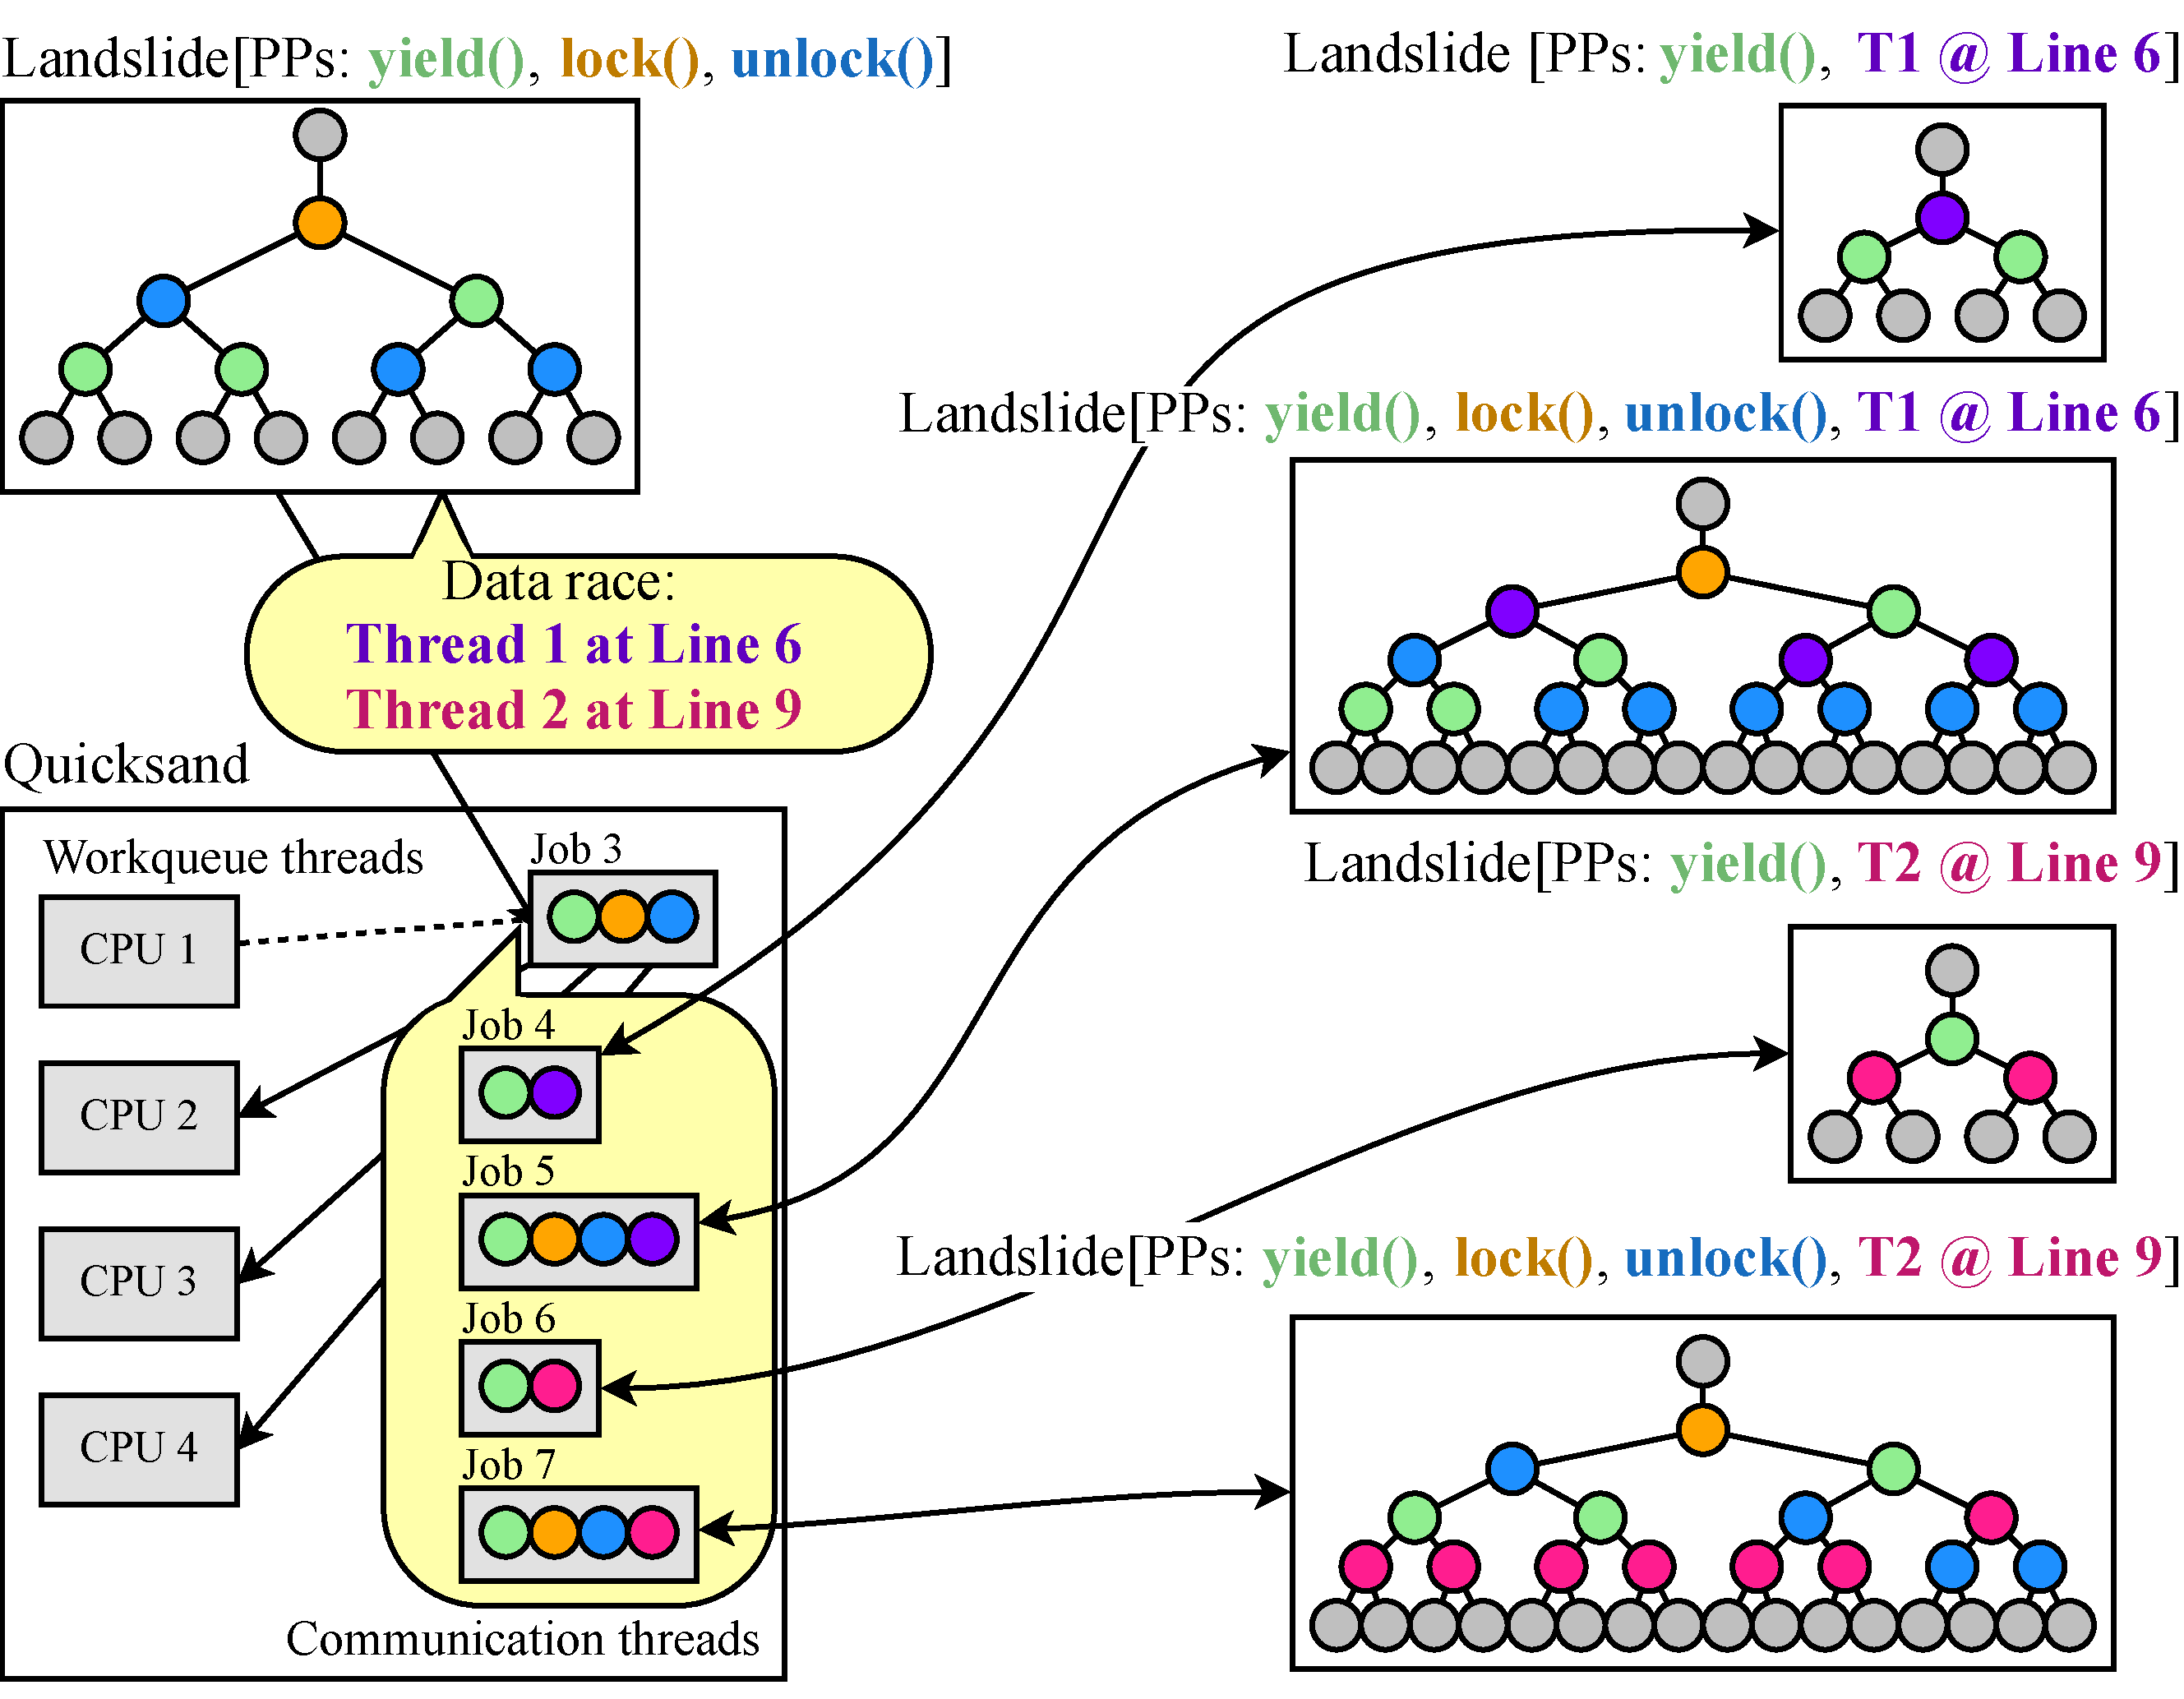
\includegraphics[width=0.9\textwidth]{dr-jobs-v2.pdf}
	\end{center}
	\caption[Quicksand incorporates data races as new preemption points at run-time.]
		{Quicksand incorporates data races as new preemption points at run-time
		by managing the exploration of multiple state spaces,
		communicating with each Landslide instance to receive ETAs, data races, and bug reports.
                %When an access pair is reported as a data race candidate,
                When a data race is reported,
                a new preemption point is added for each involved memory access,
                and new jobs are added for later testing,
                corresponding to different combinations thereof with the existing preemption points.}
        \label{fig:new-dr-jobs}
\end{figure}

The new state spaces may expose a failure, in which case Iterative Deepening must stop and report a data-race bug,
or complete successfully, indicating a {\em benign} (i.e., false-positive) data race.
They may also uncover a new data race candidate entirely in some alternate interleaving,
in which case we may iteratively advance to a superset state space which will preempt at both racing access pairs.
Being constrained by a CPU budget,
Iterative Deepening may time out before completing a data race's associated state space,
in which case the data race remains neither confirmed nor refuted.
%Depending on how much burden the implementation wants to impose on the user,
%it may then report it as a
%report a potential false positive that the user must handle
In such cases, Quicksand elects to impose some burden on the user
by reporting it as a potential false positive
and recommend that she investigate it by hand to judge for herself whether it be a bug.
\cref{sec:quicksand-discussion-partial} will discuss future opportunities for improving
debugging output in cases of such {\em partial verification}.
However, experience shows that this interactivity pays off:
in the next chapter's educational user study (\cref{sec:education-eval}),
one student reported during the survey that they used this recommendation,
combined with their own intuition,
to find a bug that Quicksand was not able to find alone (\cref{sec:education-reasons-worthwhile}).

%%%%%%%%%%%%%%%%%%%%%%%%%%%%%%%%%%%%%%%%%%%%%%%%%%%%%%%%%%%%%%%%%%%%%%%%%%%%%%%%

\subsection{Choosing the best job}
\label{sec:quicksand-choosing}

With a limited CPU budget, many larger tests are likely to be fail to complete in time,
and smaller tests are likely to be more fruitful at finding bugs quickly.
A model checker's state space estimation (\cref{sec:landslide-estimate})
can provide a hint to select between these jobs.
How to handle jobs whose ETAs are too high for the given CPU budget
is the heart of Iterative Deepening,
and is listed formally in \Cref{alg:shouldworkblock}.%
\footnote{
Though its worst-case performance is $O(mn)$ in the
%number of pending and suspended jobs,
sizes of $\mathcal{P}$ and $\mathcal{S}$,
in practice the non-constant portion beyond line~4 runs very infrequently
and is negligible compared to the exponentially-sized state spaces.}.

\begin{algorithm}[t]
	\SetKwInOut{Input}{Input}
	%\textbf{Function} GetBestJob($j_0$, PendingJobs, SuspendedJobs): \\
	\Input{$j_0$, the currently-running job}
	\Input{\PendingJobs, the list of pending jobs, sorted by decreasing heuristic priority}
	\Input{\SuspendedJobs, the list of already-suspended jobs, sorted by increasing ETA}
	\Input{$T$, the remaining time in the CPU budget}
	\If{\GetETA{$j_0$} $<$ HeuristicETAFactor $\times$ $T$}{
		return $j_0$ // Common case: job is expected to finish.
	}
	\ForEach{job $j_P \in$ \PendingJobs}{
		// Don't run a pending job if a subset of it is already suspended; its ETA would be at least as bad. \\
		\If {$\forall j_S \in$ \SuspendedJobs, \GetPPSet{$j_S$} $\not\subset$ \GetPPSet{$j_P$}}{
			return $j_P$
		}
	}
	%// no pending jobs; maybe resume a suspended job \\
	\ForEach{job $j_S \in$ \SuspendedJobs}{
		\If{\GetPPSet{$j_0$} $\not\subset$ \GetPPSet{$j_S$}
			$\land$
			\GetETA{$j_0$} $>$ \GetETA{$j_S$}}{
			// If a subset of $j_S$ is also suspended, don't run the larger one first. \\
			\If{$\forall j_{S2} \in$ \SuspendedJobs, \GetPPSet{$j_{S2}$} $\not\subset$ \GetPPSet{$j_S$}}{
				return $j_S$
			}
		}
	}
	return $j_0$ // \GetETA{$j_0$} was bad, but no other $j$ was better.
	\caption{Suspending exploration of a state space in favor of a potentially smaller one.}
	\label{alg:shouldworkblock}
\end{algorithm}

Its main feature is understanding that if \GetPPSet{$j_1$} $\subset$ \GetPPSet{$j_2$},
and $j_1$ is suspended,
then $j_2$'s state space is guaranteed to be strictly larger, so $j_2$ will take at least as long.
Hence, as long as $j_1$ is suspended on account of being too big,
$j_2$ should not be tested either,
unless $j_1$ is later resumed and its ETA improves over time after further execution.
%reveals that it might finish in time after all.
Similarly, whenever a job finds a bug, all pending superset jobs may safely be cancelled,
as they are guaranteed to contain the same program behaviour, and likely to simply find the same bug again.
%
Implementation-wise,
Quicksand receives an updated estimate from each Landslide instance whenever it finishes executing a new interleaving,
and separates them accordingly
into a set of {\em suspended} jobs,
i.e., partially-explored state spaces with high ETAs,
and a set of {\em pending} jobs,
i.e., untested ones with unknown ETAs.
When Landslide reports an ETA too high for some job,
it is compared with other pending and suspended jobs to find another one more likely to complete in time.%
\footnote{Note that when Quicksand is configured to use multiple CPUs,
simultaneously-running jobs are not considered among the set of possible jbos to switch to,
so if there are fewer total jobs with ETA lower than the time budget than the allowed parallelism factor,
some CPUs may end up speculatively running large jobs
in hopes that the ETA turns out to be an overestimate.}

Iterative Deepening also accounts for the inherent inaccuracy of ETA estimates.
Line~1 heuristically scales up the time remaining to avoid suspending jobs too aggressively
in case their ETAs are actually overestimated.
Lines~12-15 account for the
%bizarre
possibility that among two suspended jobs,
%given two jobs,
%%$j_1,j_2$,
\GetPPSet{$j_1$} $\subset$ \GetPPSet{$j_2$}
but
\GetETA{$j_1$} $>$ \GetETA{$j_2$}.
This may seem surprising,
but can often arise because estimates tend to get more accurate over time,
and $j_1$ perhaps ran much longer, on account of being overall smaller,
before becoming suspended.
In such scenarios,
the algorithm heuristically assumes the smaller job's ETA is more accurate,
in order to avoid repeatedly resuming larger jobs briefly only to find that their ETAs keep getting worse and worse.%
\footnote{In other words, it lets us avoid thrashing in Quicksand.} % ¯\_(ツ)_/¯

%%%%%%%%%%%%%%%%%%%%%%%%%%%%%%%%%%%%%%%%%%%%%%%%%%%%%%%%%%%%%%%%%%%%%%%%%%%%%%%%

\subsection{Heuristics}
\label{sec:quicksand-heuristics}

As predicting the ETAs of state spaces of unknown size
and using that plus size of a set of preemption points as a proxy for how likely a job is to find bugs or complete
is a fundamentally messy process,
it is appropriate to equip the algorithm with some heuristics informed by experience.
\Cref{alg:shouldworkblock} allows the option to heuristically scale a job's ETA
when comparing it to the overall time budget,
which can compensate for any inaccuracy by the estimator.
Quicksand uses a scaling factor defaulting to 2,
chosen based on experiments from prior work \cite{estimation}.
%though we allow changing it via the command line.
It also includes a heuristic to
never suspend jobs before they pass a certain threshold of interleavings tested,
with a default of 32,
informed by my personal experience that ETAs require around that much progress into the state space
before they stabilize (at least relative to each other on similar state spaces,
not necessarily relative to the ultimate true size).%
\footnote{These two heuristics are configurable with the
{\tt -e} and {\tt -E} command-line options, respectively,
as discussed in \cref{sec:landslide-quicksand-options}.}

Landslide classifies data race candidates as {\em both-order} or {\em single-order},
as defined in prior work \cite{portend},
based on whether it observed the racing instructions ordered in both possible sequences or only one
in the original state space, respectively.
Single-order candidates are more likely to be false positives (\cref{sec:background-datarace}),
although preempting during the access itself is necessary to say for sure.
Hence, Quicskand add preemption points for both types of candidates,
and heuristically prioritizes jobs with both-order data races
over those with only single-order data races.
The HeuristicPriority($\alpha$) call in \Cref{alg:handledatarace} corresponds to this strategy.
For single-order races, Quicksand does not initially add a preemption point for the later access at all:
if preempting on the first access is capable of reordering the race,
it will be updated to both-order in the new state space, and the second preemption point will be added then.
\cref{sec:warpzone-heuristics} will discuss opportunities for future work to expand
these heuristics with more nuanced search strategies still.

%%%%%%%%%%%%%%%%%%%%%%%%%%%%%%%%%%%%%%%%%%%%%%%%%%%%%%%%%%%%%%%%%%%%%%%%%%%%%%%%

\subsection{Reallocation false positives}
\label{sec:quicksand-id-realloc}

Finally, I identified a particular class of false positive data race candidates
under the Limited Happens-Before analysis (\cref{sec:background-datarace})
in which the associated memory was recycled by re-allocation between the two accesses,
and claim that it is safe to completely disregard them when considering where to add new preemption points.
\Cref{fig:recycle} shows a common code pattern and interleaving which can expose such behaviour.
If the {\tt malloc} on line~4 returns the same address passed to {\tt free} on line~2,
then lines~1 and 7 will be flagged as a potential data race.
I term this a {\em reallocation false-positive data race candidiate}.
To the human eye, this is obviously a false positive:
reordering lines~4-7 before lines~1-2 will cause {\tt malloc} to return a different region of allocated memory,
in turn causing {\tt x} and {\tt y} to no longer collide.
In studying a similar pattern, the Eraser tool from prior work \cite{eraser}
found that Thread 2's logic usually corresponds to an initialization pattern,
but for generality I have added an arbitrary {\tt publish} action to the example on line~6.

% TODO: fix syntax hilight
% TODO check figure placement
% TODO check figure camption
\begin{figure}[t]
	\begin{center}
	\begin{tabular}{rll}
		& \multicolumn{2}{c}{\texttt{struct x \{ int foo; int baz; \} *x;}} \\
		& \multicolumn{2}{c}{\texttt{struct y \{ int bar; \} *y;~~~~~~~~~~}} \\
		\\
		& {\bf Thread 1} & {\bf Thread 2} \\
		1 & \texttt{\hilight{brickred}{x->foo = ...;}} & \\
		2 & \texttt{\hilight{olivegreen}{free}(x);} \\
		3 & & \texttt{\hilight{commentblue}{// x's memory reallocated}} \\
		4 & & \texttt{y~=~\hilight{olivegreen}{malloc}(sizeof *y);} \\
		5 & & \texttt{\hilight{commentblue}{// ...initialize...}}\\
		6 & & \texttt{publish(y);} \\
		7 & & \texttt{\hilight{brickred}{y->bar = ...;}} \\
	\end{tabular}
	\end{center}
	% TODO: short ver
	\caption{A common execution pattern with {\tt malloc()} that produces false positive data race candidates.}
	\label{fig:recycle}
\end{figure}

As long as the allocation heap is properly synchronized,
a Pure Happens-Before analysis should identify a happens-before edge
between line~2's {\tt free()} and line~4's {\tt malloc()},
and report no race.
However, the upcoming evaluation will show that Limited Happens-Before retains some advantages over Pure
(\cref{sec:quicksand-eval-bugs}),
so it is useful to
%be able to
automatically suppress data race candidates
that are certain to end up being false positives when reordered.
Such collisions could instead be avoided with a hacked allocator which never recycles memory,
but that could unacceptably impact performance in {\tt malloc()}-heavy tests.

The ability to disregard reallocation false positives is unique to Iterative Deepening.
When limited to a single test execution, suppressing any data race candidate matching this pattern is unsound.
Consider the more unusual program in \Cref{fig:recycle-bug},
in which the memory is recycled the same way, but the racing access's address is not tied to {\tt malloc}'s return value.
Here, reordering lines~6-7 before line~3 will allow {\tt x} and {\tt x2} to race.
Discarding the data race report as a false positive after checking just this one execution
would overlook such a bug,
but Iterative Deepening is guaranteed to explore the alternate interleaving,
in which the true data race will show up without {\tt free()} and {\tt malloc()} interposing,
so it is safe to suppress at first, as I will prove in \cref{sec:quicksand-realloc}.
Moreover,
in the context of Iterative Deepening, being able to discard certain data race candidates
allows Quicksand to skip exploring some entire state spaces,
and hence run fewer Landslides overall;
this is analogous to DPOR's ability to skip equivalent interleavings within a single Landslide instance.
Upcoming in the evaluation, \cref{sec:quicksand-eval-verif}'s \Cref{tab:drstatistix}
will show how many redundant state spaces Quicksand is able to prune with this technique.

% TODO smae as above
\begin{figure}[t]
	\begin{center}
	\begin{tabular}{rll}
		& {\bf Thread 1} & {\bf Thread 2} \\
		1 & \texttt{publish(x);} & \\
		2 & \texttt{\hilight{brickred}{x->foo = ...;}} & \\
		3 & \texttt{\hilight{olivegreen}{free}(x);} \\
		4 & & \texttt{x2 = get\_published\_x();} \\
		5 & & \texttt{\hilight{commentblue}{// x's memory recycled}} \\
		6 & & \texttt{y~=~\hilight{olivegreen}{malloc}(sizeof *y);} \\
		7 & & \texttt{\hilight{brickred}{x2->foo = ...;}} \\
	\end{tabular}
	\end{center}
	% TODO: shortver
	\caption{If a single-pass Limited HB analysis discarded candidates matching the malloc-recycle pattern,
it would miss the bug in this adversarial program.}
	\label{fig:recycle-bug}
\end{figure}

%%%%%%%%%%%%%%%%%%%%%%%%%%%%%%%%%%%%%%%%%%%%%%%%%%%%%%%%%%%%%%%%%%%%%%%%%%%%%%%%

\section{Soundness}
\label{sec:quicksand-soundness}

Adding new data-race preemption points in a feedback loop can uncover bugs
not previously reachable by preempting on synchronization APIs alone,
as some prior model checkers do \cite{dbug-ssv},
but how does it compare to the other extreme end of the trade-off,
that is,
committing in advance to preempt on every single shared memory access \cite{spin,inspect}?
It turns out,
assuming sufficient CPU budget,
Iterative Deepening can in principle expose every possible program behaviour that
even that latter approach can find,
providing an equally strong verification guarantee.
This section presents a proof of this claim (\cref{sec:quicksand-convergence}),
as well as a supplementary proof (\cref{sec:quicksand-realloc})
of the soundness of pruning reallocation false positives discussed previously (\cref{sec:quicksand-id-realloc}).

I present these proofs as they appeared in the OOPSLA paper \cite{quicksand}:
written as sketches in informal prose,
to optimize for rapidly conveying an intuition for why it works
rather than to justify every internal step within the proof structure.%
\footnote{Also because I am already over 200 pages in this thesis, all told.}
% footnote yeah, i'm writing this last
% footnote of footnote yeah, the committee never read this part
A more rigorous treatment
is available in the tech report which accompanied the conference paper \cite{quicksand-soundness}.

{\bf Assumptions.}
The proofs are built on a DPOR definition which assumes sequentially-consistent memory hardware.
All algorithms involved are assumed to operate on a machine model of a single globally-consistent execution trace,
which fundamentally cannot account for memory reordering nondeterminism.
%\cref{sec:quicksand-discussion} discusses this limitation further; % that's a lie..
For existing work on combining DPOR with relaxed memory, I refer the reader to \cite{tsopso}.
They also assume the Limited Happens-Before definition
for the data race analysis.
I leave the case for Pure Happens-Before to future work,
although if I may appeal to intuition,
it requires only to show that for any data race candidate
Limited Happens-Before reports in a given execution,
that Pure Happens-Before does not,
either it will be a false positive,
or the latter will find it in an alternate execution within the same state space,
or the latter will find a different data race that ultimately leads to a bigger state space in which the first one may be found,
much like a generalization of \cref{sec:quicksand-realloc}.

\subsection{Convergence to total verification}
\label{sec:quicksand-convergence}

The proof of Iterative Deepening's soundness is in two parts.
In the first part, I prove that for any possible interleaving
one could execute with preemptions anywhere,
an equivalent interleaving must exist using only data-race and synchronization preemption points.
In the second, I prove that starting from synchronization preemption points only,
Iterative Deepening must eventually reach a state space containing such an interleaving,
no matter how many data races are involved.

\subsubsection{Equivalence}

\newcommand\ppnext[1]{\ensuremath{\mathsf{next}(#1)}}
\newcommand\ppinstr[1]{\ensuremath{\mathsf{instr}(#1)}}
\newcommand\ppothers[1]{\ensuremath{\mathsf{others}(#1)}}

Given a preemption point $p$,
let $\ppnext{p}$ denote the next transition after $p$ executed by the thread which ran immediately before $p$,
let $\ppinstr{p}$ denote the first instruction of $\ppnext{p}$,
and let $\ppothers{p}$ denote the transitions by other threads between $p$ and $\ppnext{p}$.

\vspace{0.5em}
\begin{lemma}[Equivalence of non-data-race preemption points]
	For any thread interleaving possible by preempting on any instruction,
	there exists an equivalent interleaving which uses only data-race and synchronization API preemption points.
        \label{lem:relevant}
\end{lemma}

\begin{proof}
Let $p$ be the first preemption point in the given interleaving
such that $\ppinstr{p}$ is not a data race with $\ppothers{p}$ nor is a synchronization API boundary.
Because $\ppinstr{p}$ is not a synchronization boundary,
no lock can be held during $\ppothers{p}$ that was also held by the first thread across $p$.
Hence, because $\ppinstr{p}$ is not a data race, it cannot be a shared memory conflict with $\ppothers{p}$ at all.
Let $i$ be the first instruction among $\ppnext{p}$ which is such a conflict, or a synchronization boundary.
If $i$ is a shared memory conflict, it must be a data race, for the same reasoning as above.
Modify the input interleaving by reordering $\ppinstr{p}$ until $i$, not including $i$, to before $\ppothers{p}$.
By the soundness of DPOR (\cref{sec:landslide-dpor}; \cite{dpor}), this is equivalent to the input interleaving.
In other words, $p$ has been transformed into $p'$ such that $\ppnext{p'} = i$,
which is a data race or synchronization boundary.
All other preemption points in the input trace can be inductively converted in the same manner.
\end{proof}

\subsubsection{Saturation}

For Iterative Deepening to ``eventually'' reach a certain state space,
all data-race preemption points involved must be {\em reachable} during the test.

\vspace{0.5em}
\begin{definition}[Reachability]
	A data race candidate, and its associated preemption point(s),
	are reachable if it will be identified by a model checker
	configured to preempt only on already-reachable preemption points.
\end{definition}
\vspace{0.5em}

Initially, the statically-available synchronization API preemption points (\cref{sec:quicksand-initial-pps})
are reachable.
Reachability of data-race preemption points is transitive.

\vspace{0.5em}
\begin{lemma}[Saturation of data races]
        Given any interleaving comprising only data-race and synchronization API preemption points,
        all involved preemption points are reachable.
        \label{lem:saturation}
\end{lemma}

\begin{proof}
Induct on the preemption points according to the order of their preemptions during an execution sequence.
Given that the interleaving prefix preceding some point $p$ is reachable,
the proof goal is that either $p$ be reachable,
or a new data race among $\ppothers{p}$, not previously reachable, be newly reachable.
The latter condition suffices because in a finitely-sized codebase,
there must be finitely many unique racing instruction pairs.
%, so induction on the number of new data-race preemption points among $\ppothers{p}$ will make $p$ itself reachable.

First, $p$ must be ``coalesced'' away, as well as any other not-yet-reachable points in $\ppothers{p}$.
Consider the alternate interleaving in which the first thread executes past $p$ until the first already-reachable point,
then the other threads among $\ppothers{p}$ execute the same way.
This interleaving's preemption points are all reachable,
so a state space $\mathcal{S}$ containing it will be tested.

If $p$ is a not-yet-reachable data-race preemption point,
it must be possible for some other thread to execute a data-racing instruction with $\ppinstr{p}$.
If this conflict was observed in the state space containing our coalesced interleaving, $p$ is reached.
Otherwise, appeal to the soundness property of DPOR:
%(\cref{sec:landslide-dpor}): % FIXME ugh, this section reference is so handwavy/imprecise
If a program behaviour is possible by interleaving threads at the boundaries of the given transitions,
it will be tested in the containing state space.
By contrapositive, to expose this behaviour,
one or more preemptions must occur in the middle of some transition, rather than at the boundaries.

Let us now see by contradiction that there cannot be {\em multiple} data-race preemption points
which must all be enabled before either data race can be identified;
i.e., a circular dependency.
Assume there does not exist a single transition $t_1 \in \mathcal{S}$
which alone can be split into $\{t_1',t_1''\}$ by a point $q$,
such that another thread's concurrent transition $t_2$ conflicts with $t_1''$.
By the soundness of DPOR, because all $t_2$s are independent with $t_1''$, $\mathcal{S} \equiv \mathcal{S} \cup q$.
Replacing $\mathcal{S}$ with $\mathcal{S} \cup q$ in the above assumption shows that no {\em pair} of new $q$s would expose new program behaviour, and inductively, no set of $q$s of any size, which contradicts the previous paragraph.
%
Hence, a single new not-yet-reachable data race is reachable in $\mathcal{S}$. Hence $p$ will be reached.
\end{proof}

\subsubsection{Convergence}

I name the overall soundness property ``convergence''
in reference to the way it must eventually arrive,
after potentially many iterated state spaces,
at full verification strength.

\vspace{0.5em}
\begin{theorem}[Convergence]
	If a bug can be exposed by any thread interleaving possible
	by preempting on all instructions during a specific test,
	Iterative Deepening will eventually test an equivalent interleaving which exposes the same bug.
        \label{thm:convergence}
\end{theorem}

\begin{proof}
	For any possible interleaving,
	Lemma \ref{lem:relevant} provides an equivalent one with only data-race and synchronization preemption points,
	and Lemma \ref{lem:saturation} proves all involved preemption points are reachable.
	Hence, Iterative Deepening will eventually test a state space containing the equivalent buggy interleaving.
\end{proof}

And thus Iterative Deepening is sound. % :)

\subsection{Suppressing reallocation false positives}
\label{sec:quicksand-realloc}

Next I prove that \cref{sec:quicksand-id-realloc}'s optimization
of discarding reallocation false positives is sound under Iterative Deepening.

\vspace{0.5em}
\begin{theorem}[Soundness of eliminating reallocation data race candidates]
        If a reallocation candidate is not a false positive,
DPOR will reorder threads such that
%DPOR will test an alternate thread interleaving in which
either
the accesses can race without fitting the reallocation pattern,
or a use-after-free bug will be reported immediately.
\end{theorem}

\begin{proof}
Any such program must contain an access $a_1$ by one thread T1,
followed by a {\tt free} and a {\tt malloc} possibly by either thread,
followed by an access $a_2$ by the other thread T2,
not depending on the result of the middle malloc.
Without loss of generality, fix T1 to perform the {\tt free} and T2 the subsequent {\tt malloc},
as shown in \Cref{fig:recycle-bug}.
The other cases are similar,
although note that if T2 performs the {\tt free},
and the {\tt malloc} is reordered before it,
T2's final access will be a use-after-free immediately.
Let us also assume the only way for the program to get pointers to heap memory is through {\tt malloc};
hence, there must also be some ``publish'' action $p$ by T1 which communicates the address to T2.
Because this is a true potential data race,
$p$ must occur before $a_1$, as $a_2$ cannot be reordered before $p$.

The proof goal is that a preemption point be identified during T1 between $p$ and $a_1$.
The publish action must involve some thread communication,
whether through a shared data structure or message-passing API.
If locking or message-passing is used, the set of static synchronization preemption points
(\cref{sec:quicksand-initial-pps})
suffices to provide one.
Otherwise, $p$ (and the corresponding read by T2) will be a potential data race,
although that may itself be another reallocation candidate.
In this case, apply induction on the chain of pointers, if any, leading to the shared address containing $p$:
in the base case, $p$ is communicated via global data or message-passing,
and in the inductive step, DPOR will reorder threads sufficiently to identify a preemption point on $p$.
% the below feels kinda shaky :\ don't remember exactly how this works
% but if someone doubts, they can check out the TR
Note that this induction may result in several possible intermediate preemption points,
each requiring a new state space to be tested,
of course, \Cref{thm:convergence} guarantees this under Iterative Deepening.
Hence there will be a preemption point between $p$ and $a_1$ no matter the mode of communication.

With this preemption point,
DPOR will reorder $a_2$ before $a_1$, while not changing $a_2$'s location.
As T2's {\tt malloc} now occurs before T1's {\tt free}, it will allocate different memory.
Hence $a_1$ and $a_2$ %will be in the same allocation;
can race without appearing to fall under the reallocation pattern.
\end{proof}

This spells QED so we are done \cite{vargomax}. % even more :)))
Note that this proof does not rely on the existence of preemption points on
the internal lock of {\tt malloc} or {\tt free},
which is an ideal candidate to ignore via {\tt without\_function} (\cref{sec:landslide-pps})
to reduce state space size.
Future work may generalize this proof structure to not rely on specific knowledge
of {\tt malloc()}'s and {\tt free()}'s behaviour,
but instead to require only any intervening synchronization event,
thereby extending the overall soundness proof to accomodate Pure Happens-Before as well as Limited Happens-Before.
The experiments in future chapters of this thesis will assume that this holds.

%%%%%%%%%%%%%%%%%%%%%%%%%%%%%%%%%%%%%%%%%%%%%%%%%%%%%%%%%%%%%%%%%%%%%%%%%%%%%%%%
%%%%%%%%%%%%%%%%%%%%%%%%%%%%%%%%%%%%%%%%%%%%%%%%%%%%%%%%%%%%%%%%%%%%%%%%%%%%%%%%
%%%%%%%%%%%%%%%%%%%%%%%%%%%%%%%%%%%%%%%%%%%%%%%%%%%%%%%%%%%%%%%%%%%%%%%%%%%%%%%%

\section{Implementation}
\label{sec:quicksand-implementation}

Quicksand is an independent program that wraps the execution of several stateless model checker instances.
It is expected that Landslide be this checker,
but any other tool which implements the same messaging interface would be compatible as well.
The implementation is roughly 3000 lines of C.
All source files mentioned in this section live in the {\tt id/} subdirectory of the Landslide repository,
with the exception of the Landslide extensions listed last.
As \Cref{chap:landslide} was in some sense a developer's guide to Landslide,
this section will serve similarly for Quicksand.

\subsection{User interface}

The available command-line options for configuring its
CPU-time budget, exploration modes, and so on
are listed in \cref{sec:landslide-quicksand-options}.
Additionally, Quicksand periodically issues a progress report
at fixed intervals to inform the user on the completion, bug-finding, and/or estimated progress of each job.
\Cref{fig:quicksand-progress} shows an example.
I highlight a few notable features of the jobs therein
to serve as a concrete example that may cement the reader's intuition
of \cref{sec:quicksand-id}'s more abstract algorithm descriptions:
\begin{itemize}
	\item Jobs 0, 1, 2, and 3 are the initially-seeded state spaces (\cref{sec:quicksand-initial-pps}).
	\item Job 2 reports a bug found, and shows the filename of the HTML preemption trace
		(\cref{sec:landslide-bugreport}, \Cref{fig:bugreport})
		which the user should examine to diagnose it.%
		\footnote{I actually cheated by copy/pasting this job alone from a different run of Quicksand;
		the other jobs come from a test with the bug already fixed,
		in order that exploration progress far enough to defer some jobs for the sake of example.
		In a real execution, the superset jobs 3, 5, 7, 8, 9, and 11 would be cancelled.}
	\item Jobs 4 and 6 are the ``small'' jobs added to test the two data races in isolation;
		5 and 7 are the corresponding ``large'' jobs (\cref{sec:quicksand-dr-pps}).
	\item Job 11 is the maximal state space, containing all synchronization preemption points
		and both currently-known data races.
	\item The intermediate jobs 8, 9, and 10 have been suspended for having ETAs
		at least twice as large as the provided CPU budget (1 hour),
		according to the ETA scaling factor heuristic (\cref{sec:quicksand-heuristics}).
	\item Note that job 11's ETA is currently lower than 8's, 9's, and 10's, despite being a strict superset of each.
		This corresponds to the surprising ETA inversion situation discussed in \cref{sec:quicksand-choosing}:
		Quicksand simply hasn't made as much progress into job 11 (compare their percentage estimates rather than ETAs)
		for its ETA to be accurate enough yet.
\end{itemize}
Future work could extend these progress reports to be more interactive,
allowing the user to reprioritize state spaces at her whim
or to disable certain data-race preemption points after checking them by hand,
as discussed in \cref{sec:future-friendly}.

% TODO: syn hi
\begin{figure}[t]
	\begin{center}
		\footnotesize
	\begin{tabular}{l}
			% version from buggy run
		%\texttt{==== PROGRESS REPORT ====} \\
		%\texttt{total time elapsed: 40s} \\
		%\texttt{[JOB 0] COMPLETE (4 interleavings tested; 7s elapsed)} \\
		%\texttt{       PPs: \{ \}} \\
		%\texttt{[JOB 1] Running (10.677083\%; ETA 2m 15s)} \\
		%\texttt{       Log: id/ls-output.log.ujrk9U -- PPs: \{ 'mutex\_lock' \}} \\
		%\texttt{[JOB 2] BUG FOUND: landslide-trace-1544661430.29.html (51 interleavings tested; 1 preemptions)} \\
		%\texttt{       Log of lprintf()s: id/ls-setup.log.7UMGLr} \\
		%\texttt{       Log: id/ls-output.log.3Ol8rG -- PPs: \{ 'mutex\_unlock' \}} \\
		%\texttt{[JOB 3] CANCELLED} \\
		%\texttt{       PPs: \{ 'mutex\_lock' 'mutex\_unlock' \}} \\
		%\texttt{[JOB 5] COMPLETE (4 interleavings tested; 7s elapsed)} \\
		%\texttt{       PPs: \{ 'data race 5@ 0x1000ec5' \}} \\
		%\texttt{[JOB 13] Setting up...} \\
		%\texttt{       PPs: \{ 'data race 6@ 0x1000ec5' \}} \\
		%\texttt{[JOB 14] Pending...} \\
		%\texttt{       PPs: \{ 'mutex\_unlock' 'data race 6@ 0x1000ec5' \}} \\
		%\texttt{=========================} \\

		\texttt{==== PROGRESS REPORT ====} \\
		\texttt{total time elapsed: 2m 52s} \\
		\texttt{[JOB 0] COMPLETE (4 interleavings tested; 7s elapsed)} \\
		\texttt{~~~~PPs: \{ \}} \\
		\texttt{[JOB 1] Running (21.932870\%; ETA 8m 14s)} \\
		\texttt{~~~~ PPs: \{ 'mutex\_lock' \}} \\
		% version that came from the actual test
		%\texttt{[JOB 2] Running (46.373457\%; ETA 4m 35s)} \\
		%\texttt{~~~~ PPs: \{ 'mutex\_unlock' \}} \\
		\texttt{[JOB 2] BUG FOUND: landslide-trace-1544661430.29.html (51 interleavings tested)} \\
		%\texttt{~~~~Log of lprintf()s: id/ls-setup.log.7UMGLr} \\
		\texttt{~~~~ PPs: \{ 'mutex\_unlock' \}} \\
		\texttt{[JOB 3] Running (9.852431\%; ETA 24m 32s)} \\
		\texttt{~~~~ PPs: \{ 'mutex\_lock' 'mutex\_unlock' \}} \\
		\texttt{[JOB 4] COMPLETE (6 interleavings tested; 9s elapsed)} \\
		\texttt{~~~~PPs: \{ 'data race @ 0x102917' \}} \\
		\texttt{[JOB 5] Running (3.710938\%; ETA 1h 2m 14s)} \\
		\texttt{~~~~ PPs: \{ 'mutex\_lock' 'mutex\_unlock' 'data race @ 0x102917' \}} \\
		\texttt{[JOB 6] COMPLETE (4 interleavings tested; 8s elapsed)} \\
		\texttt{~~~~PPs: \{ 'data race @ 0x1000ecf' \}} \\
		\texttt{[JOB 7] Running (6.119792\%; ETA 33m 14s)} \\
		\texttt{~~~~ PPs: \{ 'mutex\_lock' 'mutex\_unlock' 'data race @ 0x1000ecf' \}} \\
		\texttt{[JOB 11] Running (3.670247\%; ETA 50m 16s)} \\
		\texttt{~~~~ PPs: \{ 'mutex\_lock' 'mutex\_unlock' 'data race @ 0x102917' 'data race @ 0x1000ecf' \}} \\
		\texttt{[JOB 8] Deferred... (33.340567\%; ETA 2h 6m 3s)} \\
		\texttt{~~~~ PPs: \{ 'mutex\_unlock' 'data race @ 0x102917' \}} \\
		\texttt{[JOB 9] Deferred... (34.466226\%; ETA 2h 35m 37s)} \\
		\texttt{~~~~ PPs: \{ 'mutex\_unlock' 'data race @ 0x1000ecf' \}} \\
		\texttt{[JOB 10] Deferred... (11.113790\%; ETA 4h 20m 31s)} \\
		\texttt{~~~~ PPs: \{ 'mutex\_lock' 'data race @ 0x102917' \}} \\
		% no, i deleted all of them pretending the other data races dont exist
		%\texttt{And 63 more pending jobs should time allow.} \\
		\texttt{=========================} \\
	\end{tabular}
	\end{center}
	\caption{Example Quicksand progress report showing the various possible job states.}
	\label{fig:quicksand-progress}
\end{figure}

Besides the progress reports, Quicksand also prints a notice for each new data race that Landslide detects,
like so, corresponding to the above progress report, for example:
\begin{center}
	%{\tt Found a racy access at 0x0100006f in txn (410user/progs/htm2.c:47)}
	\begin{tabular}{l}
	{\tt Found a racy access at 0x00102917 in deschedule <unknown>} \\
	{\tt Found a racy access at 0x01000ecf in cond\_signal (cond.c:101)}
	\end{tabular}
\end{center}
If using Limited Happens-Before instead of Pure,
it prints ``potentially-racy access'' instead.
This is implemented in {\tt pp\_new()} in {\tt pp.c}.
If the CPU budget runs out and Quicksand must stop exploring prematurely
(or the user's patience runs out and she interrupts it with ctrl-C),
it prints a final report of all data races it was not able to finish classifying as either buggy or benign,
and urges the user to finish checking them with visual inspection
({\tt print\_live\_data\_race\_pps()} in {\tt pp.c}).
It is this feature which one respondent in the student user survey (\cref{sec:education-reasons-worthwhile})
credited for finding an extra bug.

If the verbose option ({\tt -v}) is supplied,
Quicksand will also print one line per interleaving tested by all its Landslide instances,
showing the number of branches tested so far, the estimated percent progress, and the ETA,
as shown earlier in \cref{sec:landslide-estimate}.
This produces a lot more output, and can make progress reports hard to read as they scroll off the screen quickly,
but the author personally finds this mode less disorienting than ten seconds of pure silence between each progress report.
Of course, future work could improve this with a GUI, or at least a split-screen console view.
It will also cause the progress reports to report more detailed information,
such as which preemption points are nondeterministic data races (\cref{sec:quicksand-pps})
and number of reallocation false positives suppressed (\cref{sec:quicksand-id-realloc}).

\subsection{Model checker interface}
\label{sec:quicksand-impl-mc}

The interface with the model checker has two parts.
First, when starting each job, Quicksand creates a configuration file declaring which preemption points to use,
plus other test-case-specific options such as
which preemption points to suppress (\cref{sec:landslide-pps}),
especially those arising from the {\tt malloc} lock (\cref{sec:quicksand-realloc}),
which functions DPOR and data race analysis should treat as trusted code (\cref{sec:landslide-config-landslide}),
whether to enable mutex-testing mode (\cref{sec:landslide-dynamicconfig}),
transactional memory (\cref{sec:tm-implementation}),
and so on.
This is done by {\tt run\_job()} in {\tt job.c}.

Then, a dedicated Quicksand thread
({\tt start\_job()} in {\tt job.c})
communicates with its corresponding model checker process via message-passing
over a FIFO pipe % not gonna cite io.c c.c
({\tt talk\_to\_\allowbreak{}child()} in {\tt messaging.c}).
Landslide messages after testing each interleaving to report updated progress and ETAs
as well as whenever a new data race candidate or bug is found.
Quicksand in turn replies whether to resume/suspend (due to too high ETA) or quit (due to timeout)
({\tt handle\_should\_continue()} in {\tt messaging.c}).
It suspends jobs simply by making Landslide wait on a message-passing reply.
Should Quicksand later re-schedule a suspended job, it sends a message to continue,
resuming Landslide right where it left off;
otherwise, it wakes it up only after time runs out, causing it to exit immediately.
The message-passing format is defined at the top of {\tt messaging.c},
and a matching definition appears in Landslide's source file of the same name.

\subsection{Architecture}

Quicksand's overall architecture is a thread pool of workers,
one for each CPU it was configured to use with {\tt -c} (\cref{sec:landslide-quicksand-options}).
These threads do not correspond directly to each active instance of Landslide,
as some may be deferred;
rather, each worker thread links up temporarily to a job thread, whose duties the previous paragraph describes,
and process them as the overall work-queue of state spaces to be tested demands.
Following is a brief description of each of Quicksand's major modules.

\begin{itemize}
	\item {\bf Job management} ({\tt job.c}):
		Contains the lifecycle code for job threads,
		generation of Landslide configuration files,
		and Linux process management code to launch child Landslide instances ({\tt run\_job()}).
	\item {\bf Messaging} ({\tt messaging.c}):
		Manages communication with child Landslides ({\tt talk\_\allowbreak{}to\_child()},
		implementing certain aspects of Iterative Deepening,
		creating new jobs in response to data race reports ({\tt handle\_data\_race()})
		and deferring too-big jobs in reponse to ETA updates  ({\tt handle\_estimate()}).
	\item {\bf Preemption point registry} ({\tt pp.c}):
		Tracks the set of known synchronization primitives (initialized by main)
		and data races ({\tt pp\_new()}),
		including set comparison routines ({\tt pp\_subset()})
		and computing a job's priority based on the types of included preemption points ({\tt unexplored\_priority()}).
	\item {\bf Workqueue} ({\tt work.c}):
		Implements the per-CPU worker threads,
		including the check for whether to switch priority from one job to another
		(\Cref{alg:shouldworkblock}, {\tt should\_work\_\allowbreak{}block()} and {\tt get\_job()}),
		as well as managing the shared workqueue of jobs overall ({\tt workqueue\_thread()}).
		Also implements the fixed-interval progress reporting ({\tt progress\_report\_thread()}).
	\item {\bf Bugs} ({\tt bug.c}):
		Tracks a list of found bugs for main to repeat at program exit,
		and implements the check for superset state spaces to be cancelled if a subset already found a bug
		({\tt bug\_already\_found()}).
	\item {\bf Options} ({\tt option.c}):
		Processes command-line options,
		checking for legality of various combinations of exploration modes.
		New options may be added with the convenient
		%, if scarily-implemented,
		macros {\tt DEF\_CMDLINE\_FLAG()} and {\tt DEF\_CMDLINE\_OPTION()}.
	\item {\bf Main} ({\tt main.c}):
		Initializes the default state spaces,
		waits for worker threads to terminate after either completion or time-out,
		and issues a final list of bug reports, data race reports, or congratulations as appropriate.
\end{itemize}

Finally, because in very large tests,
the number of suspended Landslide instances may grow without abatement,
Quicksand checks every progress report interval whether the memory footprint of these inactive Landslides
pose a threat to the system's total memory.
Implemented in {\tt cant\_swap()} \cite{cant-stop} in {\tt work.c},
it checks if the system's memory usage exceeds a fixed percentage of its total
({\tt RAM\_USAGE\_DANGERZONE}, default 90),
and if so,
abandons a fixed percentage of suspended Landslides
({\tt KILL\_DEFERRED\_JOBS}, default 50).
%
Generally, the currently-running Landslide instances should never threaten to hit swap,
as there can only be as many of those as CPUs,
but this also accounts for memory used by other processes,
so this is not guaranteed to avoid swapping on a heavily-stressed system
(such as running multiple Quicksands at once).
Naturally, if Quicksand ever needs to invoke this protocol,
any hope at a total verification is compromised.

\subsection{Exploration modes}
\label{sec:quicksand-impl-modes}

In addition to Iterative Deepening,
which Quicksand defaults to if no options are given to specify otherwise,
Quicksand also supports several alternate exploration strategies, as follows.

\begin{itemize}
	\item {\bf Single state space, basic DPOR} ({\tt -C}):
		Runs a single instance of Landslide configured to preempt
		on all statically-known synchronization preemption points.
		Corresponds to dBug's approach \cite{dbug-ssv}.
		Never adds any new preemption points based on data race reports.
	\item {\bf Single state space, ICB} ({\tt -I}):
		Runs a single instance of Landslide with preemption points as above,
		but running Iterative Context Bounding with BPOR (\cref{sec:landslide-icb})
		instead of plain DPOR.
		Corresponds to CHESS's approach \cite{chess}.
		Requires either {\tt -C} or {\tt -M} (see below).
	\item {\bf Single state space, preempt-everywhere} ({\tt -0}):
		Runs a single instance of Landslide as above,
		but preempting on every shared memory access, not just synchronization.
		Corresponds to the approach of SPIN \cite{spin} and Inspect \cite{inspect};
		CHESS supports this mode as well with optional compiler instrumentation.
		Requires {\tt -C}; may optionally be combined with {\tt -I}.
	\item {\bf Maximal state space mode} ({\tt -M}):
		Runs the na\"{i}ve version of Iterative Deepening shown in \Cref{alg:algorithm0},
		i.e.,
		immediately abandons any state space whenever a superset of it exists.
		This results in always testing the maximal state space only, with no inherent parallelism,
		and optimizes for the fastest verification when the user has reason to believe no bugs will exist.
		No prior work implements this approach.
		Note that this mode was implemented after \cite{quicksand}'s publication,
		and I will feature it in the evaluation of transactional memory
		(\cref{sec:tm-eval}) rather than in this chapter.
\end{itemize}

Quicksand restricts ICB to be usable only in modes when it runs only one Landslide at a time.
ICB is itself a heuristic search ordering strategy to uncover bugs faster,
so while technically easy to run Iterative Deepening with all jobs thereunder running ICB,
that would suffer both approaches' repeated work compounded.
\cref{sec:warpzone-heuristics} discusses integrating the two approaches to hopefully reap the benefits of both.
However, maximal state space mode does support ICB,
as it focuses on verification only,
but if the result is a time-out,
the user may find an ICB-style preemption-bounded partial verification useful.

\subsection{Landslide extensions}
\label{sec:quicksand-impl-landslide}

I have added several features to Landslide specifically for use under Quicksand.
Source files mentioned in this subsection live under the usual Landslide source directory.

The other end of the messaging protocol (\cref{sec:quicksand-impl-mc})
is implemented in {\tt messaging.c}.
When Quicksand suspends Landslide,
it detects how much time it spent asleep,
and corrects for that amount during its next ETA computation ({\tt fudge\_time()} in {\tt estimate.c}).
Landslide's data race analysis also includes a heuristic to avoid reporting ``too suspicious''
data race candidates which it believes arise from the initialization pattern \cite{eraser}:
if a conflicting access pair is single-order (\cref{sec:quicksand-heuristics})
and also arose during a known synchronization API's {\tt init()} or {\tt destroy()} function,
Landslide will not message it to Quicksand,
at least not until it is reclassified as both-order.

To recognize the reallocation pattern
discussed in \cref{sec:quicksand-id-realloc}
during data race analysis,
Landslide includes a generation counter in its heap allocation tracking (\cref{sec:landslide-memory}).
Each heap allocation is given a unique ID,
and when evaluating whether two heap accesses can race,
the IDs of their containing blocks must match
({\tt was\_freed\_remalloced()} in {\tt memory.c}),
in addition to the other requirements of Happens-Before.
If the generations do not match,
Landslide sets the {\tt free\_re\_malloc} flag in the messaging protocol to Quicksand.
If the race is later observed in a reordering which avoids the reallocation pattern
(such as in \Cref{fig:recycle-bug}),
Landslide will report it as normal,
and Quicksand will promote it to a normal preemption point in the registry
({\tt pp\_new()} in {\tt pp.c}, ``{\tt for realsies}'' case).
Also included in this message is a flag to indicate whether a data race was found
nondeterministically (i.e., not on the first interleaving), such as described in \cref{sec:quicksand-pps}.

Preempt-everywhere mode (\cref{sec:quicksand-impl-modes})
imposes a heavy burden on Landslide on account of the sheer number of preemption points involved.
First of all, because there are separate tracing entrypoints for memory accesses and instructions ({\tt instrument.c}),
it cannot simply invoke the checkpointing routine (\cref{sec:landslide-timetravel}) immediately.
Also, we must still exclude thread-local and kernel (if testing userspace) or user (if testing kernelspace) accesses.
Rather,
the memory analysis (\cref{sec:landslide-memory}) invokes
{\tt maybe\_preempt\_here()} in {\tt pp.c}
for every access it would ordinary record for DPOR.
If the access is outside of the current stack frame,
and not part of the mutexes (unless {\tt TESTING\_MUTEXES}),
this sets a scheduler action flag {\tt preempt\_for\_shm\_here}
which makes preemption point identification treat it the same as a data race (\cref{sec:landslide-pps}).
{\tt check\_withins()} is also modified to never switch to allowlist mode.
Finally,
Landslide increases its heuristic constant for infinite loop detection (\cref{sec:landslide-infloop})
on the first interleaving from 4000 to $2^{20}$,
to account for the increased orders of magnitude in preemptible events.

%%%%%%%%%%%%%%%%%%%%%%%%%%%%%%%%%%%%%%%%%%%%%%%%%%%%%%%%%%%%%%%%%%%%%%%%%%%%%%%%
%%%%%%%%%%%%%%%%%%%%%%%%%%%%%%%%%%%%%%%%%%%%%%%%%%%%%%%%%%%%%%%%%%%%%%%%%%%%%%%%
%%%%%%%%%%%%%%%%%%%%%%%%%%%%%%%%%%%%%%%%%%%%%%%%%%%%%%%%%%%%%%%%%%%%%%%%%%%%%%%%

\section{Evaluation}
\label{sec:quicksand-eval}

\qrevision{In Quicksand, Iterative Deepening and data race analysis are intimately connected:
the former relies on the later to supply it with new preemption points, thereby refining its search for new concurrent behaviours,
while the latter relies on the former to thoroughly check all possible interleavings around its reported memory accesses and classify them as buggy or benign.
Despite this synergy, which is necessary for total verification soundness (\cref{sec:quicksand-soundness}),
each of these two techniques is a contribution in its own right when it comes to bug-finding performance.
Hence, this evaluation will measure not only the combined approach's full verification power,
but also the bug-finding performance of each technique separately,
as compared to state-of-the-art single-state-space ICB and DPOR.
I pose the following evaluation questions.}

\begin{enumerate}
	\item Does integrating data-race preemption points improve the accuracy of model checking?
		\begin{enumerate}
			\item Do data-race preemption points expose new bugs that couldn't be found with
				synchronization ones alone?
			\item Do data-race preemption points expose the same bugs
				the preempt-everywhere approach could find, faster?
			\item Does Quicksand provide more full verifications %of bug-free programs
				more quickly than the preempt-everywhere approach?
			% not related to new phrasing of Q1, and also the answer is "kinda sorta not really sometimes" anyway
			%\item Does Iterative Deepening find bugs faster in subset state spaces,
			%	even without data-race preemption points?
			\item How does the choice between Pure and Limited Happens-Before
				affect bug-finding and verification performance?
		\end{enumerate}
	\item Does testing alternate interleavings with model checking improve the accuracy of data race analysis?
		\begin{enumerate}
			\item Does Quicksand avoid false positives compared to single-execution Limited Happens-Before?
			\item Does Quicksand find data-race bugs that single-execution Pure Happens-Before or Limited Happens-Before alone would miss?
		\end{enumerate}
\end{enumerate}

\subsection{Experimental setup}
\label{sec:quicksand-expt-setup}

The test suite consists of 79 P2 student thread libraries (\cref{sec:pebbles}),
submitted in 15-410 during the Spring 2014, Fall 2014, and Spring 2015 semesters,%
\footnote{The 2014 semesters were before \Cref{chap:education}'s user study experiments,
and for Spring 2015 (the first semester thereof),
students who used Landslide during the project were excluded from this dataset.}
and 78 Pintos student kernels (\cref{sec:overview-pintos}),
submitted in Berkeley's CS162 and U. Chicago's CMSC 23000 during Spring 2015.
The P2s in this dataset average 1807 lines of C and x86 assembly code,
%, with a standard deviation of 489.5, % i don't know where hte pintos stdev went and i don't wanna recalc it
and the Pintoses average 718 lines (by {\tt diff} to the provided basecode),
for a total of 198,772 lines of code tested for this evaluation.

I chose P2s and Pintoses for this test suite because of the relative ease of generating hundreds of unique state spaces,
varied in size and correctness, and with a diverse set of bug types.%
\footnote{In addition to concurrency bugs,
many of the codebases exhibited {\em deterministic} bugs (i.e., encountered on the first interleaving tested),
which I fixed by hand before running these tests
to ensure that every bug in this study required meaningful work by the model checker.}
While many prior work stateless model checking papers
% TODO: find one that tests like... apache. to back up your claim of realest of the real world
\cite{chess-icb,optimal-dpor,mcr,rcmc}
% bpor could go here but it's already known bugs benchmarks, less the 'real worl' approach
% wow, ZKW15 is 121 programs! nice job!!
publish studies of single-digit or low-double-digit numbers of
bugs found in ``real-world'' programs,
sometimes reported to and confirmed by the upstream developers, %as severe,
to motivate stateless model checking to be used in production settings,
I believe this approach to be too anecdotal for comparing several model checking strategies {\em against each other},
and opt for this approach instead for better statistical significance.%
\footnote{Not to mention -- as I couldn't say in a conference paper, but can say now --
that extending Landslide to support native Linux programs,
complete with filesystem and network nondeterminism,
would have been an engineering burden beyond my ability to do alone and still graduate on time.}

\subsubsection{Test cases}
\label{sec:quicksand-eval-suite}

\newcommand\mxtest{\texttt{mutex\_test}\xspace}
\newcommand\tej{\texttt{thr\_exit\_join}\xspace}
\newcommand\bct{\texttt{broadcast\_test}\xspace}
\newcommand\paraguay{\texttt{paraguay}\xspace}
\newcommand\paradise{\texttt{paradise\_lost}\xspace}
\newcommand\rwldgr{\texttt{rwlock\_downgrade\_read\_test}\xspace}
\newcommand\prisema{\texttt{priority-sema}\xspace}
\newcommand\waitsimple{\texttt{wait-test}\xspace}
\newcommand\alarmsimul{\texttt{alarm-simultaneous}\xspace}

I tested P2s with six multithreaded programs:
\mxtest, for locking algorithm correctness,
\tej, a test of thread lifecycle,
\bct and \paraguay for condition variables,
\paradise for semaphores,
% nb: there used to be a "f u latex" comment here with a \\ after dgr, prob for margins
and \rwldgr for R/W locks.
These are the same tests I distributed Landslide with in \Cref{chap:education};
\cref{sec:education-pebbles-tests} describes them in further detail.
For \mxtest, \paradise, and \paraguay,
I used the {\tt without\_function} command to exclude
{\tt thr\_create()}, {\tt thr\_exit()}, and {\tt thr\_join()} preemption points,
and for \mxtest I enabled {\tt TESTING\_MUTEXES} (\cref{sec:landslide-dynamicconfig}).
I tested Pintoses with three programs from the class's provided test suite:
\prisema, a test of the kernel scheduling algorithm,
\alarmsimul, for the timer sleep routine,
and \waitsimple, for process lifecycle system calls.
These are a subset of those used in \Cref{chap:education}; see \cref{sec:education-pintos-tests}.
Some of the Pintoses were partially implemented,
so each test could only be run on a subset of the 78 submissions;
see the ``Number tested'' column in \Cref{tab:drbugs}.
For all tests,
I also excluded preemption points on {\tt malloc()}'s internal lock using {\tt without\_function}.
In total, the evaluation comprises 629 unique tests (i.e., pairs of a test program and a Pintos or P2),
at least 181 of which will be seen to expose bugs.

\subsubsection{Model checker configuration}
\label{sec:quicksand-expt-trials}

To evaluate the benefits of data-race preemption points and Iterative Deepening separately,
I ran the test suite under Quicksand in three different experimental configurations,
each of which was given a 1-hour budget and 10 CPUs for each test.

\begin{itemize}
	\item {\bf QS-Limited-HB}: Quicksand with Landslide configured to use Limited Happens-Before for its data race analysis ({\tt -H}),
	\item {\bf QS-Pure-HB}: Quicksand using Pure Happens-Before instead ({\tt -V}), and
	\item {\bf QS-Sync-Only}: Quicksand with initial preemption points only,
		as described in \cref{sec:quicksand-initial-pps},
		but never adding new ones from reported data races.
\end{itemize}

I represented the MC State of the Art%
\footnote{The author's DJ name.}
with three configurations of stand-alone Landslide on the same test suite,
corresponding to the search strategies discussed in \cref{sec:quicksand-impl-modes} and \cref{sec:quicksand-impl-landslide}.

\begin{itemize}
	\item {\bf SSS-MC-DPOR}: Single state space mode ({\tt -C})
		using the maximal preemption point set from \cref{sec:quicksand-initial-pps},
		explored with DPOR (\cref{sec:landslide-dpor}),
		%From prior work, dBug \cite{dbug-ssv} implements this approach, among others. %% nb -- already discussed above
        \item {\bf SSS-MC-ICB}: With preemption points as above,
		but instead using ICB \cite{chess-icb} with BPOR \cite{bpor} to find bugs faster
		({\tt -I}, \cref{sec:landslide-icb}), and
		%From prior work, CHESS \cite{chess} implements this approach.
        \item {\bf SSS-MC-Shared-Mem}:
		Using ICB+BPOR, configured to preempt on any shared memory access ({\tt -0})
                (decided at runtime, excluding threads' accesses to their own stacks),
                which in principle includes all possible data races.
		%From prior work, Inspect \cite{inspect} implements this approach,
		%and CHESS also supports this mode with optional compiler instrumentation.
\end{itemize}

Prior work has shown how to parallelize DPOR of a single state space across multiple processors \cite{parallel-dpor},
but it remains an open research problem how to extend the algorithm to ICB.
Hence, I optimistically gave all control experiments a linear speedup of 10 hours per test with 1 CPU;
i.e., assuming it could parallelize with 100\% efficiency.
To match this,
Quicksand reports both the CPU-time and wall-clock time spent during its execution.
Comparing CPU-time leads to a more fair comparison,
although Quicksand's inherent parallelism, which only a wall-clock time comparison would show,
is also a convenient benefit unto itself.
All tests ran on 12-core 3.2 GHz Xeon W3670 machines with 12GB of RAM.

%%%%%%%%%%%%%%%%%%%%%%%%%%%%%%%%%%%%%%%%%%%%%%%%%%%%%%%%%%%%%%%%%%%%%%%%%%%%%%%%

\subsection{Bug-finding}
\label{sec:quicksand-eval-bugs}

\Cref{fig:dowefindbugsfaster-cpu}
plots the bug-finding performance of Quicksand's three experimental trials
against the three control approaches
in a cumulative distribution of total bugs found against elapsed CPU-time.
The farthest-right point on each series indicates in how many total test cases that trial found a bug
after the 10 CPU-hour timeout.
\Cref{fig:dowefindbugsfaster-wall} shows
the same experiments, measured by wall-clock time until each bug was found instead.

\begin{figure}[h]
	\begin{center}
        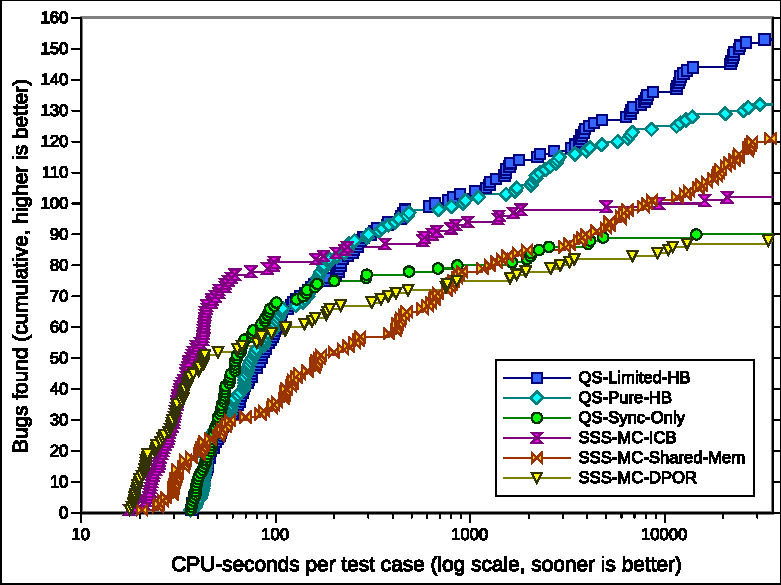
\includegraphics[width=0.9\textwidth]{../proposal/dowefindbugsfaster-v2.pdf} \\
	\end{center}
	\caption[Quicksand's bug-finding performance measured in CPU time.]
		{Quicksand's bug-finding performance measured in CPU time.
		Quicksand finds 125\% as many bugs with data-race preemption points at the 10-hour mark,
		compared to the best prior work approach.
		Quicksand's startup overhead is exaggerated, as the control experiments are not parallelized.}
        \label{fig:dowefindbugsfaster-cpu}
\end{figure}
% TODO: fix placement of the legend in this graph so that it's not awful page back and forthing
\begin{figure}[h]
	\begin{center}
        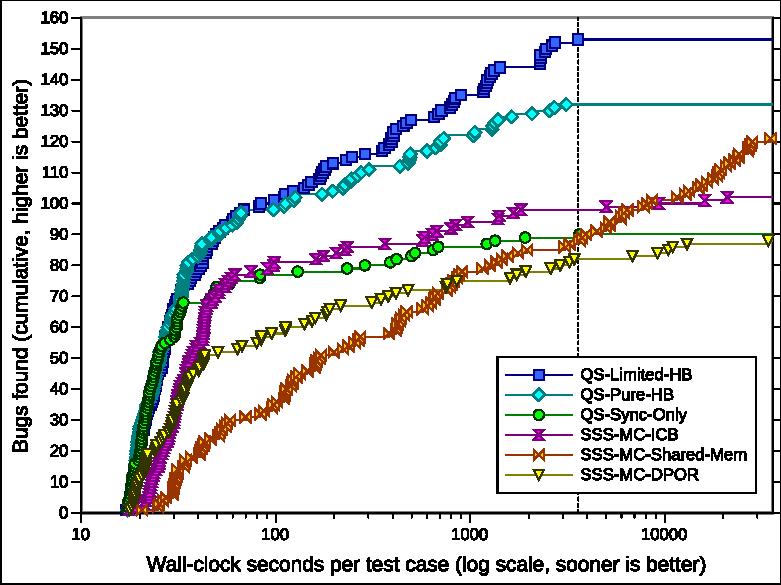
\includegraphics[width=0.9\textwidth]{../proposal/dowefindbugsfaster-wallclock-v2.pdf} \\
	\end{center}
	\caption[Quicksand's bug-finding performance measured in wall-clock time.]
		{Quicksand's bug-finding performance measured in wall-clock time.
		Quicksand is parallelized tenfold; the vertical line indicates its 1 hour limit.}
        \label{fig:dowefindbugsfaster-wall}
\end{figure}

%\begin{figure}[p]
%	\begin{tabular}{c}
%        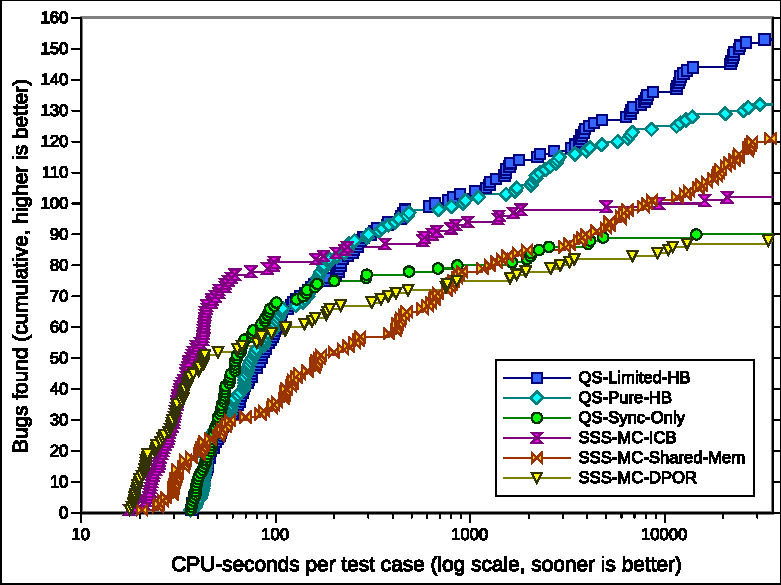
\includegraphics[width=0.71\textwidth]{../proposal/dowefindbugsfaster-v2.pdf} \\
%		\begin{tabular}{p{\textwidth}}
%                (a) Bugs found by Quicksand versus control experiments, measured in CPU time.
%                %as a function of elapsed CPU time.
%                Overall,
%                a more resource-fair comparison than (b),
%                although Quicksand's start-up overhead is exaggerated, as the SSS-MC tests are not parallelized. \\
%		\end{tabular}
%                \\
%                \\
%        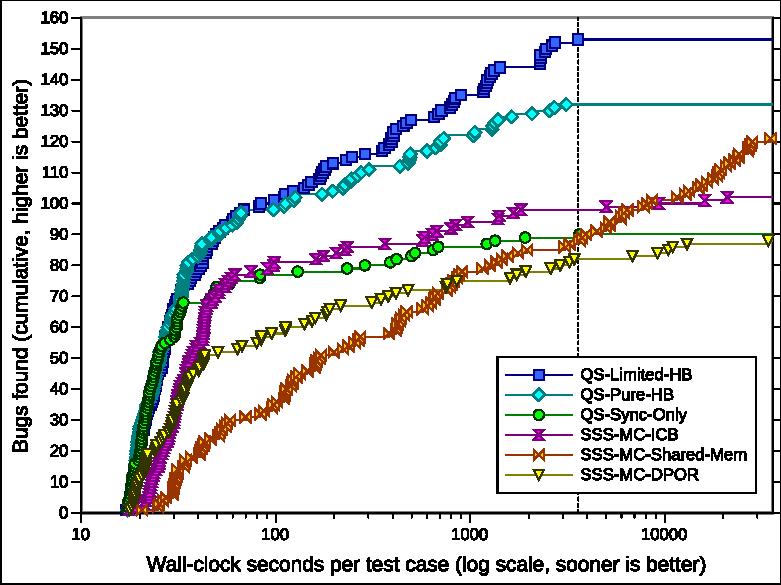
\includegraphics[width=0.71\textwidth]{../proposal/dowefindbugsfaster-wallclock-v2.pdf} \\
%                %(b) Bugs found by elapsed wall-clock time.
%		\begin{tabular}{p{\textwidth}}
%                (b) Bugs found by Quicksand versus control experiments, measured in wall-clock time.
%                Quicksand is parallelized tenfold; the vertical line indicates its 1 hour limit. \\
%		\end{tabular}
%        \end{tabular}
%	\caption[Bug-finding performance comparison
%	between Quicksand and prior work.]
%	{Bug-finding performance comparison between
%        by several configurations of Quicksand and the single-state-space approaches.
%	Quicksand finds 125\% as many bugs
%        with data-race preemption points
%	at the 10-hour mark, compared to the best prior work approach.}
%        \label{fig:dowefindbugsfaster}
%\end{figure}

\subsubsection{Performance comparison}

Compared to SSS-MC-ICB (the fastest among the control experiments),
Quicksand finds more bugs within any fixed CPU budget greater than 200 seconds.
In other words, draw a vertical line at $x=N$ for any $N>200$ to represent timing out each test after $y$ seconds elapsed,
and Quicksand's bug total will exceed that of ICB.
SSS-MC-Shared-Mem initially suffers a substantial performance penalty from the sheer number of preemption points it must analyze,
but ultimately outstrips SSS-MC-ICB, which fundamentally cannot find data-race bugs,
after 135 CPU-minutes with its 100th bug found,
ultimately finishing the 10 CPU-hours as the best prior work approach in the long term.
Compared to SSS-MC-Shared-Mem, Quicksand's Limited HB version
finishes with 125\% as many bugs in total.

Regarding Quicksand's tenfold parallelism,
before the break-even point at 200 seconds,
it lags behind SSS-MC-ICB due to the additional start-up overhead
of testing many state spaces at once even though the easy bugs may be found extremely quickly in any of them.
However, converting ICB's early CPU-time advantage
into faster wall-clock performance remains an open research problem \cite{parallel-dpor}.
\Cref{fig:dowefindbugsfaster-wall} gives Quicksand full credit for its inherent parallelism,
which ICB cannot yet practically match:
with a processor allocation of 10 CPUs, it outperforms all prior work approaches
for any fixed budget of wall-clock time
(i.e., comparing across a vertical line at $x=N$ for any $N$).
% After 1 hour of wall-clock time, tenfold Quicksand performs 158\% as well as SSS-MC-ICB. % totally meaningless

The QS-Sync-Only experiment tests whether Iterative Deepening would be effective
even for model checking domains without data races,
such as distributed systems \cite{macemc,modist,samc,dbug-retreat,concuerror}
and programming languages whose type systems statically reject concurrent mutable shared state
\cite{erlang,haskell,rust-book}.
When Quicksand ignores all data race candidates,
its results are competitive with SSS-MC-DPOR, although SSS-MC-ICB outperforms it slightly.
This is unsurprising: the seed subsets of preemption points
that QS-Sync-Only is limited to
(\cref{sec:quicksand-initial-pps})
are much less flexible than ICB's preemption strategy.
This result suggests that in future work,
Quicksand should consider using ICB in parallel with its default configuration when it finds no data race candidates to test.
I discuss this possibility further in \cref{sec:warpzone-heuristics}.

On the other hand,
comparing QS-Limited-HB to SSS-MC-Shared-Mem
shows that Iterative Deepening thoroughly outperforms ICB when shared-memory preemptions come into play.
%We attribute this to the fact that
Statically configuring a preemption point for every shared memory access in advance
produces orders of magnitude more points than
waiting for an access to be identified as part of a data race at runtime.
%
In principle, DPOR and ICB+BPOR should suffice to identify and prune any equivalent thread interleavings
arising from extraneous preemption points on non-conflicting accesses.
However, in practice,
%we found that
the sheer number of accesses during each new execution
(often thousands)
added significant performance overhead to
%the MC when computing DPOR and backtracking.
DPOR's $O(n^2)$ memory independence computation (\cref{sec:landslide-dpor-conflix}),
as well as the $O(n)$ overhead of checkpointing the execution state at each preemption point (\cref{sec:landslide-timetravel}).
Iterative Deepening avoids this overhead by waiting until runtime
to identify fewer, more relevant preemption points dynamically,
and is hence more suitable for model checking when data races are involved.

\subsubsection{Types of bugs}

\Cref{tab:drbugs} provides more detail on each of the bugs shown in \Cref{fig:dowefindbugsfaster-cpu},
broken down by test case.
The left half shows the number found by each experimental approach,
with the totals of each column corresponding to the values at $x=10$ hours in \Cref{fig:dowefindbugsfaster-cpu}.
In \mxtest, which checks the lock implementation for correctly providing mutual exclusion
(rather than trusting its correctness, as all other tests do),
SSS-MC-ICB and SSS-MC-DPOR
found dramatically fewer bugs (just 1).
Prior work has proposed {\em abstraction reduction} \cite{dbug-phdthesis},
in which verifying correctness properties of synchronization primitives
allows subsequently trusting them in other tests which use them to mitigate state space explosion;
\cref{sec:tm-abstraction} will explore this technique further.
By contrast, QS-Limited-HB found 10 mutex bugs, and SSS-MC-Shared-Mem found 12.
In the scope of this chapter,
this serves as strong evidence that new low-level synchronization code must be verified with data-race preemption points,
whether combined with Iterative Deepening or ICB.

\begin{table}[t]
	\begin{center}
	\small
	\begin{tabular}{r|c||c|c|c|c|c}
		%\multicolumn{2}{c||}{} & \multicolumn{5}{c||}{\bf {Total bugs}} & \multicolumn{4}{c||}{\bf {Data-race bugs}} \\
		% ---
		& {\bf Num.} & \multicolumn{2}{c|}{\bf Quicksand} & \multicolumn{3}{c}{\bf {Single-state-space MC}}
		%& \multicolumn{2}{c|}{\bf {Limited HB}} & \multicolumn{2}{c||}{\bf {Pure HB}} &
		%{\bf Mutual} & {\bf Avg. tested}
		\\
		% ---
		{\bf Test} & {\bf tested} & {\bf LHB} & {\bf PHB} & {\bf ICB} & {\bf DPOR} & {\bf ShMem}
		%& {\bf All} & {\bf Nondet.} & {\bf {All}} & {\bf {Nondet.}}
		%& {\bf timeouts} & {\bf subset SSes}
		\\
		% ---
		\hline
		%         #test qs-lhb qs-phb icb dpor every dronly nondets(LHB) dronly(PHB) nondets(LHB) mutual-TO comp.SSes
		{\tt broadcast\_test}    & 79  & 8   & 8   & 5   & 6   & 7   \\ % & 2 & 1 & {2} & {1} & 7    & 112.3 \\
		{\tt thr\_exit\_join}    & 79  & 23  & 20  & 13  & 13  & 14  \\ % & 11& 4 & {7} & {3} & {12} & {69.7} \\
		{\tt mutex\_test}        & 79  & 10  & 9   & 1   & 1   & 12  \\ % & 9 & 1 & {8} & {1} & 0    & -     \\
		{\tt paradise\_lost}     & 79  & 17  & 16  & 12  & 11  & 12  \\ % & 7 & 3 & {6} & {2} & {50} & {77.4} \\
		{\tt paraguay}           & 79  & 10  & 8   & 5   & 5   & 11  \\ % & 6 & 1 & {3} & {2} & 45   & {59.6} \\
		{\tt rwlock\_downgrade}  & 79  & 27  & 26  & 25  & 23  & 28  \\ % & 4 & 1 & {3} & {0} & {44} & {86.3} \\
		\hline
		{\tt priority-sema}      & 59  & 7   & 7   & 1   & 1   & 8   \\ % & 6 & 4 & {6} & {6} & 2    & 13.0  \\
		{\tt alarm-simultaneous} & 44  & 21  & 12  & 16  & 5   & 29  \\ % & 17& 1 & {7} & {6} & {17} & {7.8}  \\
		{\tt wait-simple}        & 52  & 30  & 26  & 24  & 23  & 1   \\ % & 7 & 2 & {2} & {0} & {15} & {33.8} \\
		\hline
		{\bf Total} & 629 & 153 & 132 & 102 & 88  & 122 \\ % 69& 15& {44}& {21}& {192}& {65.8} \\
	\end{tabular}
	\end{center}
	\caption[Summary of bugs found by each test program.]
	{Summary of bugs
	%and data races
	found by each test program.
	QS-LHB and QS-PHB are Quicksand; ICB/DPOR/ShMem are the controls (\cref{sec:quicksand-expt-trials}).
	}
	\label{tab:drbugs}
\end{table}

To ensure that the corpus of P2 and Pintos bugs gives an unbiased comparison between Quicksand and ICB,
I also counted the preemption bounds at which ICB found each of its bugs,
i.e., the minimum number of involuntary thread switches each bug required to expose.
\Cref{tab:icb-bounds} shows the distribution of these bounds,
which is consistent with the results of \cite[Table 2]{chess-icb},
reproduced in the rightmost column
(obtained under a different test suite, of course, of only 5 programs).
This shows no bias towards bugs that would be harder for ICB to find.
In fact, this evaluation's preemption bound distribution is {\em more} heavily biased towards fewer preemptions,
suggesting that if anything,
my test suite is even friendlier still to ICB than that of prior work.

% TODO: check placement
\begin{table}[t]
	\begin{center}
		\small
	\begin{tabular}{r||c|c||c}
		{\bf Bound} & {\bf SSS-MC-ICB} & {\bf SSS-MC-Shared-Mem} & {\bf Prior work ICB} \cite{chess-icb} \\
		\hline
		0         & 2     & 1     & 3 \\
		1         & 82    & 86    & 7 \\
		2         & 16    & 32    & 5 \\
		3         & 2     & 3     & 1 \\
		4+        & 0     & 0     & 0 \\
		\hline
		\bf Total & 102   & 122   & 16 \\
	\end{tabular}
	\end{center}
	\caption[Distribution preemption bounds among bugs found by ICB.]
	{Distribution of preemption bounds among bugs found by ICB control experiments.
	Bound 0 means the bug was found by switching threads only on {\tt yield} calls.}
	\label{tab:icb-bounds}
\end{table}

%%%%%%%%%%%%%%%%%%%%%%%%%%%%%%%%%%%%%%%%%%%%%%%%%%%%%%%%%%%%%%%%%%%%%%%%%%%%%%%%

\subsection{Verification}
\label{sec:quicksand-eval-verif}

\qrevision{The previous section showed that Quicksand's suite of bug-finding heuristics,
built around Iterative Deepening,
outperform the best single-state-space approaches,
even after correcting
% in a way fair to the state of the art; indeed, {\em unfair} to landslide, by assuming perfect 10x speedup for control expts
for its inherent parallelism.
This section will hold Quicksand to its promise to uphold the other side of the trade-off as well:
that it reach full verification on correct tests reasonably quickly.}

\subsubsection{Full verification}

\Cref{fig:totalverif} plots the cumulative distribution of total verifications provided by each approach,
in the same style of graph as \Cref{fig:dowefindbugsfaster-cpu} and \Cref{fig:dowefindbugsfaster-wall}.
For 167 of the 629 tests,
QS-Pure-HB was able to reach and complete the maximal state space with no bugs found,
hence providing the total verification guarantee justified by the proofs in \cref{sec:quicksand-soundness}.
QS-Limited-HB completed a verification for 153 of 629 tests,
slightly slower on account of Limited Happens-Before's higher false positive rate.
%(which Quicksand must confirm each time by running an extra instance of Landslide). % explained below
The next best approach for verifications was SSS-MC-Shared-Mem, which completed its search in only 39 cases.

\begin{figure}[t]
	\begin{center}
	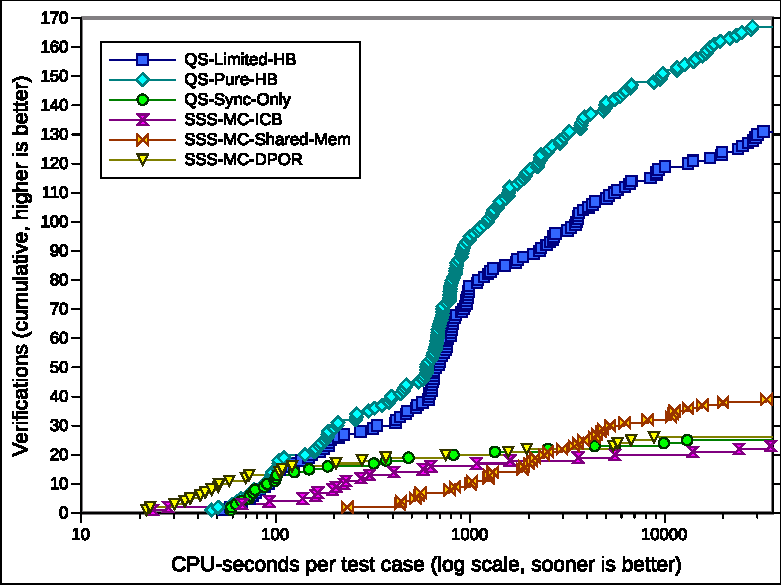
\includegraphics[width=0.9\textwidth]{../proposal/totalverifs-v2.pdf}
	\end{center}
	\caption[Verification performance comparison
	between Quicksand and prior work.]
	{Verification performance comparison between
	Quicksand and single-state-space approaches.
	Among the latter, only SSS-MC-Shared-Mem is theoretically capable of verifying any test with data races;
	the others' series include only tests with no data races whatsoever,
	in which case synchronization preemption points alone suffice for a full verification.}
	\label{fig:totalverif}
\end{figure}

Ultimately, using Limited Happens-Before for finding data race candidates allowed Quicksand to find more bugs,
while Pure Happens-Before allowed for reaching full verification faster.
I attribute this trade-off to the fact that
Limited Happens-Before need not wait to test many alternate thread interleavings before
finding a data race candidate to begin with;
%a potential data race candidate is confirmed;
rather, it can add new jobs to start testing potential races immediately.%
\footnote{Upcoming, \Cref{tab:drstatistix} will corroborate this conclusion:
the difference is most dramatic in {\tt alarm-\allowbreak{}simultaneous},
the test where Quicksand struggled most to finish even small subset jobs.}
%
On the other hand, Limited Happens-Before can get overwhelmed by too many false positives,
needing to refute such candidates by testing new state spaces for each one,
while Pure Happens-Before can refute false positives {\em en passant}
by testing alternate interleavings in its original state spaces.
%In both cases, the performance differences seem to become significant only after about 10 minutes of CPU time,
%which suggests... I don't actually know!
This suggests that
%each approach has merit, and that
model checkers which incorporate data race analysis should implement both modes
and offer the user to choose based on their desired and/or expected testing outcome.

The only testing modes which are theoretically capable of verifying any test with data races
were QS-Pure-HB, QS-Limited-HB, and SSS-MC-Shared-Mem (i.e., preempt-everywhere mode).
When QS-Sync-Only, SSS-MC-DPOR, and SSS-MC-ICB
complete their respective maximal state spaces (i.e., all synchronization preemption points),
that constitutes a full verification only in the case where no data races were identified at all,
meaning Iterative Deepening would search no deeper than that anyway.
Therefore, in \Cref{fig:totalverif},
the data series for these latter three configurations
represent only completed tests with no data races.
Even though SSS-MC-Shared-Mem tends to hang out in the same neighbourhood as them,
note that SSS-MC-Shared-Mem is still steadily increasing in verifications provided at the 10-hour cutoff
(let alone the Quicksand ones),
while the other three seem to reach a plateau of around 20-30 tests relatively soon.

\qrevision{A single-state-space model checker could rely on the user
to properly synchronize all reported data races,
in accordance with the philosophy that even non-failing races should count as bugs
\cite{miscompile-benign,data-races-are-evil},
ultimately improving the number of tests it can verify with no data races.
However, RacerX \cite{racerx} showed that overwhelming the user with warnings about non-failing behaviours
jeopardizes their patience for the tool,
which motivates Quicksand to follow in the footsteps of Portend \cite{portend} instead.}

Overall, including data-race preemption points increases verification capacity by 4.25x.
Assuming sequentially-consistent hardware,
QS-Pure-HB classified many true data races as benign,
while the SSS-MC-ICB approach could at best report such races to the user.
This graph's results show that code written in a natural environment by inexpert users (students)
generally does not obey the sort of strict coding discipline necessary
for a model checker to make simplifying assumptions such as ``no data races'',
justifying this chapter's claim that data-race preemption points are essential to model checking.

\subsubsection{Partial verification}
\label{sec:quicksand-eval-partial}

When a model checking job times out,
the user would more likely prefer a summary of what parts of the test were verified
rather than to write off all the CPU time spent as wasted.
To this end,
Quicksand
%instead
reports which subsets of preemption points resulted in state spaces that did complete in time,
in hopes that the user can supplement such a result with her own intuition
by inspecting the code corresponding to the preemption points not tested (especially data races).
From prior work, Preemption Sealing \cite{sealing}
has argued the value of similar {\em compositional testing} when full verification is intractable,
deferring to the user's expertise to judge the value of each subset of preemption points verified.
\Cref{tab:partialverifs} shows Quicksand's partial verification results on timed-out tests.

\begin{table}[h]
	\begin{center}
	\small
	\begin{tabular}{r|c||c|c}
		% ---
		& {\bf Num.} & {\bf Mutual} & {\bf Avg. tested} \\
		{\bf Test} & {\bf tested} & {\bf timeouts} & {\bf subset SSes} \\
		% ---
		\hline
		%                        #test mutual-TO comp.SSes
		{\tt broadcast\_test}    & 79  & 7    & 112.3 \\
		{\tt thr\_exit\_join}    & 79  & {12} & {69.7} \\
		{\tt mutex\_test}        & 79  & 0    & -     \\
		{\tt paradise\_lost}     & 79  & {50} & {77.4} \\
		{\tt paraguay}           & 79  & 45   & {59.6} \\
		{\tt rwlock\_downgrade}  & 79  & {44} & {86.3} \\
		\hline
		{\tt priority-sema}      & 59  & 2    & 13.0  \\
		{\tt alarm-simultaneous} & 44  & {17} & {7.8}  \\
		{\tt wait-simple}        & 52  & {15} & {33.8} \\
		\hline
		{\bf Total}              & 629 & {192}& {65.8} \\
	\end{tabular}
	\end{center}
	\caption[Summary of partial verification results on timed-out tests.]
	{Summary of partial verification results on timed-out tests.
	``Mutual timeouts'' counts how often both QS-Limited-HB and SSS-MC-ICB
	(the best bug-finding approach from each group)
	timed out. %with no bug found.
	Among those, ``Average tested subset SSes'' counts how many partial verifications
	QS-Limited-HB provided on average for each test. %(\sect{\ref{sec:eval-sssmc}}). % ???
	}
	\label{tab:partialverifs}
\end{table}

On 229 tests, SSS-MC-ICB timed out after 10 hours with no bugs found. % thesis note - pretty sure this *isn't* preempt-everywhere
Among these tests, QS-Limited-HB % thesis note -- i think that's what past-me meant. they just wrote, 'quicksand' but.
found bugs in 37.
The other 192 represent cases where neither Quicksand nor ICB were able to provide a conclusive result either way.
\footnote{Thesis note: SSS-MC-Shared-Mem was added in a subsequent revision to \cite{quicksand}
from when this analysis was conducted, at which time SSS-MC-ICB was the best-performing approach among control experiments.
Nevertheless, mutual timeouts among all six testing approaches constituted roughly one third of the test suite.}
For these 192,
I show the number of state spaces Quicksand was able to complete in the
``Average tested subset SSes'' column.
% of \Cref{tab:drbugs}. % thesis - now split into sep table
%While obviously not as strong as full verification,
These completions guarantee that, if the test program could expose a bug,
it would depend on a data race not discovered yet,
or be reachable only under a superset combination of preemption points not yet reached.

%%%%%%%%%%%%%%%%%%%%%%%%%%%%%%%%%%%%%%%%%%%%%%%%%%%%%%%%%%%%%%%%%%%%%%%%%%%%%%%%

\subsection{Data race analysis}
\label{sec:quicksand-eval-nondets}

Beyond finding new bugs and completing full verifications with data-race preemption points,
I evaluated Quicksand's performance for classifying data race candidates in two ways:
its ability to check nondeterministic data races not reachable under a single-pass analysis (\cref{sec:quicksand-pps})
and its ability to suppress reallocation false positives (\cref{sec:quicksand-id-realloc}).
\Cref{tab:drstatistix} presents the results for this section.

\begin{table}[t]
	\begin{center}
	\footnotesize
	\begin{tabular}{r|c||c|c|c|c||c|c|c||c}
		\multicolumn{2}{c||}{} & \multicolumn{4}{c||}{\bf {Data-race bugs}}
		& \multicolumn{3}{c||}{\bf {Verifications}} \\
		% ---
		& {\bf Num.}
		%& \multicolumn{2}{c|}{\bf Quicksand} & \multicolumn{3}{c||}{\bf {State-of-the-art}}
		& \multicolumn{2}{c|}{\bf {Limited HB}}
		& \multicolumn{2}{c||}{\bf {Pure HB}}
		& \multicolumn{3}{c||}{\bf {Pure HB}}
		& \multicolumn{1}{c}{\bf {Realloc.}}
		\\
		% ---
		{\bf Test} & {\bf tested}
		%& {\bf LHB} & {\bf PHB} & {\bf ICB} & {\bf DPOR} & {\bf ShMem}
		& {\bf All} & {\bf N.D.} & {\bf {All}} & {\bf {N.D.}}
		& {\bf DR PPs} & {\bf Benign} & {\bf Untested} & {\bf FPs} \\
		% ---
		\hline
		%                      #test dronly nond dronly nond
		%                                                   drpps benign untest FRMs
		{\tt broadcast\_test}    & 79  & 2 & 1 & {2} & {1} & 655  & 97  & 150 & 52  \\
		{\tt thr\_exit\_join}    & 79  & 11& 4 & {7} & {3} & 566  & 68  & 249 & 338 \\
		{\tt mutex\_test}        & 79  & 9 & 1 & {8} & {1} & 911  & 127 & 44  & 7   \\
		{\tt paradise\_lost}     & 79  & 7 & 3 & {6} & {2} & 783  & 2   & 414 & 166 \\
		{\tt paraguay}           & 79  & 6 & 1 & {3} & {2} & 936  & 9   & 510 & 180 \\
		{\tt rwlock\_downgrade}  & 79  & 4 & 1 & {3} & {0} & 543  & 1   & 310 & 156 \\
		\hline
		{\tt priority-sema}      & 59  & 6 & 4 & {6} & {6} & 65   & 51  & 3   & 0   \\
		{\tt alarm-simultaneous} & 44  & 17& 1 & {7} & {6} & 35   & 0   & 29  & 35  \\
		{\tt wait-simple}        & 52  & 7 & 2 & {2} & {0} & 71   & 1   & 28  & 31  \\
		\hline
		{\bf Total}              & 629 & 69& 15& {44}& {21}& 4565 & 356 & 1737& 965 \\
	\end{tabular}
	\end{center}
	\caption[Data race statistics among Quicksand experiments.]
	{Data race statistics among Quicksand experiments.
	``Data-race bugs'' counts, among Quicksand's bugs, how many required data-race preemption points to expose;
	among those, the ``N.D.'' (``nondeterministic'') columns show how many candidates
	required model checking to identify
	in the first place
	(\cref{sec:quicksand-eval-nondets}).
	%
	``Total DR PPs'' counts how many unique data-racing instructions
	QS-Pure-HB identified among tests where it found no bugs.
	Among those, ``Benign'' counts how many were refuted as non-failing,
	while ``Untested'' counts how many could not be checked in the time limit.
	Finally, ``Realloc. FPs'' counts how many reallocation false positives QS-Limited-HB suppressed.
	}
	\label{tab:drstatistix}
\end{table}

\subsubsection{Nondeterministic data races}

Some memory accesses may be hidden in a control flow path that requires a nondeterministic preemption to be executed
(\cref{sec:quicksand-pps}).
In such cases, a single-pass dynamic data race detector
might not achieve the coverage necessary
to identify a racing access pair as a candidate at all,
let alone check the resulting behaviour with such as Landslide.
I instrumented Landslide to report these to Quicksand
and counted how many such led to Quicksand finding new bugs when used as preemption points.
Such bugs could be considered {\em false negatives} of the single-pass approach.
The left half of \Cref{tab:drstatistix}
breaks down the types of bugs
found in each test case,
showing both the total number of data-race bugs
and the number among those that required such nondeterministic data races to expose.
% I denote these data race reports as {\em nondeterministic},
% while those that could be found on the first interleaving .....
%
To ensure a fair comparison, I disabled Quicksand's reallocation false positive suppression
(\cref{sec:quicksand-id-realloc}, itself evaluated in the next section)
for this experiment.
This prevents Landslide from suppressing an observed reallocation data race candidate on the first interleaving,
which would falsely classify it as nondeterministic,
even though a single-pass would not (indeed, should not) suppress such candidates.

\Cref{fig:dr-falsenegs}
%compares the types of data race candidates necessary to expose each data-race bug in the test suite.
visualizes the difference between single-pass and model-checking-enabled data race analysis.
The first and third series represent the bugs found using preemption points from single-pass data race candidates only,
% not entirely true, as portend could be given data race traces from an MC
%but they don't do it in their paper, so i feel comfortable making this claim
i.e., the state-of-the-art approach used by RaceFuzzer \cite{racefuzzer} and Portend \cite{portend}.
The second and fourth series show all data-race bugs Quicksand found,
which includes the former type as well as new bugs involving nondeterministic races.
QS-Limited-HB found a nice 69 data-race bugs in total, % nice
15 of which %could not be found with single-pass data race candidates alone.
required nondeterministic data-race preemption points to expose.
QS-Pure-HB is even more dependent thereupon, %on nondeterministic data-race preemption points,
%requiring nondeterministic data-race preemption points
requiring them in 21 cases among its 44 total data-race bugs.
Moreover, although the frequency
of these nondeterministic races varies across the different test cases
(for example, almost all in {\tt broadcast\_test} were nondeterministic; almost none in {\tt mutex\_test}),
they are still at least present in all tests,
meaning it is not just an issue of writing ``better'' test cases to avoid them.

\begin{figure}[t]
	\begin{center}
	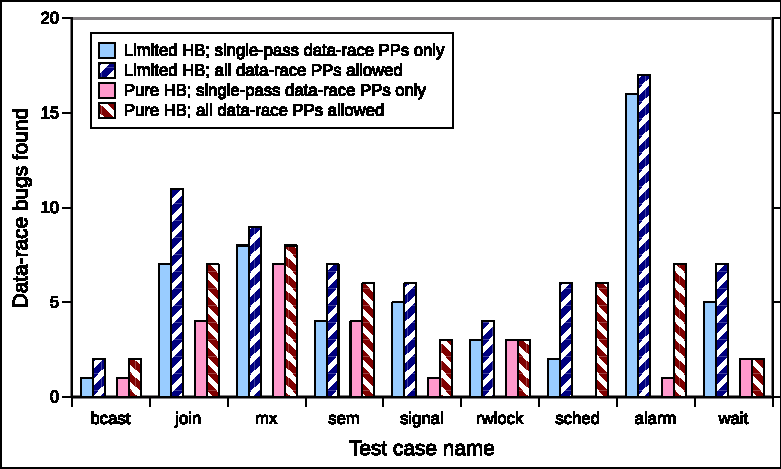
\includegraphics[width=0.9\textwidth]{../proposal/nondets.pdf} % TODO: get some gf colors on here
	\end{center}
	\caption[Nondeterministic data-race preemption points are required to find some bugs.]
	{Nondeterministic data-race preemption points are required to find some bugs.
	Requiring stateless model checking integration to identify to begin with,
	incorporating these races as new preemption points
	allowed Quicksand to find
	% lhb: 127.77%
	% phb: 191.30%
	128\% (Limited HB) to 191\% (Pure HB) as many data-race bugs
	compared to using single-pass candidates alone.
	}
	\label{fig:dr-falsenegs}
\end{figure}

Note that I do not compare how much testing time is required before identifying the data races %candidates
involved in each bug.
While single-pass data races are all found after a single test execution,
Quicksand may potentially take up to all 10 CPU-hours before identifying a nondeterministic data race.
However, prior work data race tools \cite{tsan,fasttrack},
being not integrated with a model checker,
are not intended to discover new candidates under subsequent runs.
Running a single-pass data race tool repeatedly for 10 CPU-hours could potentially uncover some nondeterministic candidates,
but stress testing's comparative problem with achieving reliable coverage is already well-understood
\cite{chess-icb,gambit},
so I hope the reader will consider this experiment enough evidence for model checking already.
Likewise, replay-based tools such as RaceFuzzer \cite{racefuzzer} and Portend \cite{portend}
depend upon the data race detector to provide an execution trace leading to each candidate.
This result suggests that
such tools could benefit from a similar feedback loop as is used in Iterative Deepening,
for example, to discover new transitively-reachable data races while testing initial ones,
even if full verification not necessarily be their goal.

\subsubsection{Reallocation false positive suppression}

In \cref{sec:quicksand-realloc} I showed the soundness of
suppressing data race reports between two heap accesses when the surrounding memory was re-allocated in between.
\Cref{tab:drstatistix}'s ``Realloc FPs'' column shows the total number of such data race candidates for each test program,
totaling 965 across all tests.
% NB. Calculated this by grepping QS-LHB id-logs for "for realsies" (see quicksand pp.c).
Among these, only 64 were observed to avoid the reallocation in an alternate interleaving,
thereupon being promoted to real data-race preemption points.
\cref{sec:quicksand-realloc}'s proof guarantees the safety of pruning all state spaces resulting from the 901 others.
%
Among the 64 true data races, %which initially fit the malloc-recycle pattern,
none exposed a new bug when used as a preemption point.
This suggests that for other data race tools,
suppressing reallocation candidates may be a productive heuristic,
even if unsound without Iterative Deepening.
However, Quicksand was able to correctly identify the 64 violations of that heuristic, among 26 distinct tests,
and fall back to classifying them with DPOR.

%%%%%%%%%%%%%%%%%%%%%%%%%%%%%%%%%%%%%%%%%%%%%%%%%%%%%%%%%%%%%%%%%%%%%%%%%%%%%%%%
%%%%%%%%%%%%%%%%%%%%%%%%%%%%%%%%%%%%%%%%%%%%%%%%%%%%%%%%%%%%%%%%%%%%%%%%%%%%%%%%
%%%%%%%%%%%%%%%%%%%%%%%%%%%%%%%%%%%%%%%%%%%%%%%%%%%%%%%%%%%%%%%%%%%%%%%%%%%%%%%%

\section{Discussion}
\label{sec:quicksand-discussion}

This section will list the current limitations of Quicksand and Iterative Deepening
and discuss opportunities for future improvement.

\subsection{Experimental bias}

\qrevision{The evaluation design (\cref{sec:quicksand-expt-trials})
contains two major shortcomings
that, to my surprise, no conference reviewer, audience member, or colleague ever called me out on.
Firstly, the single-state-space preempt-everywhere
strategy was conducted only with ICB enabled (SSS-MC-ShMem).
This resulted in reasonable bug-finding performance,
ultimately reaching 80\% as many bugs found as Quicksand's best (QS-Limited-HB) in \Cref{fig:dowefindbugsfaster-cpu}.
However, ICB tends to repeat work across multiple preemption bound iterations, %hurts its overall completion time,
as evidenced between SSS-MC-ICB and SSS-MC-DPOR in \Cref{fig:totalverif}.
Correspondingly, a version of SSS-MC-ShMem configured to use traditional DPOR without ICB would
effectively begin with a preemption bound of infinity
and perhaps be more competitive with Quicksand on verifications.
%by avoiding ICB's tendency to repeat interleavings. %across iterations.
Of course, this would trade off against its bug-finding performance,
but an expert user could compensate by deciding between the two modes
depending whether she thinks the test is more likely to be buggy or correct.
Granting such user involvement,
Quicksand's maximal state space mode (\cref{sec:quicksand-impl-modes})
would correspondingly verify more tests than QS-Pure-HB, %within those 10 CPU-hours,
especially if it were given 10 wall-clock hours on 1 CPU rather than 1 on 10.
Future work could also improve both Quicksand's and ICB's ability to identify and skip redundant work
across their respective iterations,
as discussed below.

Secondly, and more fundamentally, representing state-of-the-art approaches by reimplementing them in one's own tool is fraught.
The comparison between Iterative Deepening and ICB in
\cref{sec:quicksand-eval-bugs} and \cref{sec:quicksand-eval-verif}
could possibly be conflated by Landslide's implementation of ICB and/or DPOR being slower
on account of the simulated execution environment (\cref{sec:landslide-architecture}).
A more rigorously scientific comparison would extend a prior work model checker, such as CHESS \cite{chess},
to support dynamically-configured data-race preemption points,
and evaluate Quicksand with it versus its own ICB implementation as well,
to isolate any such conflating factors.
Concurrently with these results' publication in OOPSLA \cite{quicksand},
more advanced state space reduction algorithms were proposed, such as Maximal Causality Reduction (MCR) \cite{mcr}.
It is not immediately obvious that MCR's benefit would be orthogonal with Iterative Deepening;
i.e., the benefit of Quicksand with a MCR-enabled model checker might be reduced
compared to the benefit shown in \cref{sec:quicksand-eval-bugs} and \cref{sec:quicksand-eval-verif}.
Future comparisons of model-checking strategies should strive to reach these higher bars of scientific rigor.}

\subsection{Avoiding redundant work}

When Quicksand extends a small state space with more preemption points,
the new state space is guaranteed to test a superset of interleavings compared to the old one.
Because Quicksand prioritizes completing small state spaces before their descendants,
the superset state spaces we run later will repeat each branch of their already-completed subsets,
and any interleaving which does not preempt threads on any of the new preemption points will be repeated work.
%
% lol i never did this
%We measured the proportion of repeated work among completed state spaces across our test suite;
%on average, {\bf \large 999\%} of the interleavings in each test were repeated, with some tests as high as {\bf \large 9999\%}.
This may make Quicksand slower than the single-state-space approach to find certain bugs,
for example, if both {\tt mutex\_lock()} and {\tt mutex\_unlock()} preemption points
together expose a bug, but not either alone.
Predicting whether an upcoming interleaving has already been tested is not straightforward,
but future implementations
of Iterative Deepening and/or ICB
could incorporate cross-job memoization
to prune some or all such repeated work.

Similarly, when pursuing total verification,
if the state space resulting from preempting on every instruction
(or equivalently, the maximal state space, thanks to \cref{sec:quicksand-soundness})
could be completed in time,
a model checker which immediately jumped to that state space,
abandoning all smaller subsets would certainly achieve verification faster.
Quicksand's maximal state space mode ({\tt -M}, see \cref{sec:quicksand-impl-modes})
can strike a middle ground between Iterative Deepening and single-state-space preempt-everywhere,%
\footnote{Thesis note: {\tt -M} mode was implemented after the conference paper's publication \cite{quicksand},
and will be evaluated alongside transactional memory later in \cref{sec:tm-eval}.}
but future implementations of Iterative Deepening could prioritize the maximal state space more flexibly still.
For example, pinning its job to one of the available processors regardless of the status of any smaller jobs
would avoid getting too flooded with smaller jobs to even begin the maximal job before time runs out.
When full verification is infeasible,
completing even an intermediate-sized job would allow immediately pruning all subset jobs thereof,
perhaps using a form of binary search (on the preemption point set size) to find an appropriately-sized intermediate job.

\subsection{Preemption point subsets}
\label{sec:quicksand-discussion-subsets}

Quicksand was able to partially guarantee safety for some preemption points
in 93\% of tests with too-large maximal state spaces (\cref{sec:quicksand-eval-partial}).
However, in 6 cases, no more than the minimal state space could be verified,
and in 18 others, no state spaces were completed at all.
Larger state spaces often result from finer-grained locking,
which can indicate a more intricate concurrent algorithm or an unnecessarily complicated design (or both).
Such programs may require even more rigorous verification than a program with a single global lock,
making them important to consider for future work.
While Quicksand uses {\tt within\_function} (\cref{sec:quicksand-impl-mc})
{\em statically} to restrict where preemption points could arise in advance of the test,
future
Iterative Deepening
implementations could use this mechanism to {\em dynamically} subset preemption points further,
making partial verification of larger tests possible,
potentially even involving the user with interface options
to enable and disable preemption points of her choosing at run-time.
\cref{sec:warpzone-heuristics} discusses this possibility further.

\subsubsection{Static data race analysis}

In \cref{sec:quicksand-eval-bugs}, I evaluated the state-of-the-art approach's ability to find data-race-induced failures
by configuring a static predicate to preempt on any non-stack memory access
({\tt -0}, see \cref{sec:quicksand-impl-modes}).
This introduced hundreds of new preemption points on each new test execution,
with a prohibitive performance impact.
While this performance could be improved by
relaxing the preemption strategy,
instead using a static or single-pass analysis to find data race candidates in advance \cite{portend},
that would sacrifice soundness of the verification guarantee, as I showed in \cref{sec:quicksand-eval-nondets}.
However, Quicksand itself could employ static data race analysis such as RacerX \cite{racerx},
or single-pass dynamic analysis such as ThreadSanitizer \cite{tsan} in future work.
% These tools tend to err on the side of false positives,
% but also include .....
Any data race candidates identified in advance could heuristically be included in Quicksand's initial seed preemption point sets
(\cref{sec:quicksand-initial-pps}),
enabling it to focus on the most suspicious races immediately,
rather than waiting for them to be identified after potentially many iterations of model checking.

\subsection{Partial verification}
\label{sec:quicksand-discussion-partial}

% Likewise,
When full verification is not computationally feasible,
some jobs with data-race preemption points will inevitably time out,
and Quicksand cannot guarantee those races are
false positives or
benign, even though no bug was found.
In the ``Untested DR PPs'' column of \Cref{tab:drstatistix},
I show how many such candidates Quicksand (with Pure Happens-Before) could not verify in each test,
ultimately totaling 38\% of all data races in tests which timed out.
In prior work,
Portend introduced the {\em k-witness harmless} metric \cite{portend}
for heuristically classifying the likelihood that each data race lead to a failure or be benign.
Quicksand could incorporate this metric to guide the user's attention
to the unverified data races most likely to be worth her time.
%
In \cref{sec:quicksand-eval-partial} I presented partial verification results
measured in tens or hundreds of subset state spaces completed on average per test case.
However,
%On the other hand,
attempting to maximize the raw number of completed state spaces
is not necessarily the most user-friendly way to present partial verifications.
For starters, those numbers included small state spaces which were subsets of other state spaces also completed;
the user need not examine both subset and superset separately to understand what was tested.
Future work should at least perform basic set comparisons
to present only the non-redundant state spaces completed when time runs out.
For a further research challenge,
user studies could help to determine the most effective interface for presenting these partial results
from a software development perspective,
which I discuss further in \cref{sec:future-friendly}.

Quicksand is not the first concurrency tester to provide a partial verification guarantee
when it times out on too-large tests.
Probabilistic Concurrency Testing (PCT)
\cite{randomized-scheduler}
proposes to use random exploration of the state space and quantify the probability
that a bug may remain in some untested interleaving after a time-out,
eschewing DPOR's depth-first search model to
instead sample broad cross-sections of large state spaces.
However, it proposes no alternate reduction strategy, making full verification impractical,
and furthermore is opaque to the user about which parts of her code were actually tested.
Meanwhile, ICB proposes to inform the user
of the maximum number of preemptions used to test any individual interleaving,
under the assurance that most bugs are likely to be found with fewer preemptions (\Cref{tab:icb-bounds}).
Iterative Deepening
%offers a clear benefit to the expert user
%via the {\tt within\_function} command,
%which enables her
allows the expert user
to restrict a test's scope via the {\tt within\_function} command to only the modules of a codebase she wishes to test.
These guarantees could each be useful to developers in different scenarios,
and future work could combine the three approaches to provide all benefits at once,
for example, using ETAs to heuristically decide when to switch between DPOR, ICB, and/or PCT in large state spaces,
as discussed further in \cref{sec:warpzone-heuristics}.

%%%%%%%%%%%%%%%%%%%%%%%%%%%%%%%%%%%%%%%%%%%%%%%%%%%%%%%%%%%%%%%%%%%%%%%%%%%%%%%%
%%%%%%%%%%%%%%%%%%%%%%%%%%%%%%%%%%%%%%%%%%%%%%%%%%%%%%%%%%%%%%%%%%%%%%%%%%%%%%%%
%%%%%%%%%%%%%%%%%%%%%%%%%%%%%%%%%%%%%%%%%%%%%%%%%%%%%%%%%%%%%%%%%%%%%%%%%%%%%%%%

\section{Summary}

\qrevision{In order to supplant conventional stress testing,
which, despite its
%tendency to overlook subtle and severe nondeterministic bugs,
%lack of any formal coverage guarantees,
inability to reliably expose, reproduce, or verify absent bugs in any finite amount of testing time,
remains a popular choice for concurrency programmers of all skill levels,
stateless model checking must meet users' needs regarding realistic testing budgets.
This chapter has presented Quicksand, which automatically navigates the trade-off
between fast bug-finding and formal verification depending on the size of the test.
My contributions have been as follows.

\begin{itemize}
	\item Iterative Deepening (\cref{sec:quicksand-id}),
		an algorithm for model checkers to simultaneously test multiple state spaces,
		incorporating new preemption points identified with dynamic analysis on the fly.
	\item A proof of convergence (\cref{sec:quicksand-convergence}),
		showing that for any verification obtained under even the most extreme preemption strategy,
		Iterative Deepening with data race analysis provides an equivalently strong one,
		with far fewer preemption points necessary.
	\item A technique for suppressing certain false positive data race candidates % TODO: hm, should false-positive be hyph?
		under Limited Happens-Before (\cref{sec:landslide-lhb})
		by identifying intervening {\tt malloc()} and {\tt free()} calls
		(\cref{sec:quicksand-id-realloc}),
		and a corresponding soundness proof when this technique is used under Iterative Deepening
		(\cref{sec:quicksand-realloc}).
	\item Quicksand (\cref{sec:quicksand-implementation}),
		an Iterative Deepening implementation which incorporates several heuristics for prioritizing
		which state spaces are most likely to uncover bugs % this claim is not scientifically justified
		or, should no bugs exist therein,
		which ones are most likely to complete within a user-specified fixed CPU budget,
		as informed by state space estimation (\cref{sec:landslide-estimate}).
	\item A 629-test evaluation of Quicksand
		against several prior state-of-the-art model checking approaches implemented in Landslide
		(\cref{sec:quicksand-eval}),
		which showed that Quicksand provides both faster bug-finding (\cref{sec:quicksand-eval-bugs})
		and more full verifications (\cref{sec:quicksand-eval-verif}),
		delivering ``the best of both worlds'' as promised,
		and also demonstrated the need for a bidirectional feedback loop
		between model checking and data race analysis
		(\cref{sec:quicksand-eval-nondets}).
\end{itemize}

The next chapter will tell of my experience and results deploying Landslide in an educational setting,
equipped with Quicksand to allow even inexperienced student users to benefit from stateless model checking
with little to no manual configuration burden.}

\chapter{Education}
\label{chap:410}

This chapter proposes my plan to evaluate Landslide's effectiveness as a debugging aid for students in an educational setting.
This is the second of the three projects I am proposing for this thesis, and is currently ongoing work.
What remains to be done is detailed in Section~\ref{sec:grading}.

\section{Motivation}

In my MS thesis \cite{landslide}, I solicited students at CMU's Operating Systems Design and Implementation class
(henceforth, ``15-410'')
to volunteer at the end of the P3 project to annotate their kernels and try debugging them with Landslide.
However, the annotation burden undermined Landslide's purpose:
the only students willing to spend free time on manual instrumentation were biased to be those who were already doing well in the class,
and hence least likely to benefit from Landslide's debugging potential.
(Actually, even the best 15-410 students still have concurrency bugs,
but in principle, an educational tool must reach the more struggling students,
the so-called ``middle'' and/or ``bottom'' of the class.)
%
Requiring annotations hurts Landslide's case as a grading tool, as well:
TAs need to understand the kernel to begin with in order to annotate correctly,
and while achieving such understanding they may as well grade it by hand, as before.

Since then, I've extended Landslide to support testing P2 thread libraries (Section~\ref{sec:pebbles}) as well.
Because P2 mandates specific function names for the project's internal APIs
-- most importantly, for the concurrency primitives --
Landslide can automatically annotate arbitrary student implementations with no manual effort required of the user (whether student or TA).
The addition of Quicksand and Iterative Deepening (Chapter~\ref{chap:quicksand}) partly fulfills this purpose,
freeing student attention from the issue of which state spaces to test.
This chapter will detail my further techniques and evaluation which are specific to educational use.

\section{Implementation Details}

Every stateless model checker must make some assumptions about the tested programs' concurrency model \cite{chess}.
However, arbitrary programs may break conventional disciplines of concurrent programs, while still being bug-free.
For example, thread communication via ad-hoc {\tt yield} loops may appear as an infinite loop, livelock, or deadlock.
This is especially true of student code,
written by people who are just learning concurrent programming discipline for the first time,
and/or written under the time pressure of a project deadline.
To be an effective tool for struggling students,
a model checker must somehow coax adversarial programs to fit its concurrency model, to effectively test for real bugs,
rather than rejecting them outright on some stylistic or disciplinary grounds.

Fully-automatic instrumentation of student P2s has been no walk in the park.
I have equipped Landslide with several powerful algorithms and heuristics for handling the most common anti-patterns in student submissions.

\begin{itemize}
	\item {\bf Yield-blocking.}
		Landslide recognizes open-coded busy-wait loops used for ad-hoc synchronization,
		and is able to treat threads as blocked (or ``disabled'' in model-checking parlance),
		avoiding getting stuck in an infinitely-long interleaving (or ``cyclic state space'')
		which should never arise during normal execution.
		The heuristically-driven algorithm is as follows:
		\begin{itemize}
			\llitem Whenever a thread performs a {\tt yield}, {\tt xchg}, or other atomic instruction,
				Landslide increments a per-thread counter to track its (supposed) busy-wait loop iterations.
				A thread's counter is reset any time it performs some ``interesting'' activity not likely to appear in a true busy-wait loop:
				any condvar, semaphore, or rwlock invocation (but not mutexes),
				and the beginning or end of any thread library function (create, join, or exit).
				\footnote{Implemented in {\tt check\_user\_yield\_activity} and {\tt check\_user\_xchg} in {\tt user\_sync.c}.}
				% TODO: Wow, what happened to KEEP_RUNNING_YIELDING_THREADS?? I swear I had some logic in arbiter.c about that.
			\llitem When a thread's loop counter reaches some heuristic limit (10 for {\tt yield}s, 100 for {\tt xchg}s),
				% Or 20 for xchgs which end up being data-race PPs.
				Landslide marks the thread blocked (or ``disabled'', in model-checking parlance),
				just as though it had invoked {\tt deschedule}.
				It also retroactively disables that thread at all preceding {\tt yield}s/{\tt xchg}s in that sequence,
				which prevents DPOR from trying to use each as a preemption point,
				and avoids a state space explosion (by a factor of the heuristic yield limit).
				% Well, only the whole state space will explode if this yield-block *always* happens.
				% Otherwise it's (heuristic limit) * (size of subtree) * (number of yield-block occurrences).
				% Tbf, I guess it's very likely for that to be half, or more, of the whole space.
				\footnote{Implemented in {\tt update\_blocked\_transition} in {\tt user\_sync.c}.}
			\llitem When retroactively disabling a thread across all its preceding loop iterations,
				Landslide's state space estimator must account for the ``pruning'' of duplicate subtrees at those (now disabled) preemption points.
				% TODO: Yeah, thinking about this again, I'm pretty sure untag_blocked_branch is deadcode.
				If in any previous thread interleaving, DPOR tagged the now-yield-blocked thread to interleave at another thread's preemption point,
				the estimator would have included that potential subtree in its computation of how much unexplored state space exists.
				Accordingly, in this case Landslide will invert the estimation algorithm,
				including propagating the reduced subtree size all the way to the state space's root.
				\footnote{Implemented in {\tt untag\_blocked\_branch} in {\tt estimate.c}.}
			\llitem Landslide can precisely identify when another thread may trigger the yield-blocking one to fall out of its loop,
				by analyzing the shared memory conflicts involving only accesses performed in the loop.
				At any such memory conflict, Landslide will reenable the yielding thread.
				(If the other thread's access does not fulfill the yielding thread's wait condition,
				the latter will just re-trigger the heuristic and become blocked again.)
				% Hmm.... if two threads are in a deadlock between two ad-hoc loops,
				% and each has some spurious access which kicks the other,
				% it will show up as an infinite loop instead. I guess that's ok?
				\footnote{Implemented in {\tt check\_unblock\_yield\_loop} in {\tt user\_sync.c}.}
		\end{itemize}
		This approach is similar to the Fair-Bounded Search algorithm in \cite{bpor},
		although it avoids a major assumption of the latter (threads {\tt yield} if and only if not making progress),
		and also avoids the need to iteratively deepen the yield bound by fixing it as a heuristic constant.
		% Actually, I don't think that's true. Using DPOR to unblock a yield-looping thread at any conflict covers this.
		%The cost of this heuristic is that falsely identifying threads as blocked can lead to unsoundness (...)
	\item {\bf False-positive deadlock avoidance.}
		In contrast to its treatment of data races, Landslide must never report a false-positive {\em bug}.
		If its heuristics falsely identify a thread as blocked, and all other threads are truly blocked,
		waiting on some progress from that thread, Landslide would report a deadlock bug,
		and confuse students horribly.

		The yield-loop heuristic assumes that ``too many'' yields or atomics should not arise during normal, non-looping execution of thread library routines.
		Though extremely rare, this assumption can be violated by an adversarial student submission.
		More often, Landslide can falsely block threads in the special case of {\tt mutex\_test} (see \cite{quicksand}),
		where it uses preemption points within the implementation of {\tt mutex\_lock} itself.
		False deadlocks can also arise from the heuristic blocking of ICB \cite{chess-icb}
		(used in Quicksand's control experiments, Section~\ref{sec:quicksand-eval}).

		When a deadlock arises under conditions where one or more threads are heuristically blocked,
		Landslide attempts to refute it as a false positive by artificially unblocking all heuristically-blocked threads%
		\footnote{If any threads are ICB-blocked, I prioritize waking those before trying to wake any yield-blocked threads.
		% Hmm... I don't remember exactly why.
		Waking all threads at once here can lead to unsoundness.}
		If the deadlock is true, each thread will immediately trigger the yield-blocking heuristic again,
		bringing the system back into deadlocked state.
		Landslide then repeats this process a heuristic constant number of times (128),
		allowing the program that many chances to make progress before proclaiming deadlock.
		(Note that this heuristic cannot miss true deadlocks as false negatives.)
		\footnote{Implemented in {\tt try\_avoid\_fp\_deadlock} in {\tt arbiter.c}.}
	\item {\bf Lock hand-off.}
		A common, though discouraged, idiom for implementing thread destruction involves one thread ``handing off'' ownership of a mutex to another.
		That thread will then release the lock with no corresponding acquire in its own execution.
		% In this case, some other thread communication enforces an ordering ... hmm,, pure vs limited hb?
		Although Landslide cannot easily recognize at what point the latter thread's accesses are protected by that lock for the sake of data-race analysis,
		potentially leading to false positive races,
		it must release the lock in its bookkeeping to avoid false {\em negatives} if any later access that should be protected by that lock isn't.
		When releasing a lock, if absent from the current thread's lockset, Landslide searches the locksets of all other existing threads, and releases it there.
		Landslide can instead optionally be configured to treat lock hand-off as an outright bug, as a matter of discipline.
		\footnote{Implemented in {\tt lockset\_remove} in {\tt lockset.c}.}

	% Not really research.
	%\item Other small engineering fixes, such as: recognizing when a system call's access to user memory constitutes a ``communication back-channel'' for user threads that should be considered for DPOR;
\end{itemize}

However, some of the less common offenses are both more difficult to handle algorithmically, and also more worrying from a pedagogical point of view.
%After some collaboration with David Eckhardt (15-410 professor and member of this thesis committee),
For the following cases, we configured Landslide to abort, and warn the student that they must find a better solution before it could test their code.

\begin{itemize}
	\item Busy-wait loops containing neither {\tt yield} nor {\tt xchg} (nor any other atomic instruction), such as {\tt while (!other\_thread\_ready) continue;}.
		This blurs the line between anti-pattern and concurrency bug:
		because it does not yield the CPU, a uni-processor machine must wait for the next timer tick (several milliseconds!) before making any progress;
		also, because it does not use atomic instructions, an optimizing compiler may reorder or even delete the loop's accesses.
		%
		Landslide also cannot easily identify it as similar to message-passing,
		appearing indistinguishable
		% not really? there would be dpor conflix, at least
		from a thread-local infinite computation,
		which is of course impossible to judge for halting \cite{entscheidungsproblem}.

		In such a case, Landslide will issue a bug report with the special message:
		{\em I have run a loop in [function name] an alarming number of times.
		This version of Landslide cannot distinguish between this loop being infinite versus merely undesirable.
		Please refer to the ``Synchronization (2)'' lecture.}
	\item Recursive mutex use (i.e., locking the same mutex twice in the same thread, then subsequently unlocking it twice).
		While it would not be difficult for Landslide's lock-sets to support recursive locking (using a nesting counter instead of a boolean flag),
		that would assume the corresponding mutex implementation provides the same semantics,
		which is risky business with student code. % ;)
		Furthermore, recursive locking is not an obvious solution to any of P2's challenges;
		far more often, it arises when a student's mutex tries to {\tt malloc} some internal state,
		which itself requires a mutex for safe allocation, which can lead to stack overflow and a crash.

		In such a case, Landslide will issue a bug report with the special message:
		{\em This version of Landslide cannot debug recursive implementations of mutex\_lock.
		Please examine this stack trace and determine for yourself whether it indicates a bug.}
\end{itemize}

\section{Landslide as a Debugging Tool}
\label{sec:studence}

In the Spring 2015, Fall 2015, and Spring 2016 semesters,
I've made Landslide (with Quicksand) available to 15-410 students during the last week of P2.
I introduced stateless model checking in a guest lecture given to the class,
and required students to pass the thread library hurdle \cite{thrlib}
to ensure a minimum of basic functionality necessary to use Landslide.

To analyze its effectiveness as a debugging tool for students,
I configured it to record a snapshot of the results of each use by the students:
which options were used (test program and time limit),
a snapshot of the student’s code, and the result of the test
(completed, timed out, bug found, or ctrl-C’ed).
I manually interpreted the snapshots to determine:
\begin{itemize}
	\item How many unique bugs the student found (discounting multiple runs that produced ``the same'' bug);
	\item How many of those bugs were deterministic versus concurrency bugs (did Landslide find the bug on the first interleaving or did it need to test multiple);
	\item How many of each category of bug the students fixed (determined when a subsequent run of Landslide on the test case failed to find the bug again).
\end{itemize}

{\bf Results -- bugs found.}
Of 90 two-student groups in those 3 semesters, 47 tested their thread libraries with Landslide.
Table~\ref{tab:this-table-sucks-but-it's-the-best-i-got} shows
that Landslide found in total 44 deterministic bugs and 85 concurrency bugs.
It found at least one concurrency bug for 32 groups (68\%),
24 of whom (51\%) were able to fix at least one, verifying their update
with a succesful re-run of the same test.

The table's data presentation is somewhat confusing:
the dependent columns count the number of {\em groups}, categorized by how many bugs they found, not the raw number of {\em bugs},
which I instead indicate in the ``Total bugs'' row at the bottom.
So, the number of total bugs is equal to the sum of the products between each cell in that column and its corresponding number of bugs,
e.g., $44 = 27\times0 + 6\times1 + 9\times2 + 2\times3 + 1\times4 + 2\times5$.
Sorry about that; I'll try to find a better way to present this data in the thesis.

\begin{table}[h]
	\begin{center}
	\begin{tabular}{r|cc|cc}
	%det bugs found det bugs fixed  races fixed     races found
	& \multicolumn{4}{c}{Number of groups} \\
	Number & \multicolumn{2}{c|}{Deterministic bugs} & \multicolumn{2}{c}{Concurrency bugs} \\
	of bugs & found & fixed & found & fixed \\
	\hline
	0       & 27    & 32    & 15    & 23    \\
	1       & 6     & 5     & 7     & 11    \\
	2       & 9     & 6     & 12    & 8     \\
	3       & 2     & 1     & 7     & 2     \\
	4       & 1     & 1     & 3     & 1     \\
	5       & 2     & 2     & 2     & 1     \\
	11      &       &       & 1     & 1     \\
	\hline
	%Total groups
	%       & 47    & 47    & 47    & 47    \\
	Total bugs
	        & 44    & 34    & 85    & 53    \\
	\end{tabular}
	\end{center}
	\caption{Summary of how many bugs were found and/or fixed by how many groups.
	Each column counts how many groups found/fixed the number of bugs in each row;
	for instance, two groups found 5 concurrency bugs, one of which fixed all 5.}
	\label{tab:this-table-sucks-but-it's-the-best-i-got}
\end{table}

{\bf Results -- impact on grades.}
Next, I investigated the impact Landslide ultimately had on students' performance.
I collected the ultimate P2 and P3 grades from the last 6 semesters, forming three categories:
students from the past 3 semesters who volunteered to use Landslide,
students from those semesters who opted out,
and students from the other 3 semesters, for whom Landslide was not available at all.
I hoped to measure a correlation between use of Landslide and ultimate P2 grades,
which would show that it helps students submit more correct P2s,
and/or a correlation with ultimate P3 grades,
which would (tentatively) show that it teaches better ways of thinking that students retain for future projects (i.e., measuring actual learning).

Unfortunately, this turned out to be a negative result, as shown in Figure~\ref{fig:grade-distribution}.
The distribution of Landslide users' ultimate grades is indistinguishable from that of students for whom Landslide was unavailable.
While there was a 3\% increase in P2 grades between opt-out-ers and Landslide users, it's prone to selection bias:
perhaps those who opted out of Landslide were already the worst of the class who simply didn't have any free time for it.
The distribution of P3 grades is indistinguishable as well.
In the thesis, I will discuss possible factors contributing to this failure, and how they might be controlled for in future work,
although I am not planning to run any further experiments in the limited time I have.

\begin{figure}[h]
	\begin{center}
	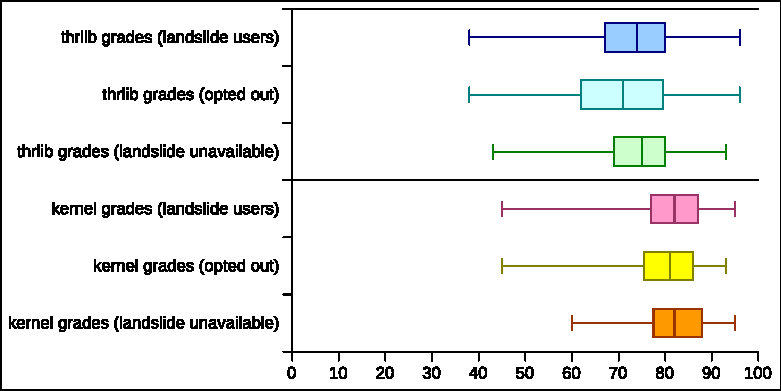
\includegraphics[width=0.96\textwidth]{p2-p3-distribution.pdf}
	\end{center}
	\caption{Distribution of P2 (thrlib) and P3 (kernel) grades among students who did or didn't use Landslide.}
	\label{fig:grade-distribution}
\end{figure}


{\bf Future work.}
One evaluation question remains which I will answer in the thesis:
what is the accuracy of Landslide's automation heuristics (see previous section)?
In other words, were false-positive infinite loops or deadlocks ever reported
where Landslide failed to recognize an ad-hoc synchronization?
(I expect a near 100\% success rate,
having tuned the heuristics by hand on an (independent) set of P2 submissions already.)

\section{Landslide as a Grading Tool}
\label{sec:grading}

TODO

\chapter{Broader Impact}
\label{chap:lipservice}

In this chapter I propose to add several enhancements to Landslide to apply its techniques beyond CMU's walls.
%with little to no manual instrumentation effort required.
This is the third of the three projects I am proposing for this thesis and so far exists only in dreams.
The project will have two parts: adding support for Pintos \cite{pintos}, and adding support for Transactional Memory \cite{transactional-memory}.

\section{Pintos}
\label{sec:pintos-todo}

The Pintos architecture \cite{pintos}, outlined in Section~\ref{sec:overview-pintos}, provides an opportunity to test Landslide's pedagogical mettle beyond CMU's walls.
However, the existing scheduler and concurrency primitives which Pintos provides somewhat limits the remaining concurrency-critical code left to write,
hence limiting the degree to which Landslide can test student submissions.
This is in contrast to the Pebbles assignments at CMU, in which students must implement all the functionality listed in Section~\ref{sec:overview-pintos}.
On the other hand, the upside of Pintos providing substantially more basecode than Pebbles is that most, if not all, of Landslide's kernel instrumentation can be done automatically,
using the names of the core scheduler functions already provided.
For the experiments in Chapter~\ref{chap:quicksand}, I already implemented rudimentary support to test Pintos kernels, but more remains to be done.

{\bf Stuff I already did.}
The existing Pintos support includes
a new set of annotations (e.g., {\tt mutex\_lock} in Pebbles is now called {\tt sema\_down};
handling several quirks of the basecode's scheduling behaviour (ask me if you really care to know);
extending the heap tracker to handle Pintos's page allocator {\tt palloc} as well as the kernel {\tt malloc},
as well as the fact that kernel memory is not direct-mapped like in Pebbles;
new thread-liveness code to detect when a test case terminates;
skipping some busy-wait loops in the boot sequence used for device communication,
a complicated fall-back case in Landslide's timer injection algorithm the workings of which I don't even remember anymore,
and extending the lock-set analysis to include Pintos's interrupt-disabling infrastructure (which was actually pretty tricky when using vector clocks for pure-HB).
All these features apply to behaviours included with the stock base-code, so should apply generally to all but the most adventurous student implementations.

{\bf Stuff I still need to do.}
However, as you might have guessed, there are still a few cases where the existing instrumentation is not fully general.
When preparing Chapter~\ref{chap:quicksand}'s experiments, I needed to adjust some student submissions to be compatible with Landslide's existing annotation process.
In order to distribute Landslide for student use beyond CMU, it will need to support these cases automatically.
These include:
\begin{itemize}
	\item Allowing for the priority scheduler's runqueues to be implemented as an array of queues, rather than the single queue head as provided in the basecode.
	\item Insert the {\tt tell\_landslide\_sleeping} annotation more intelligently than looking for a {\tt list\_insert\_ordered} call (a basecode function which most, but not all, students use).
	\item Some versions of the basecode distribute a {\tt sema\_up} implementation which {\tt yield}s unconditionally, which Landslide must bypass.
	\item Some students use {\tt timer\_sleep} or {\tt while (!flag) continue} when they should use {\tt yield}, which can lead to false-positive deadlocks if not automatically replaced.
	\item I'm sure I've forgotten some less-common ones, which I expect to handle on-the-fly when students email me Landslide crash reports.
\end{itemize}
When fixing my sample of Pintoses by hand, there were also myriad deterministic bugs, such as use-after-frees e.g.~arising from unsafe {\tt strlen} calls.
As with Pebbles student experiments, however, I intend the students to encounter such bug reports and fix them on their own, despite not being concurrency bugs.
It would be a Ph.D. unto itself to automatically ensure stable determinized execution of arbitrary student code.
Actually, probably outright impossible.

{\bf New emulation platform.}
Most importantly, I will need to free Landslide from its dependence on Simics, which requires paid licenses for use beyond CMU's walls.
Other candidate emulation (simulation or virtualization) platforms for Landslide include Bochs, QEMU, VMWare, and Xen.
I am presently studying which of these will most suit Landslide's needs,
but so far Bochs seems like the best bet, which happens to be the simulator used at Berkeley, Stanford, and U. of Chicago anyway.

{\bf Experimental goals.}
Having only one semester (ideally; or two, if my timeline ends up delayed) to test Landslide with Pintos students,
I'll be unable to gather as comprehensive a dataset as I have with 15-410 at CMU.
This will serve more as a proof-of-concept, demonstrating that MC can realistically replace stress testing in operating systems courses worldwide.
Nevertheless, I intend also to analyze what little data I can gather, comparing the incidences and types of bugs found between Pebbles and Pintos populations.
This will perhaps shed light on the advantages and/or shortcomings of either project,
leading to recommendations for improving either project's educational value (independently of using MC).

\section{Transactional Memory}
\label{sec:tm}

Transactional Memory (TM) is a mechanism by which programmers may avoid conventional concurrency primitives, optimizing for performance in the common case when threads do not conflict.
A transactional program surrounds its critical section(s) with transaction begin/end statements, which ensure that no other thread can observe an intermediate state during the transaction.
If a conflict is observed, the transaction {\em aborts}, rolling the program back to the transaction's initial state, and executing an optional back-up code path.
The programmer may also explicitly abort the transaction using an abort statement.
An example transactional program is shown in Figure~\ref{fig:txn-example}.

\begin{figure}[t]
	\begin{center}
	\begin{tabular}{ll}
		\multicolumn{2}{c}{Initially {\tt int foo, bar = 0; mutex\_t m;}} \\
		\\
		\begin{tabular}{l}
		{\bf Thread 1} \\
		\hline
		\texttt{if (\_xbegin() ==} \\
		\texttt{~~~~~~~~\_XBEGIN\_STARTED) \{} \\
		\texttt{~~~~foo++;} \\
		\texttt{~~~~\_xend();} \\
		\texttt{\} else \{} \\
		\texttt{~~~~mutex\_lock(\&m);} \\
		\texttt{~~~~assert(foo > 0 ||} \\
		\texttt{~~~~~~~~~~~bar > 0);} \\
		\texttt{~~~~mutex\_unlock(\&m);} \\
		\texttt{\}} \\
		\end{tabular}
		&
		\begin{tabular}{l}
		{\bf Thread 2} \\
		\hline
		\texttt{if (\_xbegin() ==} \\
		\texttt{~~~~~~~~\_XBEGIN\_STARTED) \{} \\
		\texttt{~~~~bar++;} \\
		\texttt{~~~~\_xend();} \\
		\texttt{\} else \{} \\
		\texttt{~~~~mutex\_lock(\&m);} \\
		\texttt{~~~~assert(foo > 0 ||} \\
		\texttt{~~~~~~~~~~~bar > 0);} \\
		\texttt{~~~~mutex\_unlock(\&m);} \\
		\texttt{\}} \\
		\end{tabular}
	\end{tabular}
	\end{center}
	\caption{Example transactional program, written using GCC's transactional memory compiler intrinsics \cite{htm-gcc}.
	%The x86 assembly instructions are named {\tt xbegin}, {\tt xend}, and {\tt xabort}; I have named the functions of this imaginary C interface the same.
	Different behaviours are possible depending whether the transactions are backed by HTM or STM.}
	\label{fig:txn-example}
\end{figure}

TM may be implemented either in hardware (HTM) \cite{htm-haswell}, or in software (STM) \cite{stm-pldi06}.
Though their interfaces to the programmer are similar, their semantics demand a slightly different treatment from Landslide's perspective.
The key difference is that HTM transactions may fail for any reason, beyond the scope of the program's behaviour, such as the CPU's cache being too full.
STM transactions, on the other hand, will fail only if an actual conflict is observed from another thread.

Consider again the example program: The transactions of the two threads do not conflict, so they may abort only under HTM.
However, when they abort for a reason other than a conflict on {\tt foo} or {\tt bar}, the assertions in the backup code will fail.
Hence, some programs which are correct under STM may contain bugs under HTM.
Supporting TM in Landslide will consist of several steps, extending the concurrency model to incorporate failure injections and extending DPOR to determine when transaction aborts are possible depending on the underlying TM mechanism.

\subsection{HTM}

{\bf Mutex isomorphism.}
When modelling TM in Landslide, we do not care about fidelity to performance characteristics or non-observable roll-back semantics.
The goal of model checking is to exercise all observable program behaviours,
so Landslide can model the execution of transactional programs using existing primitives if possible.
In the first stage of the project, I will prove that a transactional program using is equivalent to one with a global mutex swapped for its {\tt xbegin}s and {\tt xend}s (assuming a retry-only policy for handling aborts).
This will allow Landslide to test all observable TM behaviours using its existing infrastructure for mutexes,
rather than relying on the platform providing accurate TM emulation.

{\bf Abort nondeterminism.}
Next, I will extend the concurrency model to support the nondeterminism arising from transaction aborts.
During execution, Landslide inject a failure to force threads to branch into backup code paths.
Failure injections add an extra ``dimension'' of non-determinism:
at each {\tt xbegin} operation which is a preemption point, Landslide may force a normal context switch to re-interleave threads, or it may inject a transaction abort to test the backup code.
(This also avoids the need to speculatively execute and/or roll-back failing transactions.)
Because HTM transactions can fail for any reason, outside of the programmer's control, Landslide's DPOR implementation will consider failure injections always ``enabled''.

{\bf Reduction challenge.}
I've identified a case under abort nondeterminism in which the current implementation of DPOR will fail to achieve a possible reduction.
Let $1A$, $1B$, $2A$, and $2B$ denote the transitions which execute the {\tt if} and {\tt else} branches by each thread, respectively.
Note that $1A$ conflicts with $2B$, and $1B$ with $2A$, but $1A$ and $2A$ are independent, as are $1B$ and $2B$.
Figure~\ref{fig:txn-graph} provides a visual aid.
There are two possible reductions: pruning $2A,1A$ after testing $1A,2A$, and pruning $2B,1B$ after testing $1B,2B$;
in other words, branches 5 and 8 can be skipped.
However, %if we simply extended DPOR to always inject failures when possible,
our current DPOR implementation will tag the $2B$ subtree to explore after observing the conflict in branch 2 (likewise the $2A$ subtree from branch 3),
but then have no memory of whether it was subsequently supposed to run $1A$ or $1B$, and have to try both.
To fix this will require an optimization analogous to ``sleep sets'' \cite{dpor}:
the tag to explore the $2A$ or $2B$ subtree must include an annotation to remember whether or not the conflict arose after a failure injection in $1$.

\begin{figure}[t]
	\begin{center}
		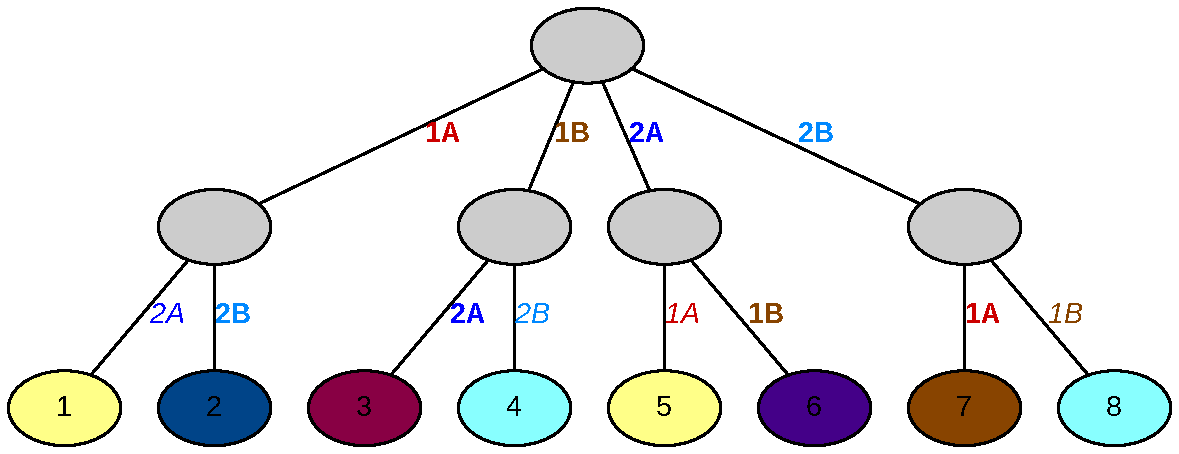
\includegraphics[width=0.8\textwidth]{htm-graph.pdf}
	\end{center}
	\caption{State space corresponding to the program in Figure~\ref{fig:txn-example}.
	Conflicting transitions are marked in bold;
	transitions which are independent from their predecessors are italicized.
	End states colored the same (the cyan and yellow ones) are equivalent.
	}
	\label{fig:txn-graph}
\end{figure}

\subsection{STM}

STM transactions abort only when multiple threads conflict.
Because Landslide already computes memory conflicts among each pair of transitions, it will be natural to extend DPOR to consult the conflict set when deciding whether to exercise a failure injection.
I will extend Landslide in this manner, and even support programs with both types of transactions, as long as the different {\tt xbegin} invocations are suitably annotated.

\subsection{Hybrid HTM/STM}

A recent paper \cite{hybrid-htm-stm} introduced several ways of combining HTM and STM in the same program, nesting transactions of different types.
It presented several semantics for such transactions transactions, the most interesting of which being ``open nesting'', in which a nested transaction's state becomes visible to other threads even during a containing transaction.
That state can then be rolled back if the latter aborts.
I plan to develop a theoretical model for how such transactions would affect Landslide's concurrency model,
although I expect to relegate any implementation thereof to future work.





%Reduction
%techniques such as Dynamic Partial Order Reduction \cite{dpor} and Maximal Causality Reduction \cite{mcr} expand the limits of feasible test completion,
%and search ordering strategies such as Iterative Context Bounding \cite{chess-icb} \revision{encourage}~bugs to be found sooner in a given space should they exist.


%Topics of thesis:
%1. Data race preemption points / iterative deepening
%2. Education in 410. Evaluation questions are:
%	2a. Does P2 submission quality improve?
%	2b. Does P3 submission quality improve correlated with students who used (got the most out of) Landslide during P2?
%	2c. Does Landslide reach the bottom of the class? (Look at bottom-of-class P0s/P1s, see how they improve)
%3. Broader impact
%	3a. Real world programs (and the challenges therein?)
%	3b. Give to pintos kids (and open-source landslide on bochs in doing so)

\chapter{Conclusion and Timeline}

Stateless model checking is a powerful technique for testing concurrent programs,
capable in theory of rooting out any bug or providing total verification on any program,
but suffers several problems which relegate that theory to fantasy land \cite{vargomax}.
Chief among those problems is exponential explosion of state spaces,
making it difficult to decide in advance which combinations of preemption points can be productively tested within a given time limit.
Another major problem is the manual annotation effort required to test certain types of concurrent programs,
which is especially relevant for operating systems students who implement their own kernels.
In this document I have proposed a thesis which will solve both problems.
I leave you now with a proposed timeline for bringing each project to fruition.

\begin{itemize}
	\item TODO % TODO
\end{itemize}

% TODO - make a timeline

%\appendix
%\include{appendix}

\backmatter

%\renewcommand{\baselinestretch}{1.0}\normalsize

% By default \bibsection is \chapter*, but we really want this to show
% up in the table of contents and pdf bookmarks.
\renewcommand{\bibsection}{\chapter{\bibname}}
%\newcommand{\bibpreamble}{This text goes between the ``Bibliography''
%  header and the actual list of references}
\bibliographystyle{plainnat}
\bibliography{citations} %your bib file

\end{document}
